%    Latex Template for ACA 2015
%%%%%%%%%%%%%%%%%%%%%%%%%%%%%%%%%%%%%%%%
%    DO NOT CHANGE THE SETTINGS BELOW
%%%%%%%%%%%%%%%%%%%%%%%%%%%%%%%%%%%%%%%%
\documentclass[11pt]{article}
\usepackage{epsfig}
\usepackage{graphicx}
\usepackage[latin1]{inputenc}
\usepackage[T1]{fontenc}
\usepackage{mathptmx}
\usepackage{url}


\begin{document}



%%%%%%%%%%%%%%%%%%%%%%%%
%%%%%%%%%%%%%%%%%%%%%%%%%%%%%%%%%%%%%%%%
%    DO NOT CHANGE THE SETTINGS ABOVE
%%%%%%%%%%%%%%%%%%%%%%%%%%%%%%%%%%%%%%%%
%
\vspace{-0.8cm}
\begin{flushleft}
\Large \textbf{\noindent
%%% PLEASE INSERT THE TITLE OF YOUR TALK HERE %%%%%%%
Collaborative Use of KeTCindy and Free CASs for Making Materials}
%%%%%%%%%%%%%%%%%%%%%%%%%%%%%%%%%%%%%%%%%%%%%%%%%%%%%%%%
\\
%%%%%%%%%%%%%%%%%%%%%%%%%%%%%%
\vspace{0.5cm}
\normalsize
 %%%%%%             NAMES OF AUTHORS         %%%%%%
 %%%%%% NAME OF SPEAKER SHOULD BE UNDERLINED %%%%%%%%%
\normalsize{
 %%%%%% FOR EXAMPLE %%%%%
 \underline{Setsuo Takato}$^1$, Alasdair McAndrew$^2$,
Masataka Kaneko$^3$
 %%%%%%%%%%%%%%%%%%%%%%%%
} \\
\vspace{5mm}
\textit{\footnotesize
 %%%%%% AFFILIATION OF AUTHORS %%%%%%
$^1$ Toho University, Japan,
takato@phar.toho-u.ac.jp\\
$^2$ Victoria University, Australia,
Alasdair.McAndrew@vu.edu.au\\
$^3$ Toho University, Japan,
masataka.kaneko@phar.toho-u.ac.jp\\
 %%%%%%%%%%%%%%%%%%%%%%%%%%%%%%%%%%%%%
}
\end{flushleft}

\ifnum 1=0

Use this format (without changing the settings) to prepare your abstract. The
abstracts are used for evaluation purposes. Therefore, it is important that you
describe your intended presentation concisely and clearly, including the objectives,
status, methodology, results, and significance of your study.  Abstracts may contain
equations, figures and references (see Eqs.~(\ref{eq1}, \ref{eq2}) and
Refs.~\cite{KR,WK,ABS}). {\bf The extended abstract length is limited to 5 pages}.
Equations are to be centered horizontally, with equation numbers aligned with the
right margin.  Paragraph text is full-justified.  Do not explicitly begin by writing
the word ``abstract''.  Equations should be properly punctuated.  For instance, as
\begin{equation}
y=3x^2\  \  \  \mbox{and}\  \  \  x>0, \label{eq1}
\end{equation}
we see that
\begin{equation}
z=\sqrt{y}=\sqrt{3}x. \label{eq2}
\end{equation}


%\begin{eqnarray}
%\lim_{x \to +\infty} {\rm Abstract}(x) = 1\ {\rm page}.
%\label{eq1}
%\end{eqnarray}
Your abstract should be prepared in \LaTeX\ according to the template provided
and then \textbf{converted to PDF for submission.}  Abstracts not complying with
this template may not be included in the book of abstracts of the ACA
2015. Abstract submission should be done via the session organizers, they will
confirm your submission. If your abstract is accepted, you will be invited to
present your talk.  The book of abstracts will be available to the participants
prior to the conference and will provide the audience with more information
about the papers being presented at the ACA 2015 Workshop. At least one author
must be registered for your talk to be included in the program of the
conference.

\fi

%Copyright (C)  2014  Setsuo Takato, KETpic developer team
%* 
%* This program is free software: you can redistribute it and/or modify
%* it under the terms of the GNU General Public License as published by
%* the Free Software Foundation; either version 3 of the License, or
%* (at your option) any later version.
%* 
%* This program is distributed in the hope that it will be useful,
%* but WITHOUT ANY WARRANTY; without even the implied warranty of
%* MERCHANTABILITY or FITNESS FOR A PARTICULAR PURPOSE.  See the
%* GNU General Public License for more details.
%* 
%* You should have received a copy of the GNU General Public License
%* along with this program.  If not, see <http://www.gnu.org/licenses/>
%%% ketpic.sty
%   2010.09.17 %
%   2016.04.07
%       ketcindy, selarrow, serarrow, nelarrow, nerarrow  
\newcounter{ketpicctra}%
\newcounter{ketpicctrb}%
\newcounter{ketpicctrc}%
\newcounter{ketpicctrd}%
\newcounter{ketpicctre}%
\newcounter{ketpicctrf}%
\newcounter{ketpicctrg}%
\newcounter{ketpicctrh}%
\newcounter{ketpicctri}%
\newcounter{ketpicctrj}%
\def\ketpic{%
{K\kern-.20em\lower.5ex\hbox{E}\kern-.125em{Tpic}}%
%
}%
\def\ketcindy{{K\kern-.20em%
\lower.5ex\hbox{E}\kern-.125em{TCindy}}}%
\def\KeTpic{\ketpic}%
\def\KeTCindy{\ketcindy}%
\newlength{\Width}%
\newlength{\Height}%
\newlength{\Depth}%
\newcommand{\Ltab}[2]{%
\settowidth{\Width}{#2}%
\setlength{\Width}{-\Width}%
\addtolength{\Width}{#1}%
#2\hspace{\Width}\mbox{}%
%
}%
\newcommand{\Rtab}[2]{%
\settowidth{\Width}{#2}%
\setlength{\Width}{-\Width}%
\addtolength{\Width}{#1}%
\hspace*{\Width}#2\mbox{}%
%
}%
\newcommand{\Ctab}[2]{%
\settowidth{\Width}{#2}%
\setlength{\Width}{-\Width}%
\addtolength{\Width}{#1}%
\setlength{\Width}{0.5\Width}%
\hspace*{\Width}#2\hspace{\Width}\mbox{}%
%
}%
\newcommand{\vbackward}[1]{%
\settoheight{\Height}{#1}%
\vspace*{-\Height}%
%
}%
\newcommand{\vforward}[1]{%
\settoheight{\Height}{#1}%
\vspace*{\Height}%
%
}%
\newcommand{\usepack}{%
\usepackage{amsmath,amssymb}%
\usepackage{graphicx}%
\usepackage{color}%
%
}%
\newcommand{\setmargin}[4]{%
\setlength{\oddsidemargin}{-25.4mm}%
\addtolength{\oddsidemargin}{#1 mm}%
\setlength{\textwidth}{\paperwidth}%
\addtolength{\textwidth}{-#1 mm}%
\addtolength{\textwidth}{-#2 mm}%
\setlength{\headheight}{0mm}%
\setlength{\headsep}{0mm}%
\setlength{\topmargin}{-25.4mm}%
\addtolength{\topmargin}{#3 mm}%
\setlength{\textheight}{\paperheight}%
\addtolength{\textheight}{-#3 mm}%
\addtolength{\textheight}{-#4 mm}%
%
}%
\newcommand{\ketcalcwidth}[2][0]{%
\settowidth{\Depth}{#2}%
\setlength{\Width}{0\unitlength}%
\setcounter{ketpicctra}{0}%
\setcounter{ketpicctra}{1}%
\addtocounter{ketpicctra}{-1}%
%
{%
\loop%
\addtocounter{ketpicctra}{1}%
\addtolength{\Width}{\unitlength}%
%
{%
\ifdim %
\Width>\Depth  %
\addtocounter{ketpicctra}{6000}%
%
\fi%
}%
%
\ifnum\theketpicctra<5000%
\repeat%
}%
\addtocounter{ketpicctra}{-6000}%
%
{%
\ifnum %
#1>0 %
\theketpicctra%
%
\fi%
}%
%
}%
\newcommand{\ketcalcheight}[2][0]{%
\settoheight{\Depth}{#2}%
\setlength{\Height}{0\unitlength}%
\setcounter{ketpicctra}{0}%
\setcounter{ketpicctra}{1}%
\addtocounter{ketpicctra}{-1}%
%
{%
\loop%
\addtocounter{ketpicctra}{1}%
\addtolength{\Height}{\unitlength}%
%
{%
\ifdim %
\Height>\Depth  %
\addtocounter{ketpicctra}{6000}%
%
\fi%
}%
%
\ifnum\theketpicctra<5000%
\repeat%
}%
\addtocounter{ketpicctra}{-6000}%
%
{%
\ifnum %
#1>0 %
\theketpicctra%
%
\fi%
}%
%
}%
\newcommand{\ketcalcdepth}[2][0]{%
\settodepth{\Width}{#2}%
\setlength{\Depth}{0\unitlength}%
\setcounter{ketpicctra}{0}%
\setcounter{ketpicctra}{1}%
\addtocounter{ketpicctra}{-1}%
%
{%
\loop%
\addtocounter{ketpicctra}{1}%
\addtolength{\Depth}{\unitlength}%
%
{%
\ifdim %
\Depth>\Width  %
\addtocounter{ketpicctra}{5000}%
%
\fi%
}%
%
\ifnum\theketpicctra<5000%
\repeat%
}%
\addtocounter{ketpicctra}{-5000}%
%
{%
\ifnum %
#1>0 %
\theketpicctra%
%
\fi%
}%
%
}%
\newcommand{\ketcalcwh}[1]{%
{\unitlength=0.1mm%
\ketcalcwidth{#1}%
\setcounter{ketpicctrb}{\value{ketpicctra}}%
\divide\value{ketpicctrb} by 10%
\addtocounter{ketpicctrb}{0}%
\{\theketpicctrb.%
\multiply\value{ketpicctrb} by 10%
\addtocounter{ketpicctrb}{0}%
\addtocounter{ketpicctra}{-\value{ketpicctrb}}%
\theketpicctra\}\{%
\ketcalcheight{#1}%
\setcounter{ketpicctrb}{\value{ketpicctra}}%
\ketcalcdepth{#1}%
\addtocounter{ketpicctra}{\value{ketpicctrb}}%
\setcounter{ketpicctrb}{\value{ketpicctra}}%
\divide\value{ketpicctrb} by 10%
\addtocounter{ketpicctrb}{0}%
\theketpicctrb.%
\multiply\value{ketpicctrb} by 10%
\addtocounter{ketpicctrb}{0}%
\addtocounter{ketpicctra}{-\value{ketpicctrb}}%
\theketpicctra\}%
%
}%
%
}%
\newcommand{\dangerbendmark}[1][1]{%
\def\tmpcontents{%
{\unitlength=0.911mm%
\begin{picture}%
(   3.85072,   4.34364)(   3.18982,   4.86836)%
\special{pn 8}%
%
\special{pa 229 -200}\special{pa 211 -204}\special{pa 195 -208}\special{pa 183 -210}%
\special{pa 173 -212}\special{pa 166 -213}\special{pa 160 -214}\special{pa 155 -215}%
\special{pa 151 -215}\special{pa 149 -215}\special{pa 146 -215}\special{pa 143 -216}%
\special{pa 142 -217}\special{pa 141 -218}\special{pa 142 -220}\special{pa 146 -222}%
\special{pa 152 -226}\special{pa 160 -229}\special{pa 169 -233}\special{pa 180 -237}%
\special{pa 190 -241}\special{pa 201 -245}\special{pa 211 -248}\special{pa 221 -252}%
\special{pa 229 -255}\special{pa 235 -258}\special{pa 240 -260}\special{pa 243 -263}%
\special{pa 246 -266}\special{pa 248 -270}\special{pa 250 -275}\special{pa 251 -280}%
\special{pa 252 -286}\special{pa 253 -292}\special{pa 252 -298}\special{pa 249 -302}%
\special{pa 245 -306}\special{pa 240 -309}\special{pa 235 -312}\special{pa 228 -314}%
\special{pa 221 -316}\special{pa 214 -319}\special{pa 207 -320}\special{pa 198 -322}%
\special{pa 190 -324}\special{pa 181 -326}\special{pa 172 -327}\special{pa 163 -328}%
\special{pa 153 -329}\special{pa 142 -330}\special{pa 142 -330}\special{pa 142 -329}%
\special{pa 142 -329}\special{pa 142 -328}\special{pa 142 -328}\special{pa 142 -327}%
\special{pa 142 -327}\special{pa 142 -326}\special{pa 142 -326}\special{pa 142 -325}%
\special{pa 141 -325}\special{pa 141 -324}\special{pa 141 -324}\special{pa 141 -323}%
\special{pa 141 -323}\special{pa 141 -322}\special{pa 141 -322}\special{pa 141 -321}%
\special{pa 141 -321}\special{pa 141 -320}\special{pa 141 -320}\special{pa 141 -319}%
\special{pa 141 -319}\special{pa 141 -318}\special{pa 141 -318}\special{pa 141 -317}%
\special{pa 140 -317}\special{pa 140 -316}\special{pa 140 -316}\special{pa 140 -315}%
\special{pa 140 -315}\special{pa 140 -314}\special{pa 140 -313}\special{pa 140 -313}%
\special{pa 140 -312}\special{pa 140 -312}\special{pa 140 -311}\special{pa 140 -311}%
\special{pa 140 -310}\special{pa 140 -310}\special{pa 140 -309}\special{pa 140 -309}%
\special{pa 139 -308}\special{pa 139 -308}\special{pa 139 -307}\special{pa 139 -307}%
\special{pa 139 -306}\special{pa 139 -306}\special{pa 139 -305}\special{pa 159 -301}%
\special{pa 175 -297}\special{pa 188 -294}\special{pa 198 -293}\special{pa 206 -292}%
\special{pa 211 -291}\special{pa 215 -291}\special{pa 217 -290}\special{pa 218 -290}%
\special{pa 219 -289}\special{pa 219 -289}\special{pa 219 -287}\special{pa 219 -286}%
\special{pa 219 -285}\special{pa 220 -284}\special{pa 220 -283}\special{pa 220 -283}%
\special{pa 219 -282}\special{pa 215 -280}\special{pa 210 -278}\special{pa 201 -275}%
\special{pa 190 -272}\special{pa 179 -268}\special{pa 167 -264}\special{pa 155 -259}%
\special{pa 145 -255}\special{pa 136 -251}\special{pa 128 -246}\special{pa 122 -242}%
\special{pa 118 -238}\special{pa 116 -234}\special{pa 115 -230}\special{pa 114 -225}%
\special{pa 115 -221}\special{pa 115 -216}\special{pa 116 -211}\special{pa 118 -206}%
\special{pa 121 -202}\special{pa 125 -197}\special{pa 132 -194}\special{pa 140 -190}%
\special{pa 150 -188}\special{pa 160 -185}\special{pa 171 -183}\special{pa 183 -181}%
\special{pa 194 -180}\special{pa 205 -178}\special{pa 215 -176}\special{pa 224 -175}%
\special{pa 224 -175}\special{pa 224 -176}\special{pa 224 -176}\special{pa 224 -176}%
\special{pa 224 -177}\special{pa 224 -177}\special{pa 224 -178}\special{pa 225 -178}%
\special{pa 225 -179}\special{pa 225 -179}\special{pa 225 -180}\special{pa 225 -180}%
\special{pa 225 -181}\special{pa 225 -181}\special{pa 225 -182}\special{pa 225 -182}%
\special{pa 226 -183}\special{pa 226 -183}\special{pa 226 -184}\special{pa 226 -184}%
\special{pa 226 -184}\special{pa 226 -185}\special{pa 226 -185}\special{pa 226 -186}%
\special{pa 226 -186}\special{pa 227 -187}\special{pa 227 -187}\special{pa 227 -188}%
\special{pa 227 -188}\special{pa 227 -189}\special{pa 227 -189}\special{pa 227 -190}%
\special{pa 227 -190}\special{pa 227 -191}\special{pa 227 -191}\special{pa 228 -192}%
\special{pa 228 -192}\special{pa 228 -192}\special{pa 228 -193}\special{pa 228 -193}%
\special{pa 228 -194}\special{pa 228 -194}\special{pa 228 -195}\special{pa 228 -195}%
\special{pa 229 -196}\special{pa 229 -196}\special{pa 229 -197}\special{pa 229 -197}%
\special{pa 229 -198}\special{pa 229 -200}\special{sh 1}\special{ip}%
\special{pn 8}%
\special{pa 229 -200}\special{pa 211 -204}\special{pa 195 -208}\special{pa 183 -210}%
\special{pa 173 -212}\special{pa 166 -213}\special{pa 160 -214}\special{pa 155 -215}%
\special{pa 151 -215}\special{pa 149 -215}\special{pa 146 -215}\special{pa 143 -216}%
\special{pa 142 -217}\special{pa 141 -218}\special{pa 142 -220}\special{pa 146 -222}%
\special{pa 152 -226}\special{pa 160 -229}\special{pa 169 -233}\special{pa 180 -237}%
\special{pa 190 -241}\special{pa 201 -245}\special{pa 211 -248}\special{pa 221 -252}%
\special{pa 229 -255}\special{pa 235 -258}\special{pa 240 -260}\special{pa 243 -263}%
\special{pa 246 -266}\special{pa 248 -270}\special{pa 250 -275}\special{pa 251 -280}%
\special{pa 252 -286}\special{pa 253 -292}\special{pa 252 -298}\special{pa 249 -302}%
\special{pa 245 -306}\special{pa 240 -309}\special{pa 235 -312}\special{pa 228 -314}%
\special{pa 221 -316}\special{pa 214 -319}\special{pa 207 -320}\special{pa 198 -322}%
\special{pa 190 -324}\special{pa 181 -326}\special{pa 172 -327}\special{pa 163 -328}%
\special{pa 153 -329}\special{pa 142 -330}%
\special{fp}%
\special{pa 142 -330}\special{pa 142 -330}\special{pa 142 -329}\special{pa 142 -329}%
\special{pa 142 -328}\special{pa 142 -328}\special{pa 142 -327}\special{pa 142 -327}%
\special{pa 142 -326}\special{pa 142 -326}\special{pa 142 -325}\special{pa 141 -325}%
\special{pa 141 -324}\special{pa 141 -324}\special{pa 141 -323}\special{pa 141 -323}%
\special{pa 141 -322}\special{pa 141 -322}\special{pa 141 -321}\special{pa 141 -321}%
\special{pa 141 -320}\special{pa 141 -320}\special{pa 141 -319}\special{pa 141 -319}%
\special{pa 141 -318}\special{pa 141 -318}\special{pa 141 -317}\special{pa 140 -317}%
\special{pa 140 -316}\special{pa 140 -316}\special{pa 140 -315}\special{pa 140 -315}%
\special{pa 140 -314}\special{pa 140 -313}\special{pa 140 -313}\special{pa 140 -312}%
\special{pa 140 -312}\special{pa 140 -311}\special{pa 140 -311}\special{pa 140 -310}%
\special{pa 140 -310}\special{pa 140 -309}\special{pa 140 -309}\special{pa 139 -308}%
\special{pa 139 -308}\special{pa 139 -307}\special{pa 139 -307}\special{pa 139 -306}%
\special{pa 139 -306}\special{pa 139 -305}%
\special{fp}%
\special{pa 139 -305}\special{pa 159 -301}\special{pa 175 -297}\special{pa 188 -294}%
\special{pa 198 -293}\special{pa 206 -292}\special{pa 211 -291}\special{pa 215 -291}%
\special{pa 217 -290}\special{pa 218 -290}\special{pa 219 -289}\special{pa 219 -289}%
\special{pa 219 -287}\special{pa 219 -286}\special{pa 219 -285}\special{pa 220 -284}%
\special{pa 220 -283}\special{pa 220 -283}\special{pa 219 -282}\special{pa 215 -280}%
\special{pa 210 -278}\special{pa 201 -275}\special{pa 190 -272}\special{pa 179 -268}%
\special{pa 167 -264}\special{pa 155 -259}\special{pa 145 -255}\special{pa 136 -251}%
\special{pa 128 -246}\special{pa 122 -242}\special{pa 118 -238}\special{pa 116 -234}%
\special{pa 115 -230}\special{pa 114 -225}\special{pa 115 -221}\special{pa 115 -216}%
\special{pa 116 -211}\special{pa 118 -206}\special{pa 121 -202}\special{pa 125 -197}%
\special{pa 132 -194}\special{pa 140 -190}\special{pa 150 -188}\special{pa 160 -185}%
\special{pa 171 -183}\special{pa 183 -181}\special{pa 194 -180}\special{pa 205 -178}%
\special{pa 215 -176}\special{pa 224 -175}%
\special{fp}%
\special{pa 224 -175}\special{pa 224 -175}\special{pa 224 -176}\special{pa 224 -176}%
\special{pa 224 -176}\special{pa 224 -177}\special{pa 224 -177}\special{pa 224 -178}%
\special{pa 225 -178}\special{pa 225 -179}\special{pa 225 -179}\special{pa 225 -180}%
\special{pa 225 -180}\special{pa 225 -181}\special{pa 225 -181}\special{pa 225 -182}%
\special{pa 225 -182}\special{pa 226 -183}\special{pa 226 -183}\special{pa 226 -184}%
\special{pa 226 -184}\special{pa 226 -184}\special{pa 226 -185}\special{pa 226 -185}%
\special{pa 226 -186}\special{pa 226 -186}\special{pa 227 -187}\special{pa 227 -187}%
\special{pa 227 -188}\special{pa 227 -188}\special{pa 227 -189}\special{pa 227 -189}%
\special{pa 227 -190}\special{pa 227 -190}\special{pa 227 -191}\special{pa 227 -191}%
\special{pa 228 -192}\special{pa 228 -192}\special{pa 228 -192}\special{pa 228 -193}%
\special{pa 228 -193}\special{pa 228 -194}\special{pa 228 -194}\special{pa 228 -195}%
\special{pa 228 -195}\special{pa 229 -196}\special{pa 229 -196}\special{pa 229 -197}%
\special{pa 229 -197}\special{pa 229 -198}%
\special{fp}%
\special{pn 8}%
\end{picture}}%%
}%
\scalebox{#1}{\tmpcontents}%
%
}%
\newcommand{\cautionmark}[1][1]{%
\scalebox{#1}{%
{\unitlength=1mm%
\begin{picture}%
(   4.60000,   3.98372)(  -2.30000,   0.00000)%
\special{pn 8}%
%
\special{pn 12}%
\special{pa -91 -0}\special{pa 91 -0}\special{pa 0 -157}\special{pa -91 -0}%
\special{fp}%
\special{pn 2}%
\special{pa 12 -22}\special{pa 11 -25}\special{pa 10 -29}\special{pa 7 -31}\special{pa 4 -33}%
\special{pa 0 -33}\special{pa -4 -33}\special{pa -7 -31}\special{pa -10 -29}\special{pa -11 -25}%
\special{pa -12 -22}\special{pa -11 -18}\special{pa -10 -15}\special{pa -7 -12}\special{pa -4 -10}%
\special{pa -0 -10}\special{pa 4 -10}\special{pa 7 -12}\special{pa 10 -15}\special{pa 11 -18}%
\special{pa 12 -22}%
\special{fp}%
\special{pa 0 -47}\special{pa 4 -49}\special{pa 8 -54}\special{pa 11 -60}\special{pa 13 -67}%
\special{pa 14 -75}\special{pa 16 -82}\special{pa 17 -88}\special{pa 18 -94}\special{pa 18 -98}%
\special{pa 16 -102}\special{pa 14 -105}\special{pa 11 -108}\special{pa 7 -110}\special{pa 2 -112}%
\special{pa -3 -112}\special{pa -7 -110}\special{pa -11 -108}\special{pa -14 -105}%
\special{pa -16 -102}\special{pa -17 -98}\special{pa -17 -93}\special{pa -17 -88}%
\special{pa -16 -82}\special{pa -15 -75}\special{pa -13 -67}\special{pa -11 -60}\special{pa -8 -53}%
\special{pa -4 -49}\special{pa 0 -47}%
\special{fp}%
\special{pn 8}%
\special{pa 12 -22}\special{pa 11 -25}\special{pa 10 -29}\special{pa 7 -31}\special{pa 4 -33}%
\special{pa 0 -33}\special{pa -4 -33}\special{pa -7 -31}\special{pa -10 -29}\special{pa -11 -25}%
\special{pa -12 -22}\special{pa -11 -18}\special{pa -10 -15}\special{pa -7 -12}\special{pa -4 -10}%
\special{pa -0 -10}\special{pa 4 -10}\special{pa 7 -12}\special{pa 10 -15}\special{pa 11 -18}%
\special{pa 12 -22}\special{sh 1}\special{ip}%
\special{pa 0 -47}\special{pa 4 -49}\special{pa 8 -54}\special{pa 11 -60}\special{pa 13 -67}%
\special{pa 14 -75}\special{pa 16 -82}\special{pa 17 -88}\special{pa 18 -94}\special{pa 18 -98}%
\special{pa 16 -102}\special{pa 14 -105}\special{pa 11 -108}\special{pa 7 -110}\special{pa 2 -112}%
\special{pa -3 -112}\special{pa -7 -110}\special{pa -11 -108}\special{pa -14 -105}%
\special{pa -16 -102}\special{pa -17 -98}\special{pa -17 -93}\special{pa -17 -88}%
\special{pa -16 -82}\special{pa -15 -75}\special{pa -13 -67}\special{pa -11 -60}\special{pa -8 -53}%
\special{pa -4 -49}\special{pa 0 -47}\special{sh 1}\special{ip}%
\end{picture}}%%
}%
%
}%
\newcommand{\circlemark}[2][8]{%
\scalebox{#2}{%
{\unitlength=1mm%
\begin{picture}%
(   4.00000,   4.00000)(  -2.00000,  -2.00000)%
\special{pn 8}%
%
\special{pn #1}%
\special{pa 79 -0}\special{pa 78 -10}\special{pa 76 -20}\special{pa 73 -29}\special{pa 69 -38}%
\special{pa 64 -46}\special{pa 57 -54}\special{pa 50 -61}\special{pa 42 -66}\special{pa 34 -71}%
\special{pa 24 -75}\special{pa 15 -77}\special{pa 5 -79}\special{pa -5 -79}\special{pa -15 -77}%
\special{pa -24 -75}\special{pa -34 -71}\special{pa -42 -66}\special{pa -50 -61}\special{pa -57 -54}%
\special{pa -64 -46}\special{pa -69 -38}\special{pa -73 -29}\special{pa -76 -20}\special{pa -78 -10}%
\special{pa -79 0}\special{pa -78 10}\special{pa -76 20}\special{pa -73 29}\special{pa -69 38}%
\special{pa -64 46}\special{pa -57 54}\special{pa -50 61}\special{pa -42 66}\special{pa -34 71}%
\special{pa -24 75}\special{pa -15 77}\special{pa -5 79}\special{pa 5 79}\special{pa 15 77}%
\special{pa 24 75}\special{pa 34 71}\special{pa 42 66}\special{pa 50 61}\special{pa 57 54}%
\special{pa 64 46}\special{pa 69 38}\special{pa 73 29}\special{pa 76 20}\special{pa 78 10}%
\special{pa 79 -0}%
\special{fp}%
\end{picture}}%%
}%
%
}%
\newcommand{\circleshade}[3][8]{%
\scalebox{#2}{%
{\unitlength=1mm%
\begin{picture}%
(   4.00000,   4.00000)(  -2.00000,  -2.00000)%
\special{pn 8}%
%
\special{pn #1}%
\special{pa 79 -0}\special{pa 78 -10}\special{pa 76 -20}\special{pa 73 -29}\special{pa 69 -38}%
\special{pa 64 -46}\special{pa 57 -54}\special{pa 50 -61}\special{pa 42 -66}\special{pa 34 -71}%
\special{pa 24 -75}\special{pa 15 -77}\special{pa 5 -79}\special{pa -5 -79}\special{pa -15 -77}%
\special{pa -24 -75}\special{pa -34 -71}\special{pa -42 -66}\special{pa -50 -61}\special{pa -57 -54}%
\special{pa -64 -46}\special{pa -69 -38}\special{pa -73 -29}\special{pa -76 -20}\special{pa -78 -10}%
\special{pa -79 0}\special{pa -78 10}\special{pa -76 20}\special{pa -73 29}\special{pa -69 38}%
\special{pa -64 46}\special{pa -57 54}\special{pa -50 61}\special{pa -42 66}\special{pa -34 71}%
\special{pa -24 75}\special{pa -15 77}\special{pa -5 79}\special{pa 5 79}\special{pa 15 77}%
\special{pa 24 75}\special{pa 34 71}\special{pa 42 66}\special{pa 50 61}\special{pa 57 54}%
\special{pa 64 46}\special{pa 69 38}\special{pa 73 29}\special{pa 76 20}\special{pa 78 10}%
\special{pa 79 -0}\special{sh #3}\special{ip}%
\special{pa 79 -0}\special{pa 78 -10}\special{pa 76 -20}\special{pa 73 -29}\special{pa 69 -38}%
\special{pa 64 -46}\special{pa 57 -54}\special{pa 50 -61}\special{pa 42 -66}\special{pa 34 -71}%
\special{pa 24 -75}\special{pa 15 -77}\special{pa 5 -79}\special{pa -5 -79}\special{pa -15 -77}%
\special{pa -24 -75}\special{pa -34 -71}\special{pa -42 -66}\special{pa -50 -61}\special{pa -57 -54}%
\special{pa -64 -46}\special{pa -69 -38}\special{pa -73 -29}\special{pa -76 -20}\special{pa -78 -10}%
\special{pa -79 0}\special{pa -78 10}\special{pa -76 20}\special{pa -73 29}\special{pa -69 38}%
\special{pa -64 46}\special{pa -57 54}\special{pa -50 61}\special{pa -42 66}\special{pa -34 71}%
\special{pa -24 75}\special{pa -15 77}\special{pa -5 79}\special{pa 5 79}\special{pa 15 77}%
\special{pa 24 75}\special{pa 34 71}\special{pa 42 66}\special{pa 50 61}\special{pa 57 54}%
\special{pa 64 46}\special{pa 69 38}\special{pa 73 29}\special{pa 76 20}\special{pa 78 10}%
\special{pa 79 -0}%
\special{fp}%
\end{picture}}%%
}%
%
}%
%  2016.04.07
\newcommand{\nelarrow}[1][1]{%
\scalebox{#1}{\raisebox{-2.5pt}{%
{\unitlength=1pt%
\begin{picture}%
(  10.00000,  10.00000)(  -5.00000,  -5.00000)%
\special{pn 8}%
%
\special{pa -55 55}\special{pa -40 54}\special{pa -24 51}\special{pa -10 45}\special{pa 4 38}%
\special{pa 17 29}\special{pa 28 18}\special{pa 37 5}\special{pa 45 -9}\special{pa 51 -23}%
\special{pa 54 -39}%
\special{fp}%
\special{pa 61 -16}\special{pa 55 -55}\special{pa 37 -20}\special{pa 49 -18}\special{pa 61 -16}%
\special{sh 1}\special{ip}%
\special{pn 1}%
\special{pa 61 -16}\special{pa 55 -55}\special{pa 37 -20}\special{pa 49 -18}\special{pa 61 -16}%
\special{pa 55 -55}%
\special{fp}%
\special{pn 8}%
\end{picture}}%
}}}%
\newcommand{\nerarrow}[1][1]{%
\scalebox{#1}{\raisebox{-2.5pt}{%
{\unitlength=1pt%
\begin{picture}%
(  10.00000,  10.00000)(  -5.00000,  -5.00000)%
\special{pn 8}%
%
\special{pa 39 -54}\special{pa 23 -51}\special{pa 9 -45}\special{pa -5 -37}\special{pa -18 -28}%
\special{pa -29 -17}\special{pa -38 -4}\special{pa -45 10}\special{pa -51 24}\special{pa -54 40}%
\special{pa -55 55}%
\special{fp}%
\special{pa 20 -37}\special{pa 55 -55}\special{pa 16 -61}\special{pa 18 -49}\special{pa 20 -37}%
\special{sh 1}\special{ip}%
\special{pn 1}%
\special{pa 20 -37}\special{pa 55 -55}\special{pa 16 -61}\special{pa 18 -49}\special{pa 20 -37}%
\special{pa 55 -55}%
\special{fp}%
\special{pn 8}%
\end{picture}}%
}}}%
\newcommand{\selarrow}[1][1]{%
\scalebox{#1}{\raisebox{-2.5pt}{%
{\unitlength=1pt%
\begin{picture}%
(  10.00000,  10.00000)(  -5.00000,  -5.00000)%
\special{pn 8}%
%
\special{pa -55 -55}\special{pa -54 -40}\special{pa -51 -24}\special{pa -45 -10}\special{pa -38 4}%
\special{pa -29 17}\special{pa -18 28}\special{pa -5 37}\special{pa 9 45}\special{pa 23 51}%
\special{pa 39 54}%
\special{fp}%
\special{pa 16 61}\special{pa 55 55}\special{pa 20 37}\special{pa 18 49}\special{pa 16 61}%
\special{sh 1}\special{ip}%
\special{pn 1}%
\special{pa 16 61}\special{pa 55 55}\special{pa 20 37}\special{pa 18 49}\special{pa 16 61}%
\special{pa 55 55}%
\special{fp}%
\special{pn 8}%
\end{picture}}%
}}}%
\newcommand{\serarrow}[1][1]{%
\scalebox{#1}{\raisebox{-2.5pt}{%
{\unitlength=1pt%
\begin{picture}%
(  10.00000,  10.00000)(  -5.00000,  -5.00000)%
\special{pn 8}%
%
\special{pa 54 39}\special{pa 51 23}\special{pa 45 9}\special{pa 37 -5}\special{pa 28 -18}%
\special{pa 17 -29}\special{pa 4 -38}\special{pa -10 -45}\special{pa -24 -51}\special{pa -40 -54}%
\special{pa -55 -55}%
\special{fp}%
\special{pa 37 20}\special{pa 55 55}\special{pa 61 16}\special{pa 49 18}\special{pa 37 20}%
\special{sh 1}\special{ip}%
\special{pn 1}%
\special{pa 37 20}\special{pa 55 55}\special{pa 61 16}\special{pa 49 18}\special{pa 37 20}%
\special{pa 55 55}%
\special{fp}%
\special{pn 8}%
\end{picture}}%
}}}%

%%% ketlayer.sty 2013-10-9 6:3
%%% ketlayer131005.sce 2013-10-6 8:47
%   2013.10.05%
\newlength{\layercurrentunit}%
\newcommand{\shadebox}[7][0]{%
\def\tmpcontents{%
{\unitlength=1mm%
\begin{picture}%
( 100.00000, 100.00000)(   0.00000,   0.00000)%
\special{pn 8}%
%
\special{pa 0 0}\special{pa 3937 0}\special{pa 3937 -3937}\special{pa 0 -3937}\special{pa 0 0}%
\special{sh #6}\special{ip}%
\end{picture}}%%
}%
%
{%
\ifnum %
#4<10 %
%
{%
\ifnum %
#5<10 %
\settowidth{\Width}{{\color{#7}\scalebox{0.0#4}[0.0#5]{\tmpcontents}}}\setlength{\Width}{0\Width}%
\settoheight{\Height}{{\color{#7}\scalebox{0.0#4}[0.0#5]{\tmpcontents}}}\settodepth{\Depth}{{\color{#7}\scalebox{0.0#4}[0.0#5]{\tmpcontents}}}\setlength{\Height}{-\Height}%
\put(#2,-#3){\hspace*{\Width}\raisebox{\Height}{{\color{#7}\scalebox{0.0#4}[0.0#5]{\tmpcontents}}}}%
%
\else%
\settowidth{\Width}{{\color{#7}\scalebox{0.0#4}[0.#5]{\tmpcontents}}}\setlength{\Width}{0\Width}%
\settoheight{\Height}{{\color{#7}\scalebox{0.0#4}[0.#5]{\tmpcontents}}}\settodepth{\Depth}{{\color{#7}\scalebox{0.0#4}[0.#5]{\tmpcontents}}}\setlength{\Height}{-\Height}%
\put(#2,-#3){\hspace*{\Width}\raisebox{\Height}{{\color{#7}\scalebox{0.0#4}[0.#5]{\tmpcontents}}}}%
%
\fi%
}%
%
\else%
%
{%
\ifnum %
#5<10 %
\settowidth{\Width}{{\color{#7}\scalebox{0.#4}[0.0#5]{\tmpcontents}}}\setlength{\Width}{0\Width}%
\settoheight{\Height}{{\color{#7}\scalebox{0.#4}[0.0#5]{\tmpcontents}}}\settodepth{\Depth}{{\color{#7}\scalebox{0.#4}[0.0#5]{\tmpcontents}}}\setlength{\Height}{-\Height}%
\put(#2,-#3){\hspace*{\Width}\raisebox{\Height}{{\color{#7}\scalebox{0.#4}[0.0#5]{\tmpcontents}}}}%
%
\else%
\settowidth{\Width}{{\color{#7}\scalebox{0.#4}[0.#5]{\tmpcontents}}}\setlength{\Width}{0\Width}%
\settoheight{\Height}{{\color{#7}\scalebox{0.#4}[0.#5]{\tmpcontents}}}\settodepth{\Depth}{{\color{#7}\scalebox{0.#4}[0.#5]{\tmpcontents}}}\setlength{\Height}{-\Height}%
\put(#2,-#3){\hspace*{\Width}\raisebox{\Height}{{\color{#7}\scalebox{0.#4}[0.#5]{\tmpcontents}}}}%
%
\fi%
}%
%
\fi%
}%
%
{%
\ifnum %
#1>0 %
\boxframese{#2}{#3}{#4}{#5}{}%
%
\fi%
}%
%
}%
\newcommand{\shadeboxse}[7][0]{%
\shadebox[#1]{#2}{#3}{#4}{#5}{#6}{#7}%
%
}%
\newcommand{\shadeboxc}[7][0]{%
\setcounter{ketpicctrd}{-#4}%
\divide\value{ketpicctrd} by 2%
\addtocounter{ketpicctrd}{#2}%
\setcounter{ketpicctre}{-#4}%
\divide\value{ketpicctre} by 2%
\addtocounter{ketpicctre}{#3}%
\shadebox[#1]{\theketpicctrd}{\theketpicctre}{#4}{#5}{#6}{#7}%
%
}%
\newcommand{\shadeboxe}[7][0]{%
\setcounter{ketpicctrd}{#2}%
\setcounter{ketpicctre}{-#4}%
\divide\value{ketpicctre} by 2%
\addtocounter{ketpicctre}{#3}%
\shadebox[#1]{\theketpicctrd}{\theketpicctre}{#4}{#5}{#6}{#7}%
%
}%
\newcommand{\shadeboxw}[7][0]{%
\setcounter{ketpicctrd}{-#4}%
\addtocounter{ketpicctrd}{#2}%
\setcounter{ketpicctre}{-#4}%
\divide\value{ketpicctre} by 2%
\addtocounter{ketpicctre}{#3}%
\shadebox[#1]{\theketpicctrd}{\theketpicctre}{#4}{#5}{#6}{#7}%
%
}%
\newcommand{\shadeboxn}[7][0]{%
\setcounter{ketpicctrd}{-#4}%
\divide\value{ketpicctrd} by 2%
\addtocounter{ketpicctrd}{#2}%
\setcounter{ketpicctre}{#3}%
\addtocounter{ketpicctre}{-#4}%
\shadebox[#1]{\theketpicctrd}{\theketpicctre}{#4}{#5}{#6}{#7}%
%
}%
\newcommand{\shadeboxs}[7][0]{%
\setcounter{ketpicctrd}{-#4}%
\divide\value{ketpicctrd} by 2%
\addtocounter{ketpicctrd}{#2}%
\setcounter{ketpicctre}{#3}%
\shadebox[#1]{\theketpicctrd}{\theketpicctre}{#4}{#5}{#6}{#7}%
%
}%
\newcommand{\shadeboxnw}[7][0]{%
\setcounter{ketpicctrd}{-#4}%
\addtocounter{ketpicctrd}{#2}%
\setcounter{ketpicctre}{#3}%
\addtocounter{ketpicctre}{-#4}%
\shadebox[#1]{\theketpicctrd}{\theketpicctre}{#4}{#5}{#6}{#7}%
%
}%
\newcommand{\shadeboxne}[7][0]{%
\setcounter{ketpicctrd}{#2}%
\setcounter{ketpicctre}{#3}%
\addtocounter{ketpicctre}{-#4}%
\shadebox[#1]{\theketpicctrd}{\theketpicctre}{#4}{#5}{#6}{#7}%
%
}%
\newcommand{\shadeboxsw}[7][0]{%
\setcounter{ketpicctrd}{-#4}%
\addtocounter{ketpicctrd}{#2}%
\setcounter{ketpicctre}{#3}%
\shadebox[#1]{\theketpicctrd}{\theketpicctre}{#4}{#5}{#6}{#7}%
%
}%
\newcommand{\eraser}[5][0]{%
\def\tmpcontents{%
{\unitlength=1mm%
\begin{picture}%
( 100.00000, 100.00000)(   0.00000,   0.00000)%
\special{pn 8}%
%
\special{pa 0 0}\special{pa 3937 0}\special{pa 3937 -3937}\special{pa 0 -3937}\special{pa 0 0}%
\special{sh 0}\special{ip}%
\end{picture}}%%
}%
%
{%
\ifnum %
#4<10 %
%
{%
\ifnum %
#5<10 %
\settowidth{\Width}{\scalebox{0.0#4}[0.0#5]{\tmpcontents}}\setlength{\Width}{0\Width}%
\settoheight{\Height}{\scalebox{0.0#4}[0.0#5]{\tmpcontents}}\settodepth{\Depth}{\scalebox{0.0#4}[0.0#5]{\tmpcontents}}\setlength{\Height}{-\Height}%
\put(#2,-#3){\hspace*{\Width}\raisebox{\Height}{\scalebox{0.0#4}[0.0#5]{\tmpcontents}}}%
%
\else%
\settowidth{\Width}{\scalebox{0.0#4}[0.#5]{\tmpcontents}}\setlength{\Width}{0\Width}%
\settoheight{\Height}{\scalebox{0.0#4}[0.#5]{\tmpcontents}}\settodepth{\Depth}{\scalebox{0.0#4}[0.#5]{\tmpcontents}}\setlength{\Height}{-\Height}%
\put(#2,-#3){\hspace*{\Width}\raisebox{\Height}{\scalebox{0.0#4}[0.#5]{\tmpcontents}}}%
%
\fi%
}%
%
\else%
%
{%
\ifnum %
#5<10 %
\settowidth{\Width}{\scalebox{0.#4}[0.0#5]{\tmpcontents}}\setlength{\Width}{0\Width}%
\settoheight{\Height}{\scalebox{0.#4}[0.0#5]{\tmpcontents}}\settodepth{\Depth}{\scalebox{0.#4}[0.0#5]{\tmpcontents}}\setlength{\Height}{-\Height}%
\put(#2,-#3){\hspace*{\Width}\raisebox{\Height}{\scalebox{0.#4}[0.0#5]{\tmpcontents}}}%
%
\else%
\settowidth{\Width}{\scalebox{0.#4}[0.#5]{\tmpcontents}}\setlength{\Width}{0\Width}%
\settoheight{\Height}{\scalebox{0.#4}[0.#5]{\tmpcontents}}\settodepth{\Depth}{\scalebox{0.#4}[0.#5]{\tmpcontents}}\setlength{\Height}{-\Height}%
\put(#2,-#3){\hspace*{\Width}\raisebox{\Height}{\scalebox{0.#4}[0.#5]{\tmpcontents}}}%
%
\fi%
}%
%
\fi%
}%
%
{%
\ifnum %
#1>0 %
\boxframese{#2}{#3}{#4}{#5}{}%
%
\fi%
}%
%
}%
\newcommand{\eraserse}[5][0]{%
\eraser[#1]{#2}{#3}{#4}{#5}%
%
}%
\newcommand{\eraserc}[5][0]{%
\setcounter{ketpicctrd}{-#4}%
\divide\value{ketpicctrd} by 2%
\addtocounter{ketpicctrd}{#2}%
\setcounter{ketpicctre}{-#4}%
\divide\value{ketpicctre} by 2%
\addtocounter{ketpicctre}{#3}%
\eraser[#1]{\theketpicctrd}{\theketpicctre}{#4}{#5}%
%
}%
\newcommand{\erasere}[5][0]{%
\setcounter{ketpicctrd}{#2}%
\setcounter{ketpicctre}{-#4}%
\divide\value{ketpicctre} by 2%
\addtocounter{ketpicctre}{#3}%
\eraser[#1]{\theketpicctrd}{\theketpicctre}{#4}{#5}%
%
}%
\newcommand{\eraserw}[5][0]{%
\setcounter{ketpicctrd}{-#4}%
\addtocounter{ketpicctrd}{#2}%
\setcounter{ketpicctre}{-#4}%
\divide\value{ketpicctre} by 2%
\addtocounter{ketpicctre}{#3}%
\eraser[#1]{\theketpicctrd}{\theketpicctre}{#4}{#5}%
%
}%
\newcommand{\erasern}[5][0]{%
\setcounter{ketpicctrd}{-#4}%
\divide\value{ketpicctrd} by 2%
\addtocounter{ketpicctrd}{#2}%
\setcounter{ketpicctre}{#3}%
\addtocounter{ketpicctre}{-#4}%
\eraser[#1]{\theketpicctrd}{\theketpicctre}{#4}{#5}%
%
}%
\newcommand{\erasers}[5][0]{%
\setcounter{ketpicctrd}{-#4}%
\divide\value{ketpicctrd} by 2%
\addtocounter{ketpicctrd}{#2}%
\setcounter{ketpicctre}{#3}%
\eraser[#1]{\theketpicctrd}{\theketpicctre}{#4}{#5}%
%
}%
\newcommand{\erasernw}[5][0]{%
\setcounter{ketpicctrd}{-#4}%
\addtocounter{ketpicctrd}{#2}%
\setcounter{ketpicctre}{#3}%
\addtocounter{ketpicctre}{-#4}%
\eraser[#1]{\theketpicctrd}{\theketpicctre}{#4}{#5}%
%
}%
\newcommand{\eraserne}[5][0]{%
\setcounter{ketpicctrd}{#2}%
\setcounter{ketpicctre}{#3}%
\addtocounter{ketpicctre}{-#4}%
\eraser[#1]{\theketpicctrd}{\theketpicctre}{#4}{#5}%
%
}%
\newcommand{\erasersw}[5][0]{%
\setcounter{ketpicctrd}{-#4}%
\addtocounter{ketpicctrd}{#2}%
\setcounter{ketpicctre}{#3}%
\eraser[#1]{\theketpicctrd}{\theketpicctre}{#4}{#5}%
%
}%
\newcommand{\arrowhead}[4][1]{%
\def\tmpcontents{%
{\unitlength=1mm%
\begin{picture}%
(   4.00000,   1.23607)(  -2.00000,  -0.61803)%
\special{pn 8}%
%
\special{pn 4}%
\special{pa 0 0}\special{pa 79 24}\special{pa 79 -24}\special{pa 0 0}%
\special{fp}%
\special{pn 8}%
\special{pa 0 0}\special{pa 79 24}\special{pa 79 -24}\special{pa 0 0}\special{sh 1}\special{ip}%
\end{picture}}%%
}%
\settowidth{\Width}{\rotatebox[origin=c]{#4}{\scalebox{#1}{\tmpcontents}}}\setlength{\Width}{-0.5\Width}%
\settoheight{\Height}{\rotatebox[origin=c]{#4}{\scalebox{#1}{\tmpcontents}}}\settodepth{\Depth}{\rotatebox[origin=c]{#4}{\scalebox{#1}{\tmpcontents}}}\setlength{\Height}{-0.5\Height}\setlength{\Depth}{0.5\Depth}\addtolength{\Height}{\Depth}%
\put(#2,-#3){\hspace*{\Width}\raisebox{\Height}{\rotatebox[origin=c]{#4}{\scalebox{#1}{\tmpcontents}}}}%
%
}%
\newcommand{\lineseg}[5][12]{%
\def\tmpcontents{%
\setcounter{ketpicctra}{0}%
\setcounter{ketpicctra}{1}%
\addtocounter{ketpicctra}{-1}%
%
{%
\loop%
\addtocounter{ketpicctra}{1}%
{\unitlength=1mm%
\begin{picture}%
(   1.00000,   0.00200)(   0.00000,  -0.00100)%
\special{pn 8}%
%
\special{pn #1}%
\special{pa 0 0}\special{pa 39 0}%
\special{fp}%
\end{picture}}%%
\ifnum\theketpicctra<#4%
\repeat%
}%
%
}%
%
{%
\ifnum %
#5>0 %
%
{%
\ifnum %
#5<90 %
\settowidth{\Width}{\rotatebox[origin=c]{#5}{\tmpcontents}}\setlength{\Width}{0\Width}%
\settoheight{\Height}{\rotatebox[origin=c]{#5}{\tmpcontents}}\settodepth{\Depth}{\rotatebox[origin=c]{#5}{\tmpcontents}}\setlength{\Height}{\Depth}%
\put(#2,-#3){\hspace*{\Width}\raisebox{\Height}{\rotatebox[origin=c]{#5}{\tmpcontents}}}%
%
\else%
\settowidth{\Width}{\rotatebox[origin=c]{#5}{\tmpcontents}}\setlength{\Width}{-1\Width}%
\settoheight{\Height}{\rotatebox[origin=c]{#5}{\tmpcontents}}\settodepth{\Depth}{\rotatebox[origin=c]{#5}{\tmpcontents}}\setlength{\Height}{\Depth}%
\put(#2,-#3){\hspace*{\Width}\raisebox{\Height}{\rotatebox[origin=c]{#5}{\tmpcontents}}}%
%
\fi%
}%
%
\else%
%
{%
\ifnum %
#5>-90 %
\settowidth{\Width}{\rotatebox[origin=c]{#5}{\tmpcontents}}\setlength{\Width}{0\Width}%
\settoheight{\Height}{\rotatebox[origin=c]{#5}{\tmpcontents}}\settodepth{\Depth}{\rotatebox[origin=c]{#5}{\tmpcontents}}\setlength{\Height}{-\Height}%
\put(#2,-#3){\hspace*{\Width}\raisebox{\Height}{\rotatebox[origin=c]{#5}{\tmpcontents}}}%
%
\else%
\settowidth{\Width}{\rotatebox[origin=c]{#5}{\tmpcontents}}\setlength{\Width}{-1\Width}%
\settoheight{\Height}{\rotatebox[origin=c]{#5}{\tmpcontents}}\settodepth{\Depth}{\rotatebox[origin=c]{#5}{\tmpcontents}}\setlength{\Height}{-\Height}%
\put(#2,-#3){\hspace*{\Width}\raisebox{\Height}{\rotatebox[origin=c]{#5}{\tmpcontents}}}%
%
\fi%
}%
%
\fi%
}%
%
}%
\newcommand{\dashlineseg}[5][12]{%
\def\tmpcontents{%
\setcounter{ketpicctra}{0}%
\setcounter{ketpicctra}{1}%
\addtocounter{ketpicctra}{-1}%
%
{%
\loop%
\addtocounter{ketpicctra}{1}%
{\unitlength=1mm%
\begin{picture}%
(   1.00000,   0.00200)(   0.00000,  -0.00100)%
\special{pn 8}%
%
\special{pn #1}%
\special{pa 0 0}\special{pa 20 0}%
\special{fp}%
\end{picture}}%%
\ifnum\theketpicctra<#4%
\repeat%
}%
%
}%
%
{%
\ifnum %
#5>0 %
%
{%
\ifnum %
#5<90 %
\settowidth{\Width}{\rotatebox[origin=c]{#5}{\tmpcontents}}\setlength{\Width}{0\Width}%
\settoheight{\Height}{\rotatebox[origin=c]{#5}{\tmpcontents}}\settodepth{\Depth}{\rotatebox[origin=c]{#5}{\tmpcontents}}\setlength{\Height}{\Depth}%
\put(#2,-#3){\hspace*{\Width}\raisebox{\Height}{\rotatebox[origin=c]{#5}{\tmpcontents}}}%
%
\else%
\settowidth{\Width}{\rotatebox[origin=c]{#5}{\tmpcontents}}\setlength{\Width}{-1\Width}%
\settoheight{\Height}{\rotatebox[origin=c]{#5}{\tmpcontents}}\settodepth{\Depth}{\rotatebox[origin=c]{#5}{\tmpcontents}}\setlength{\Height}{\Depth}%
\put(#2,-#3){\hspace*{\Width}\raisebox{\Height}{\rotatebox[origin=c]{#5}{\tmpcontents}}}%
%
\fi%
}%
%
\else%
%
{%
\ifnum %
#5>-90 %
\settowidth{\Width}{\rotatebox[origin=c]{#5}{\tmpcontents}}\setlength{\Width}{0\Width}%
\settoheight{\Height}{\rotatebox[origin=c]{#5}{\tmpcontents}}\settodepth{\Depth}{\rotatebox[origin=c]{#5}{\tmpcontents}}\setlength{\Height}{-\Height}%
\put(#2,-#3){\hspace*{\Width}\raisebox{\Height}{\rotatebox[origin=c]{#5}{\tmpcontents}}}%
%
\else%
\settowidth{\Width}{\rotatebox[origin=c]{#5}{\tmpcontents}}\setlength{\Width}{-1\Width}%
\settoheight{\Height}{\rotatebox[origin=c]{#5}{\tmpcontents}}\settodepth{\Depth}{\rotatebox[origin=c]{#5}{\tmpcontents}}\setlength{\Height}{-\Height}%
\put(#2,-#3){\hspace*{\Width}\raisebox{\Height}{\rotatebox[origin=c]{#5}{\tmpcontents}}}%
%
\fi%
}%
%
\fi%
}%
%
}%
\def\arrowline#1#2#3#4{%
\lineseg[12]{#1}{#2}{#3}{#4}%
\arrowhead{#1}{#2}{#4}%
%
}%
\newcommand{\arrowlineseg}[5][12]{%
\lineseg[#1]{#2}{#3}{#4}{#5}%
\arrowhead{#2}{#3}{#5}%
%
}%
\newcommand{\conversion}[1]{%
\setcounter{ketpicctra}{#1}%
\multiply\value{ketpicctra} by 3937%
\divide\value{ketpicctra} by 100%
\{\theketpicctra\}%
%
}%
\def\drwline#1#2#3#4{%
\special{pn 8}%
\special{pa #1 #2}\special{pa #3 #4}%
\special{fp}%
%
}%
\newcommand{\dispgrid}[2]{%
\def\tmpcontents{%
{\unitlength=1mm%
\begin{picture}%
(  10.00000,   0.02000)(   0.00000,  -0.01000)%
\special{pn 8}%
%
\special{pn 12}%
\special{pa -6 0}\special{pa 6 0}\special{fp}\special{pa 33 0}\special{pa 45 0}\special{fp}%
\special{pa 73 0}\special{pa 85 0}\special{fp}\special{pa 112 0}\special{pa 124 0}\special{fp}%
\special{pa 151 0}\special{pa 163 0}\special{fp}\special{pa 191 0}\special{pa 203 0}\special{fp}%
\special{pa 230 0}\special{pa 242 0}\special{fp}\special{pa 270 0}\special{pa 282 0}\special{fp}%
\special{pa 309 0}\special{pa 321 0}\special{fp}\special{pa 348 0}\special{pa 360 0}\special{fp}%
\special{pa 388 0}\special{pa 400 0}\special{fp}\special{pn 8}%
\end{picture}}%%
}%
\setcounter{ketpicctre}{#2}%
\divide\value{ketpicctre} by 10%
\setcounter{ketpicctrf}{#1}%
\divide\value{ketpicctrf} by 10%
\addtocounter{ketpicctrf}{-1}%
\setcounter{ketpicctra}{0}%
\setcounter{ketpicctra}{0}%
\addtocounter{ketpicctra}{-1}%
%
{%
\loop%
\addtocounter{ketpicctra}{1}%
\setcounter{ketpicctrd}{0}%
\addtocounter{ketpicctrd}{-\value{ketpicctra}}%
\multiply\value{ketpicctrd} by 10%
\setcounter{ketpicctrc}{0}%
\setcounter{ketpicctrb}{0}%
\setcounter{ketpicctrb}{0}%
\addtocounter{ketpicctrb}{-1}%
%
{%
\loop%
\addtocounter{ketpicctrb}{1}%
\settowidth{\Width}{\tmpcontents}\setlength{\Width}{0\Width}%
\settoheight{\Height}{\tmpcontents}\settodepth{\Depth}{\tmpcontents}\setlength{\Height}{-0.5\Height}\setlength{\Depth}{0.5\Depth}\addtolength{\Height}{\Depth}%
\put(\theketpicctrc,\theketpicctrd){\hspace*{\Width}\raisebox{\Height}{\tmpcontents}}%
\addtocounter{ketpicctrc}{10}%
%
\ifnum\theketpicctrb<\theketpicctrf%
\repeat%
}%
\setcounter{ketpicctrg}{0}%
\addtocounter{ketpicctrg}{-\value{ketpicctrd}}%
\settowidth{\Width}{\theketpicctrg}\setlength{\Width}{-1\Width}%
\settoheight{\Height}{\theketpicctrg}\settodepth{\Depth}{\theketpicctrg}\setlength{\Height}{-0.5\Height}\setlength{\Depth}{0.5\Depth}\addtolength{\Height}{\Depth}%
\put(-1,\theketpicctrd){\hspace*{\Width}\raisebox{\Height}{\theketpicctrg}}%
%
\ifnum\theketpicctra<\theketpicctre%
\repeat%
}%
%
{%
\ifnum %
\theketpicctrd>-#2 %
\setcounter{ketpicctrc}{0}%
\setcounter{ketpicctrb}{0}%
\setcounter{ketpicctrb}{0}%
\addtocounter{ketpicctrb}{-1}%
%
{%
\loop%
\addtocounter{ketpicctrb}{1}%
\settowidth{\Width}{\tmpcontents}\setlength{\Width}{0\Width}%
\settoheight{\Height}{\tmpcontents}\settodepth{\Depth}{\tmpcontents}\setlength{\Height}{-0.5\Height}\setlength{\Depth}{0.5\Depth}\addtolength{\Height}{\Depth}%
\put(\theketpicctrc,-#2){\hspace*{\Width}\raisebox{\Height}{\tmpcontents}}%
\addtocounter{ketpicctrc}{10}%
%
\ifnum\theketpicctrb<\theketpicctrf%
\repeat%
}%
%
\fi%
}%
\def\tmpcontents{%
{\unitlength=1mm%
\begin{picture}%
(   0.02000,  10.00000)(  -0.01000,   0.00000)%
\special{pn 8}%
%
\special{pn 12}%
\special{pa 0 6}\special{pa 0 -6}\special{fp}\special{pa 0 -33}\special{pa 0 -45}\special{fp}%
\special{pa 0 -73}\special{pa 0 -85}\special{fp}\special{pa 0 -112}\special{pa 0 -124}\special{fp}%
\special{pa 0 -151}\special{pa 0 -163}\special{fp}\special{pa 0 -191}\special{pa 0 -203}\special{fp}%
\special{pa 0 -230}\special{pa 0 -242}\special{fp}\special{pa 0 -270}\special{pa 0 -282}\special{fp}%
\special{pa 0 -309}\special{pa 0 -321}\special{fp}\special{pa 0 -348}\special{pa 0 -360}\special{fp}%
\special{pa 0 -388}\special{pa 0 -400}\special{fp}\special{pn 8}%
\end{picture}}%%
}%
\def\tmpcontentsb{%
{\unitlength=1mm%
\begin{picture}%
(   0.02000,   0.02000)(  -0.01000,  -0.01000)%
\special{pn 8}%
%
\special{pa 3 -3}\special{pa -3 -3}\special{pa -3 3}\special{pa 3 3}\special{pa 3 -3}%
\special{sh 1}\special{fp}%
\end{picture}}%%
}%
\setcounter{ketpicctre}{#2}%
\divide\value{ketpicctre} by 10%
\addtocounter{ketpicctre}{-1}%
\setcounter{ketpicctrf}{#1}%
\divide\value{ketpicctrf} by 10%
\setcounter{ketpicctra}{0}%
\setcounter{ketpicctra}{0}%
\addtocounter{ketpicctra}{-1}%
%
{%
\loop%
\addtocounter{ketpicctra}{1}%
\setcounter{ketpicctrd}{0}%
\addtocounter{ketpicctrd}{\value{ketpicctra}}%
\multiply\value{ketpicctrd} by 10%
\setcounter{ketpicctrc}{0}%
\setcounter{ketpicctrb}{0}%
\setcounter{ketpicctrb}{0}%
\addtocounter{ketpicctrb}{-1}%
%
{%
\loop%
\addtocounter{ketpicctrb}{1}%
\settowidth{\Width}{\tmpcontents}\setlength{\Width}{-0.5\Width}%
\settoheight{\Height}{\tmpcontents}\settodepth{\Depth}{\tmpcontents}\setlength{\Height}{-\Height}%
\put(\theketpicctrd,\theketpicctrc){\hspace*{\Width}\raisebox{\Height}{\tmpcontents}}%
\addtocounter{ketpicctrc}{-10}%
%
\ifnum\theketpicctrb<\theketpicctre%
\repeat%
}%
%
{%
\ifnum %
\theketpicctrc>-#2 %
\setcounter{ketpicctrb}{0}%
\setcounter{ketpicctrb}{-#2}%
\addtocounter{ketpicctrb}{-1}%
%
{%
\loop%
\addtocounter{ketpicctrb}{1}%
\settowidth{\Width}{\tmpcontentsb}\setlength{\Width}{-0.5\Width}%
\settoheight{\Height}{\tmpcontentsb}\settodepth{\Depth}{\tmpcontentsb}\setlength{\Height}{-0.5\Height}\setlength{\Depth}{0.5\Depth}\addtolength{\Height}{\Depth}%
\put(\theketpicctrd,\theketpicctrb){\hspace*{\Width}\raisebox{\Height}{\tmpcontentsb}}%
%
\ifnum\theketpicctrb<\theketpicctrc%
\repeat%
}%
%
\fi%
}%
\setcounter{ketpicctrg}{-#2}%
\addtocounter{ketpicctrg}{-1}%
\settowidth{\Width}{\theketpicctrd}\setlength{\Width}{-0.5\Width}%
\settoheight{\Height}{\theketpicctrd}\settodepth{\Depth}{\theketpicctrd}\setlength{\Height}{-\Height}%
\put(\theketpicctrd,\theketpicctrg){\hspace*{\Width}\raisebox{\Height}{\theketpicctrd}}%
%
\ifnum\theketpicctra<\theketpicctrf%
\repeat%
}%
%
}%
\newcommand{\dispgridneg}[2]{%
\def\tmpcontents{%
{\unitlength=1mm%
\begin{picture}%
(  10.00000,   0.02000)(   0.00000,  -0.01000)%
\special{pn 8}%
%
\special{pn 12}%
\special{pa -6 0}\special{pa 6 0}\special{fp}\special{pa 33 0}\special{pa 45 0}\special{fp}%
\special{pa 73 0}\special{pa 85 0}\special{fp}\special{pa 112 0}\special{pa 124 0}\special{fp}%
\special{pa 151 0}\special{pa 163 0}\special{fp}\special{pa 191 0}\special{pa 203 0}\special{fp}%
\special{pa 230 0}\special{pa 242 0}\special{fp}\special{pa 270 0}\special{pa 282 0}\special{fp}%
\special{pa 309 0}\special{pa 321 0}\special{fp}\special{pa 348 0}\special{pa 360 0}\special{fp}%
\special{pa 388 0}\special{pa 400 0}\special{fp}\special{pn 8}%
\end{picture}}%%
}%
\setcounter{ketpicctre}{#2}%
\multiply\value{ketpicctre} by -1%
\divide\value{ketpicctre} by 10%
\setcounter{ketpicctrf}{#1}%
\divide\value{ketpicctrf} by 10%
\addtocounter{ketpicctrf}{-1}%
\setcounter{ketpicctra}{0}%
\setcounter{ketpicctra}{0}%
\addtocounter{ketpicctra}{-1}%
%
{%
\loop%
\addtocounter{ketpicctra}{1}%
\setcounter{ketpicctrd}{\value{ketpicctra}}%
\multiply\value{ketpicctrd} by 10%
\setcounter{ketpicctrc}{0}%
\setcounter{ketpicctrb}{0}%
\setcounter{ketpicctrb}{0}%
\addtocounter{ketpicctrb}{-1}%
%
{%
\loop%
\addtocounter{ketpicctrb}{1}%
\settowidth{\Width}{\tmpcontents}\setlength{\Width}{0\Width}%
\settoheight{\Height}{\tmpcontents}\settodepth{\Depth}{\tmpcontents}\setlength{\Height}{-0.5\Height}\setlength{\Depth}{0.5\Depth}\addtolength{\Height}{\Depth}%
\put(\theketpicctrc,\theketpicctrd){\hspace*{\Width}\raisebox{\Height}{\tmpcontents}}%
\addtocounter{ketpicctrc}{10}%
%
\ifnum\theketpicctrb<\theketpicctrf%
\repeat%
}%
\setcounter{ketpicctrg}{0}%
\addtocounter{ketpicctrg}{-\value{ketpicctrd}}%
\settowidth{\Width}{\theketpicctrg}\setlength{\Width}{-1\Width}%
\settoheight{\Height}{\theketpicctrg}\settodepth{\Depth}{\theketpicctrg}\setlength{\Height}{-0.5\Height}\setlength{\Depth}{0.5\Depth}\addtolength{\Height}{\Depth}%
\put(-1,\theketpicctrd){\hspace*{\Width}\raisebox{\Height}{\theketpicctrg}}%
%
\ifnum\theketpicctra<\theketpicctre%
\repeat%
}%
%
{%
\ifnum %
\theketpicctrd>-#2 %
\setcounter{ketpicctrc}{0}%
\setcounter{ketpicctrb}{0}%
\setcounter{ketpicctrb}{0}%
\addtocounter{ketpicctrb}{-1}%
%
{%
\loop%
\addtocounter{ketpicctrb}{1}%
\settowidth{\Width}{\tmpcontents}\setlength{\Width}{0\Width}%
\settoheight{\Height}{\tmpcontents}\settodepth{\Depth}{\tmpcontents}\setlength{\Height}{-0.5\Height}\setlength{\Depth}{0.5\Depth}\addtolength{\Height}{\Depth}%
\put(\theketpicctrc,-#2){\hspace*{\Width}\raisebox{\Height}{\tmpcontents}}%
\addtocounter{ketpicctrc}{10}%
%
\ifnum\theketpicctrb<\theketpicctrf%
\repeat%
}%
%
\fi%
}%
\def\tmpcontents{%
{\unitlength=1mm%
\begin{picture}%
(   0.02000,  10.00000)(  -0.01000,   0.00000)%
\special{pn 8}%
%
\special{pn 12}%
\special{pa 0 6}\special{pa 0 -6}\special{fp}\special{pa 0 -33}\special{pa 0 -45}\special{fp}%
\special{pa 0 -73}\special{pa 0 -85}\special{fp}\special{pa 0 -112}\special{pa 0 -124}\special{fp}%
\special{pa 0 -151}\special{pa 0 -163}\special{fp}\special{pa 0 -191}\special{pa 0 -203}\special{fp}%
\special{pa 0 -230}\special{pa 0 -242}\special{fp}\special{pa 0 -270}\special{pa 0 -282}\special{fp}%
\special{pa 0 -309}\special{pa 0 -321}\special{fp}\special{pa 0 -348}\special{pa 0 -360}\special{fp}%
\special{pa 0 -388}\special{pa 0 -400}\special{fp}\special{pn 8}%
\end{picture}}%%
}%
\def\tmpcontentsb{%
{\unitlength=1mm%
\begin{picture}%
(   0.02000,   0.02000)(  -0.01000,  -0.01000)%
\special{pn 8}%
%
\special{pa 3 -3}\special{pa -3 -3}\special{pa -3 3}\special{pa 3 3}\special{pa 3 -3}%
\special{sh 1}\special{fp}%
\end{picture}}%%
}%
\setcounter{ketpicctre}{#2}%
\multiply\value{ketpicctre} by -1%
\divide\value{ketpicctre} by 10%
\addtocounter{ketpicctre}{-1}%
\setcounter{ketpicctrf}{#1}%
\divide\value{ketpicctrf} by 10%
\setcounter{ketpicctra}{0}%
\setcounter{ketpicctra}{0}%
\addtocounter{ketpicctra}{-1}%
%
{%
\loop%
\addtocounter{ketpicctra}{1}%
\setcounter{ketpicctrd}{0}%
\addtocounter{ketpicctrd}{\value{ketpicctra}}%
\multiply\value{ketpicctrd} by 10%
\setcounter{ketpicctrc}{0}%
\setcounter{ketpicctrb}{0}%
\setcounter{ketpicctrb}{0}%
\addtocounter{ketpicctrb}{-1}%
%
{%
\loop%
\addtocounter{ketpicctrb}{1}%
\settowidth{\Width}{\tmpcontents}\setlength{\Width}{-0.5\Width}%
\settoheight{\Height}{\tmpcontents}\settodepth{\Depth}{\tmpcontents}\setlength{\Height}{\Depth}%
\put(\theketpicctrd,\theketpicctrc){\hspace*{\Width}\raisebox{\Height}{\tmpcontents}}%
\addtocounter{ketpicctrc}{10}%
%
\ifnum\theketpicctrb<\theketpicctre%
\repeat%
}%
%
{%
\ifnum %
\theketpicctrc>-#2 %
\setcounter{ketpicctrb}{0}%
\setcounter{ketpicctrb}{-#2}%
\addtocounter{ketpicctrb}{-1}%
%
{%
\loop%
\addtocounter{ketpicctrb}{1}%
\settowidth{\Width}{\tmpcontentsb}\setlength{\Width}{-0.5\Width}%
\settoheight{\Height}{\tmpcontentsb}\settodepth{\Depth}{\tmpcontentsb}\setlength{\Height}{-0.5\Height}\setlength{\Depth}{0.5\Depth}\addtolength{\Height}{\Depth}%
\put(\theketpicctrd,\theketpicctrb){\hspace*{\Width}\raisebox{\Height}{\tmpcontentsb}}%
%
\ifnum\theketpicctrb<\theketpicctrc%
\repeat%
}%
%
\fi%
}%
\setcounter{ketpicctrg}{-#2}%
\addtocounter{ketpicctrg}{1}%
\settowidth{\Width}{\theketpicctrd}\setlength{\Width}{-0.5\Width}%
\settoheight{\Height}{\theketpicctrd}\settodepth{\Depth}{\theketpicctrd}\setlength{\Height}{\Depth}%
\put(\theketpicctrd,\theketpicctrg){\hspace*{\Width}\raisebox{\Height}{\theketpicctrd}}%
%
\ifnum\theketpicctra<\theketpicctrf%
\repeat%
}%
%
}%
\newenvironment{layer}[3][0]{%
\setlength{\layercurrentunit}{\unitlength}%
\unitlength=1 mm%
\vspace{-\baselineskip}%
\noindent%
\hspace*{#1 mm}%
\begin{picture}(#3,0)(0,0)%
%
{%
\ifnum %
#3>0 %
\dispgrid{#2}{#3}%
%
\fi%
}%
%
{%
\ifnum %
#3<0 %
\dispgridneg{#2}{#3}%
%
\fi%
}%
}{%
\end{picture}%
\setlength{\unitlength}{\layercurrentunit}%
%
}%
\newenvironment{layerv}[3][0]{%
\setlength{\layercurrentunit}{\unitlength}%
\unitlength=1 mm%
\vspace*{-\baselineskip}%
\vspace*{#2 mm}%

\setcounter{ketpicctrj}{-#2}%
\noindent%
\hspace*{#1 mm}%
\begin{picture}(100,0)(0,0)%
%
{%
\ifnum %
#3>0 %
\setlength{\Width}{\textwidth}%
\addtolength{\Width}{-#1 mm}%
\setcounter{ketpicctri}{0}%
\setcounter{ketpicctri}{1}%
\addtocounter{ketpicctri}{-1}%
%
{%
\loop%
\addtocounter{ketpicctri}{1}%
%
{%
\ifdim %
\theketpicctri mm>\Width %
\addtocounter{ketpicctri}{500}%
%
\fi%
}%
%
\ifnum\theketpicctri<400%
\repeat%
}%
\addtocounter{ketpicctri}{-500}%
\addtocounter{ketpicctri}{-1}%
\dispgrid{\theketpicctri}{#3}%
%
\fi%
}%
}{%
\end{picture}%
\vspace*{\theketpicctrj mm}%
\setlength{\unitlength}{\layercurrentunit}%
%
}%
\newenvironment{layerg}[2][1]{%
\setlength{\layercurrentunit}{\unitlength}%
\unitlength=1 mm%
\vspace*{-\baselineskip}%
\ketcalcheight{#2}%
\setcounter{ketpicctrj}{\value{ketpicctra}}%
\ketcalcdepth{#2}%
\addtocounter{ketpicctrj}{\value{ketpicctra}}%
\vspace*{-\theketpicctrj mm}%

\noindent%
\begin{picture}(100,0)(0,0)%
%
{%
\ifnum %
#1>0 %
\setlength{\Width}{\textwidth}%
\addtolength{\Width}{-#1 mm}%
\setcounter{ketpicctri}{0}%
\setcounter{ketpicctri}{1}%
\addtocounter{ketpicctri}{-1}%
%
{%
\loop%
\addtocounter{ketpicctri}{1}%
%
{%
\ifdim %
\theketpicctri mm>\Width %
\addtocounter{ketpicctri}{500}%
%
\fi%
}%
%
\ifnum\theketpicctri<400%
\repeat%
}%
\addtocounter{ketpicctri}{-500}%
\addtocounter{ketpicctri}{-1}%
\dispgrid{\theketpicctri}{\theketpicctrj}%
%
\fi%
}%
}{%
\end{picture}%
\vspace*{\theketpicctrj mm}%
\setlength{\unitlength}{\layercurrentunit}%
%
}%
\newcommand{\putnotec}[3]{%
\settowidth{\Width}{#3}\setlength{\Width}{-0.5\Width}%
\settoheight{\Height}{#3}\settodepth{\Depth}{#3}\setlength{\Height}{-0.5\Height}\setlength{\Depth}{0.5\Depth}\addtolength{\Height}{\Depth}%
\put(#1,-#2){\hspace*{\Width}\raisebox{\Height}{#3}}%
%
}%
\newcommand{\putnotee}[3]{%
\settowidth{\Width}{#3}\setlength{\Width}{0\Width}%
\settoheight{\Height}{#3}\settodepth{\Depth}{#3}\setlength{\Height}{-0.5\Height}\setlength{\Depth}{0.5\Depth}\addtolength{\Height}{\Depth}%
\put(#1,-#2){\hspace*{\Width}\raisebox{\Height}{#3}}%
%
}%
\newcommand{\putnotew}[3]{%
\settowidth{\Width}{#3}\setlength{\Width}{-1\Width}%
\settoheight{\Height}{#3}\settodepth{\Depth}{#3}\setlength{\Height}{-0.5\Height}\setlength{\Depth}{0.5\Depth}\addtolength{\Height}{\Depth}%
\put(#1,-#2){\hspace*{\Width}\raisebox{\Height}{#3}}%
%
}%
\newcommand{\putnotes}[3]{%
\settowidth{\Width}{#3}\setlength{\Width}{-0.5\Width}%
\settoheight{\Height}{#3}\settodepth{\Depth}{#3}\setlength{\Height}{-\Height}%
\put(#1,-#2){\hspace*{\Width}\raisebox{\Height}{#3}}%
%
}%
\newcommand{\putnoten}[3]{%
\settowidth{\Width}{#3}\setlength{\Width}{-0.5\Width}%
\settoheight{\Height}{#3}\settodepth{\Depth}{#3}\setlength{\Height}{\Depth}%
\put(#1,-#2){\hspace*{\Width}\raisebox{\Height}{#3}}%
%
}%
\newcommand{\putnotene}[3]{%
\settowidth{\Width}{#3}\setlength{\Width}{0\Width}%
\settoheight{\Height}{#3}\settodepth{\Depth}{#3}\setlength{\Height}{\Depth}%
\put(#1,-#2){\hspace*{\Width}\raisebox{\Height}{#3}}%
%
}%
\newcommand{\putnotenw}[3]{%
\settowidth{\Width}{#3}\setlength{\Width}{-1\Width}%
\settoheight{\Height}{#3}\settodepth{\Depth}{#3}\setlength{\Height}{\Depth}%
\put(#1,-#2){\hspace*{\Width}\raisebox{\Height}{#3}}%
%
}%
\newcommand{\putnotese}[3]{%
\settowidth{\Width}{#3}\setlength{\Width}{0\Width}%
\settoheight{\Height}{#3}\settodepth{\Depth}{#3}\setlength{\Height}{-\Height}%
\put(#1,-#2){\hspace*{\Width}\raisebox{\Height}{#3}}%
%
}%
\newcommand{\putnotesw}[3]{%
\settowidth{\Width}{#3}\setlength{\Width}{-1\Width}%
\settoheight{\Height}{#3}\settodepth{\Depth}{#3}\setlength{\Height}{-\Height}%
\put(#1,-#2){\hspace*{\Width}\raisebox{\Height}{#3}}%
%
}%
\newcommand{\ballonr}[5][8]{%
\def\tempcontents{%
{\unitlength=1cm%
\begin{picture}%
(   4.00000,   3.50000)(  -2.00000,   0.00000)%
\special{pn 8}%
%
\special{pn #1}%
\special{pa 124 -260}\special{pa 123 -261}\special{pa 120 -262}\special{pa 115 -263}%
\special{pa 109 -264}\special{pa 101 -266}\special{pa 92 -267}\special{pa 82 -269}%
\special{pa 71 -271}\special{pa 59 -273}\special{pa 45 -276}\special{pa 32 -279}\special{pa 17 -282}%
\special{pa 2 -286}\special{pa -14 -290}\special{pa -30 -295}\special{pa -47 -300}%
\special{pa -63 -306}\special{pa -80 -312}\special{pa -96 -319}\special{pa -112 -327}%
\special{pa -128 -335}\special{pa -144 -344}\special{pa -159 -354}\special{pa -174 -365}%
\special{pa -188 -376}\special{pa -201 -388}\special{pa -213 -401}\special{pa -224 -416}%
\special{pa -234 -431}\special{pa -243 -447}\special{pa -250 -464}\special{pa -256 -482}%
\special{pa -260 -501}\special{pa -263 -522}\special{pa -264 -544}\special{pa -263 -566}%
\special{pa -260 -591}\special{pa -265 -595}\special{pa -274 -599}\special{pa -287 -603}%
\special{pa -302 -607}\special{pa -320 -611}\special{pa -340 -615}\special{pa -360 -620}%
\special{pa -381 -626}\special{pa -402 -633}\special{pa -423 -641}\special{pa -442 -651}%
\special{pa -459 -662}\special{pa -473 -675}\special{pa -484 -691}\special{pa -492 -709}%
\special{pa -496 -728}\special{pa -498 -750}\special{pa -498 -772}\special{pa -496 -794}%
\special{pa -493 -817}\special{pa -490 -839}\special{pa -487 -860}\special{pa -483 -880}%
\special{pa -479 -899}\special{pa -472 -918}\special{pa -464 -935}\special{pa -452 -952}%
\special{pa -437 -969}\special{pa -418 -984}\special{pa -395 -999}\special{pa -370 -1013}%
\special{pa -342 -1026}\special{pa -312 -1037}\special{pa -280 -1048}\special{pa -248 -1057}%
\special{pa -216 -1065}\special{pa -184 -1071}\special{pa -152 -1076}\special{pa -122 -1078}%
\special{pa -95 -1079}\special{pa -69 -1078}\special{pa -47 -1075}\special{pa -37 -1085}%
\special{pa -26 -1095}\special{pa -15 -1106}\special{pa -1 -1117}\special{pa 13 -1129}%
\special{pa 29 -1140}\special{pa 47 -1152}\special{pa 67 -1162}\special{pa 90 -1172}%
\special{pa 114 -1181}\special{pa 142 -1189}\special{pa 172 -1196}\special{pa 205 -1201}%
\special{pa 242 -1205}\special{pa 282 -1206}\special{pa 324 -1206}\special{pa 368 -1204}%
\special{pa 411 -1200}\special{pa 454 -1195}\special{pa 494 -1189}\special{pa 531 -1181}%
\special{pa 565 -1172}\special{pa 594 -1162}\special{pa 619 -1150}\special{pa 642 -1136}%
\special{pa 662 -1120}\special{pa 680 -1102}\special{pa 697 -1081}\special{pa 712 -1057}%
\special{pa 726 -1031}\special{pa 738 -1004}\special{pa 748 -975}\special{pa 755 -945}%
\special{pa 760 -916}\special{pa 762 -886}\special{pa 760 -857}\special{pa 755 -829}%
\special{pa 745 -803}\special{pa 732 -779}\special{pa 713 -758}\special{pa 690 -740}%
\special{pa 661 -726}\special{pa 668 -717}\special{pa 675 -706}\special{pa 681 -695}%
\special{pa 688 -683}\special{pa 694 -670}\special{pa 699 -657}\special{pa 704 -643}%
\special{pa 708 -629}\special{pa 712 -614}\special{pa 715 -599}\special{pa 718 -583}%
\special{pa 719 -567}\special{pa 720 -551}\special{pa 719 -534}\special{pa 718 -518}%
\special{pa 715 -501}\special{pa 712 -484}\special{pa 707 -468}\special{pa 701 -451}%
\special{pa 693 -435}\special{pa 684 -418}\special{pa 673 -402}\special{pa 661 -387}%
\special{pa 648 -372}\special{pa 633 -357}\special{pa 617 -343}\special{pa 600 -329}%
\special{pa 581 -316}\special{pa 560 -304}\special{pa 539 -293}\special{pa 516 -283}%
\special{pa 491 -273}\special{pa 466 -265}\special{pa 439 -258}\special{pa 410 -252}%
\special{pa 381 -247}\special{pa 349 -244}\special{pa 317 -242}\special{pa 283 -242}%
\special{pa 278 -228}\special{pa 273 -215}\special{pa 267 -202}\special{pa 261 -190}%
\special{pa 255 -178}\special{pa 248 -166}\special{pa 242 -155}\special{pa 235 -144}%
\special{pa 228 -133}\special{pa 220 -123}\special{pa 213 -114}\special{pa 205 -104}%
\special{pa 197 -95}\special{pa 189 -87}\special{pa 180 -79}\special{pa 171 -71}\special{pa 162 -63}%
\special{pa 153 -57}\special{pa 144 -50}\special{pa 134 -44}\special{pa 124 -38}\special{pa 114 -33}%
\special{pa 104 -28}\special{pa 93 -23}\special{pa 82 -19}\special{pa 71 -15}\special{pa 60 -11}%
\special{pa 48 -8}\special{pa 37 -6}\special{pa 25 -3}\special{pa 12 -1}\special{pa 0 0}%
\special{pa 8 -6}\special{pa 15 -12}\special{pa 23 -18}\special{pa 30 -25}\special{pa 37 -31}%
\special{pa 43 -38}\special{pa 49 -45}\special{pa 55 -52}\special{pa 61 -59}\special{pa 67 -66}%
\special{pa 72 -73}\special{pa 77 -81}\special{pa 82 -88}\special{pa 86 -96}\special{pa 90 -104}%
\special{pa 94 -112}\special{pa 98 -120}\special{pa 102 -129}\special{pa 105 -137}%
\special{pa 108 -146}\special{pa 111 -155}\special{pa 113 -163}\special{pa 115 -172}%
\special{pa 117 -182}\special{pa 119 -191}\special{pa 121 -200}\special{pa 122 -210}%
\special{pa 123 -220}\special{pa 123 -229}\special{pa 124 -239}\special{pa 124 -250}%
\special{pa 124 -260}%
\special{fp}%
\settowidth{\Width}{{\begin{minipage}{1.8cm}#5\end{minipage}}}\setlength{\Width}{-0.5\Width}%
\settoheight{\Height}{{\begin{minipage}{1.8cm}#5\end{minipage}}}\settodepth{\Depth}{{\begin{minipage}{1.8cm}#5\end{minipage}}}\setlength{\Height}{-0.5\Height}\setlength{\Depth}{0.5\Depth}\addtolength{\Height}{\Depth}%
\put(0.5000,1.8000){\hspace*{\Width}\raisebox{\Height}{{\begin{minipage}{1.8cm}#5\end{minipage}}}}%
%
%
\end{picture}}%%
}%
\setcounter{ketpicctra}{-#3}%
\settowidth{\Width}{{\scalebox{#4}{\tempcontents}}}\setlength{\Width}{-0.5\Width}%
\settoheight{\Height}{{\scalebox{#4}{\tempcontents}}}\settodepth{\Depth}{{\scalebox{#4}{\tempcontents}}}\setlength{\Height}{\Depth}%
\put(#2,\theketpicctra){\hspace*{\Width}\raisebox{\Height}{{\scalebox{#4}{\tempcontents}}}}%
%
}%
\newcommand{\ballonl}[5][8]{%
\def\tempcontents{%
{\unitlength=1cm%
\begin{picture}%
(   5.00000,   2.50000)(  -2.50000,   0.00000)%
\special{pn 8}%
%
\special{pn #1}%
\special{pa -225 -221}\special{pa -262 -199}\special{pa -296 -180}\special{pa -329 -163}%
\special{pa -360 -149}\special{pa -390 -138}\special{pa -419 -128}\special{pa -446 -121}%
\special{pa -473 -116}\special{pa -499 -112}\special{pa -525 -110}\special{pa -550 -109}%
\special{pa -576 -109}\special{pa -602 -111}\special{pa -628 -113}\special{pa -655 -115}%
\special{pa -682 -119}\special{pa -709 -124}\special{pa -736 -131}\special{pa -762 -139}%
\special{pa -786 -151}\special{pa -810 -165}\special{pa -831 -182}\special{pa -851 -202}%
\special{pa -868 -224}\special{pa -883 -248}\special{pa -895 -274}\special{pa -904 -301}%
\special{pa -909 -329}\special{pa -912 -357}\special{pa -910 -386}\special{pa -906 -414}%
\special{pa -898 -441}\special{pa -887 -467}\special{pa -874 -492}\special{pa -857 -515}%
\special{pa -838 -537}\special{pa -817 -555}\special{pa -793 -572}\special{pa -767 -585}%
\special{pa -738 -594}\special{pa -708 -600}\special{pa -676 -602}\special{pa -684 -633}%
\special{pa -688 -663}\special{pa -689 -691}\special{pa -687 -718}\special{pa -681 -743}%
\special{pa -673 -766}\special{pa -663 -788}\special{pa -650 -808}\special{pa -635 -827}%
\special{pa -619 -843}\special{pa -601 -858}\special{pa -582 -871}\special{pa -562 -883}%
\special{pa -541 -892}\special{pa -520 -900}\special{pa -498 -906}\special{pa -476 -911}%
\special{pa -452 -915}\special{pa -427 -918}\special{pa -401 -920}\special{pa -372 -922}%
\special{pa -342 -924}\special{pa -311 -926}\special{pa -279 -927}\special{pa -248 -928}%
\special{pa -217 -927}\special{pa -187 -925}\special{pa -160 -922}\special{pa -136 -918}%
\special{pa -114 -912}\special{pa -94 -904}\special{pa -77 -894}\special{pa -61 -882}%
\special{pa -47 -869}\special{pa -35 -853}\special{pa -23 -836}\special{pa -13 -816}%
\special{pa -3 -794}\special{pa 7 -770}\special{pa 16 -744}\special{pa 25 -715}\special{pa 35 -684}%
\special{pa 56 -683}\special{pa 76 -680}\special{pa 95 -677}\special{pa 112 -672}%
\special{pa 128 -667}\special{pa 142 -661}\special{pa 156 -654}\special{pa 169 -646}%
\special{pa 180 -637}\special{pa 191 -627}\special{pa 202 -616}\special{pa 211 -603}%
\special{pa 221 -590}\special{pa 230 -576}\special{pa 238 -561}\special{pa 246 -545}%
\special{pa 253 -528}\special{pa 258 -510}\special{pa 262 -492}\special{pa 264 -473}%
\special{pa 264 -455}\special{pa 261 -436}\special{pa 257 -417}\special{pa 250 -399}%
\special{pa 242 -382}\special{pa 232 -365}\special{pa 222 -348}\special{pa 212 -333}%
\special{pa 202 -320}\special{pa 192 -307}\special{pa 181 -296}\special{pa 170 -285}%
\special{pa 158 -276}\special{pa 144 -268}\special{pa 130 -260}\special{pa 114 -253}%
\special{pa 96 -246}\special{pa 77 -241}\special{pa 55 -235}\special{pa 31 -230}\special{pa 4 -225}%
\special{pa -26 -221}\special{pa -26 -214}\special{pa -26 -208}\special{pa -26 -201}%
\special{pa -27 -194}\special{pa -26 -187}\special{pa -26 -181}\special{pa -26 -174}%
\special{pa -26 -167}\special{pa -26 -160}\special{pa -25 -154}\special{pa -25 -147}%
\special{pa -24 -140}\special{pa -24 -133}\special{pa -23 -126}\special{pa -22 -119}%
\special{pa -22 -113}\special{pa -21 -106}\special{pa -20 -99}\special{pa -19 -92}%
\special{pa -18 -85}\special{pa -17 -78}\special{pa -16 -71}\special{pa -14 -64}\special{pa -13 -57}%
\special{pa -12 -50}\special{pa -10 -43}\special{pa -9 -36}\special{pa -7 -29}\special{pa -5 -21}%
\special{pa -4 -14}\special{pa -2 -7}\special{pa 0 0}\special{pa -9 -11}\special{pa -17 -21}%
\special{pa -26 -32}\special{pa -34 -42}\special{pa -42 -52}\special{pa -50 -61}\special{pa -58 -71}%
\special{pa -66 -80}\special{pa -74 -88}\special{pa -82 -97}\special{pa -89 -105}%
\special{pa -97 -113}\special{pa -104 -121}\special{pa -111 -129}\special{pa -119 -136}%
\special{pa -126 -143}\special{pa -133 -150}\special{pa -139 -156}\special{pa -146 -162}%
\special{pa -153 -168}\special{pa -160 -174}\special{pa -166 -180}\special{pa -172 -185}%
\special{pa -179 -190}\special{pa -185 -195}\special{pa -191 -199}\special{pa -197 -203}%
\special{pa -203 -207}\special{pa -208 -211}\special{pa -214 -215}\special{pa -220 -218}%
\special{pa -225 -221}%
\special{fp}%
\settowidth{\Width}{{\begin{minipage}{1.5cm}#5\end{minipage}}}\setlength{\Width}{-0.5\Width}%
\settoheight{\Height}{{\begin{minipage}{1.5cm}#5\end{minipage}}}\settodepth{\Depth}{{\begin{minipage}{1.5cm}#5\end{minipage}}}\setlength{\Height}{-0.5\Height}\setlength{\Depth}{0.5\Depth}\addtolength{\Height}{\Depth}%
\put(-0.8000,1.2000){\hspace*{\Width}\raisebox{\Height}{{\begin{minipage}{1.5cm}#5\end{minipage}}}}%
%
%
\end{picture}}%%
}%
\setcounter{ketpicctra}{-#3}%
\settowidth{\Width}{{\scalebox{#4}{\tempcontents}}}\setlength{\Width}{-0.5\Width}%
\settoheight{\Height}{{\scalebox{#4}{\tempcontents}}}\settodepth{\Depth}{{\scalebox{#4}{\tempcontents}}}\setlength{\Height}{\Depth}%
\put(#2,\theketpicctra){\hspace*{\Width}\raisebox{\Height}{{\scalebox{#4}{\tempcontents}}}}%
%
}%
\newcommand{\lefthand}[3][16]{%
\def\tempcontents{%
{\unitlength=1cm%
\begin{picture}%
(   1.01000,   0.82000)(  -1.00000,  -0.80000)%
\special{pn 8}%
%
\special{pn #1}%
\special{pa -324 274}\special{pa -311 261}\special{pa -296 251}\special{pa -280 243}%
\special{pa -265 237}\special{pa -249 232}\special{pa -233 228}\special{pa -219 225}%
\special{pa -204 222}\special{pa -192 218}\special{pa -180 215}\special{pa -170 210}%
\special{pa -163 204}\special{pa -156 198}\special{pa -150 191}\special{pa -143 184}%
\special{pa -136 178}\special{pa -127 173}\special{pa -118 169}\special{pa -108 165}%
\special{pa -99 162}\special{pa -91 160}\special{pa -84 158}\special{pa -80 156}\special{pa -78 154}%
\special{pa -76 152}\special{pa -76 151}\special{pa -76 149}\special{pa -77 146}\special{pa -78 144}%
\special{pa -80 142}\special{pa -82 140}\special{pa -85 138}\special{pa -88 137}\special{pa -92 136}%
\special{pa -97 136}\special{pa -102 136}\special{pa -107 136}\special{pa -112 136}%
\special{pa -117 137}\special{pa -122 137}\special{pa -126 138}\special{pa -130 138}%
\special{pa -133 139}%
\special{fp}%
\special{pa -165 170}\special{pa -161 166}\special{pa -156 161}\special{pa -149 154}%
\special{pa -142 147}\special{pa -133 138}\special{pa -123 129}\special{pa -113 119}%
\special{pa -102 109}\special{pa -91 98}\special{pa -79 88}\special{pa -67 78}\special{pa -55 69}%
\special{pa -43 60}\special{pa -34 52}\special{pa -25 44}\special{pa -19 38}\special{pa -14 32}%
\special{pa -10 26}\special{pa -7 22}\special{pa -5 17}\special{pa -3 12}\special{pa -1 8}%
\special{pa 0 4}\special{pa 0 1}\special{pa -1 -1}\special{pa -3 -3}\special{pa -6 -3}%
\special{pa -11 -2}\special{pa -17 1}\special{pa -25 5}\special{pa -35 12}\special{pa -47 20}%
\special{pa -60 30}\special{pa -74 42}\special{pa -90 55}\special{pa -106 68}\special{pa -122 82}%
\special{pa -137 95}\special{pa -150 106}\special{pa -161 115}\special{pa -168 122}%
\special{pa -171 124}\special{pa -169 123}\special{pa -161 116}%
\special{fp}%
\special{pa -151 107}\special{pa -151 105}\special{pa -150 104}\special{pa -150 102}%
\special{pa -151 101}\special{pa -151 99}\special{pa -151 98}\special{pa -152 97}%
\special{pa -153 96}\special{pa -153 94}\special{pa -154 93}\special{pa -155 92}\special{pa -156 92}%
\special{pa -158 91}\special{pa -159 90}\special{pa -160 89}\special{pa -161 89}\special{pa -163 88}%
\special{pa -164 88}\special{pa -165 87}\special{pa -167 87}\special{pa -168 86}\special{pa -170 86}%
\special{pa -171 86}\special{pa -173 85}\special{pa -174 85}\special{pa -176 85}\special{pa -177 85}%
\special{pa -178 85}\special{pa -179 85}\special{pa -181 85}\special{pa -182 85}\special{pa -183 85}%
\special{pa -184 85}\special{pa -185 85}\special{pa -185 85}\special{pa -186 85}\special{pa -187 85}%
\special{fp}%
\special{pa -198 97}\special{pa -196 96}\special{pa -193 94}\special{pa -192 93}\special{pa -190 91}%
\special{pa -189 90}\special{pa -188 88}\special{pa -188 87}\special{pa -187 86}\special{pa -187 84}%
\special{pa -188 83}\special{pa -188 82}\special{pa -189 81}\special{pa -190 80}\special{pa -191 78}%
\special{pa -192 77}\special{pa -193 76}\special{pa -194 76}\special{pa -195 75}\special{pa -197 74}%
\special{pa -198 73}\special{pa -199 72}\special{pa -201 72}\special{pa -202 71}\special{pa -204 71}%
\special{pa -205 70}\special{pa -206 70}\special{pa -207 69}\special{pa -209 69}\special{pa -210 69}%
\special{pa -211 68}\special{pa -213 68}\special{pa -214 68}\special{pa -215 68}\special{pa -216 68}%
\special{pa -218 68}\special{pa -219 68}\special{pa -220 68}\special{pa -221 68}\special{pa -222 68}%
\special{fp}%
\special{pa -232 80}\special{pa -230 78}\special{pa -228 76}\special{pa -227 75}\special{pa -226 73}%
\special{pa -225 71}\special{pa -224 69}\special{pa -223 67}\special{pa -223 66}\special{pa -223 64}%
\special{pa -223 63}\special{pa -224 61}\special{pa -225 60}\special{pa -226 58}\special{pa -227 57}%
\special{pa -229 55}\special{pa -231 54}\special{pa -233 53}\special{pa -236 53}\special{pa -240 53}%
\special{pa -244 54}\special{pa -248 56}\special{pa -253 58}\special{pa -259 62}\special{pa -265 67}%
\special{pa -271 73}\special{pa -277 79}\special{pa -283 86}\special{pa -289 93}\special{pa -294 101}%
\special{pa -299 110}\special{pa -303 118}\special{pa -307 127}\special{pa -312 137}%
\special{pa -316 146}\special{pa -321 156}\special{pa -325 165}\special{pa -331 175}%
\special{pa -336 185}\special{pa -343 194}\special{pa -350 203}\special{pa -358 213}%
\special{pa -367 221}%
\special{fp}%
\end{picture}}%%
}%
\setcounter{ketpicctra}{-#3}%
\settowidth{\Width}{{\tempcontents}}\setlength{\Width}{-1\Width}%
\settoheight{\Height}{{\tempcontents}}\settodepth{\Depth}{{\tempcontents}}\setlength{\Height}{-\Height}%
\put(#2,\theketpicctra){\hspace*{\Width}\raisebox{\Height}{{\tempcontents}}}%
%
}%
\newcommand{\righthand}[3][16]{%
\def\tempcontents{%
{\unitlength=1cm%
\begin{picture}%
(   1.01000,   0.82000)(  -0.01000,  -0.80000)%
\special{pn 8}%
%
\special{pn #1}%
\special{pa 324 274}\special{pa 311 261}\special{pa 296 251}\special{pa 280 243}\special{pa 265 237}%
\special{pa 249 232}\special{pa 233 228}\special{pa 219 225}\special{pa 204 222}\special{pa 192 218}%
\special{pa 180 215}\special{pa 170 210}\special{pa 163 204}\special{pa 156 198}\special{pa 150 191}%
\special{pa 143 184}\special{pa 136 178}\special{pa 127 173}\special{pa 118 169}\special{pa 108 165}%
\special{pa 99 162}\special{pa 91 160}\special{pa 84 158}\special{pa 80 156}\special{pa 78 154}%
\special{pa 76 152}\special{pa 76 151}\special{pa 76 149}\special{pa 77 146}\special{pa 78 144}%
\special{pa 80 142}\special{pa 82 140}\special{pa 85 138}\special{pa 88 137}\special{pa 92 136}%
\special{pa 97 136}\special{pa 102 136}\special{pa 107 136}\special{pa 112 136}\special{pa 117 137}%
\special{pa 122 137}\special{pa 126 138}\special{pa 130 138}\special{pa 133 139}%
\special{fp}%
\special{pa 165 170}\special{pa 161 166}\special{pa 156 161}\special{pa 149 154}\special{pa 142 147}%
\special{pa 133 138}\special{pa 123 129}\special{pa 113 119}\special{pa 102 109}\special{pa 91 98}%
\special{pa 79 88}\special{pa 67 78}\special{pa 55 69}\special{pa 43 60}\special{pa 34 52}%
\special{pa 25 44}\special{pa 19 38}\special{pa 14 32}\special{pa 10 26}\special{pa 7 22}%
\special{pa 5 17}\special{pa 3 12}\special{pa 1 8}\special{pa 0 4}\special{pa 0 1}%
\special{pa 1 -1}\special{pa 3 -3}\special{pa 6 -3}\special{pa 11 -2}\special{pa 17 1}%
\special{pa 25 5}\special{pa 35 12}\special{pa 47 20}\special{pa 60 30}\special{pa 74 42}%
\special{pa 90 55}\special{pa 106 68}\special{pa 122 82}\special{pa 137 95}\special{pa 150 106}%
\special{pa 161 115}\special{pa 168 122}\special{pa 171 124}\special{pa 169 123}\special{pa 161 116}%
\special{fp}%
\special{pa 151 107}\special{pa 151 105}\special{pa 150 104}\special{pa 150 102}\special{pa 151 101}%
\special{pa 151 99}\special{pa 151 98}\special{pa 152 97}\special{pa 153 96}\special{pa 153 94}%
\special{pa 154 93}\special{pa 155 92}\special{pa 156 92}\special{pa 158 91}\special{pa 159 90}%
\special{pa 160 89}\special{pa 161 89}\special{pa 163 88}\special{pa 164 88}\special{pa 165 87}%
\special{pa 167 87}\special{pa 168 86}\special{pa 170 86}\special{pa 171 86}\special{pa 173 85}%
\special{pa 174 85}\special{pa 176 85}\special{pa 177 85}\special{pa 178 85}\special{pa 179 85}%
\special{pa 181 85}\special{pa 182 85}\special{pa 183 85}\special{pa 184 85}\special{pa 185 85}%
\special{pa 185 85}\special{pa 186 85}\special{pa 187 85}%
\special{fp}%
\special{pa 198 97}\special{pa 196 96}\special{pa 193 94}\special{pa 192 93}\special{pa 190 91}%
\special{pa 189 90}\special{pa 188 88}\special{pa 188 87}\special{pa 187 86}\special{pa 187 84}%
\special{pa 188 83}\special{pa 188 82}\special{pa 189 81}\special{pa 190 80}\special{pa 191 78}%
\special{pa 192 77}\special{pa 193 76}\special{pa 194 76}\special{pa 195 75}\special{pa 197 74}%
\special{pa 198 73}\special{pa 199 72}\special{pa 201 72}\special{pa 202 71}\special{pa 204 71}%
\special{pa 205 70}\special{pa 206 70}\special{pa 207 69}\special{pa 209 69}\special{pa 210 69}%
\special{pa 211 68}\special{pa 213 68}\special{pa 214 68}\special{pa 215 68}\special{pa 216 68}%
\special{pa 218 68}\special{pa 219 68}\special{pa 220 68}\special{pa 221 68}\special{pa 222 68}%
\special{fp}%
\special{pa 232 80}\special{pa 230 78}\special{pa 228 76}\special{pa 227 75}\special{pa 226 73}%
\special{pa 225 71}\special{pa 224 69}\special{pa 223 67}\special{pa 223 66}\special{pa 223 64}%
\special{pa 223 63}\special{pa 224 61}\special{pa 225 60}\special{pa 226 58}\special{pa 227 57}%
\special{pa 229 55}\special{pa 231 54}\special{pa 233 53}\special{pa 236 53}\special{pa 240 53}%
\special{pa 244 54}\special{pa 248 56}\special{pa 253 58}\special{pa 259 62}\special{pa 265 67}%
\special{pa 271 73}\special{pa 277 79}\special{pa 283 86}\special{pa 289 93}\special{pa 294 101}%
\special{pa 299 110}\special{pa 303 118}\special{pa 307 127}\special{pa 312 137}\special{pa 316 146}%
\special{pa 321 156}\special{pa 325 165}\special{pa 331 175}\special{pa 336 185}\special{pa 343 194}%
\special{pa 350 203}\special{pa 358 213}\special{pa 367 221}%
\special{fp}%
\end{picture}}%%
}%
\setcounter{ketpicctra}{-#3}%
\settowidth{\Width}{{\tempcontents}}\setlength{\Width}{0\Width}%
\settoheight{\Height}{{\tempcontents}}\settodepth{\Depth}{{\tempcontents}}\setlength{\Height}{-\Height}%
\put(#2,\theketpicctra){\hspace*{\Width}\raisebox{\Height}{{\tempcontents}}}%
%
}%
\newcommand{\leftdownhand}[3][16]{%
\def\tempcontents{%
{\unitlength=1cm%
\begin{picture}%
(   1.01000,   0.82000)(  -1.00000,  -0.02000)%
\special{pn 8}%
%
\special{pn #1}%
\special{pa -324 -274}\special{pa -311 -261}\special{pa -296 -251}\special{pa -280 -243}%
\special{pa -265 -237}\special{pa -249 -232}\special{pa -233 -228}\special{pa -219 -225}%
\special{pa -204 -222}\special{pa -192 -218}\special{pa -180 -215}\special{pa -170 -210}%
\special{pa -163 -204}\special{pa -156 -198}\special{pa -150 -191}\special{pa -143 -184}%
\special{pa -136 -178}\special{pa -127 -173}\special{pa -118 -169}\special{pa -108 -165}%
\special{pa -99 -162}\special{pa -91 -160}\special{pa -84 -158}\special{pa -80 -156}%
\special{pa -78 -154}\special{pa -76 -152}\special{pa -76 -151}\special{pa -76 -149}%
\special{pa -77 -146}\special{pa -78 -144}\special{pa -80 -142}\special{pa -82 -140}%
\special{pa -85 -138}\special{pa -88 -137}\special{pa -92 -136}\special{pa -97 -136}%
\special{pa -102 -136}\special{pa -107 -136}\special{pa -112 -136}\special{pa -117 -137}%
\special{pa -122 -137}\special{pa -126 -138}\special{pa -130 -138}\special{pa -133 -139}%
\special{fp}%
\special{pa -165 -170}\special{pa -161 -166}\special{pa -156 -161}\special{pa -149 -154}%
\special{pa -142 -147}\special{pa -133 -138}\special{pa -123 -129}\special{pa -113 -119}%
\special{pa -102 -109}\special{pa -91 -98}\special{pa -79 -88}\special{pa -67 -78}%
\special{pa -55 -69}\special{pa -43 -60}\special{pa -34 -52}\special{pa -25 -44}\special{pa -19 -38}%
\special{pa -14 -32}\special{pa -10 -26}\special{pa -7 -22}\special{pa -5 -17}\special{pa -3 -12}%
\special{pa -1 -8}\special{pa 0 -4}\special{pa 0 -1}\special{pa -1 1}\special{pa -3 3}%
\special{pa -6 3}\special{pa -11 2}\special{pa -17 -1}\special{pa -25 -5}\special{pa -35 -12}%
\special{pa -47 -20}\special{pa -60 -30}\special{pa -74 -42}\special{pa -90 -55}\special{pa -106 -68}%
\special{pa -122 -82}\special{pa -137 -95}\special{pa -150 -106}\special{pa -161 -115}%
\special{pa -168 -122}\special{pa -171 -124}\special{pa -169 -123}\special{pa -161 -116}%
\special{fp}%
\special{pa -151 -107}\special{pa -151 -105}\special{pa -150 -104}\special{pa -150 -102}%
\special{pa -151 -101}\special{pa -151 -99}\special{pa -151 -98}\special{pa -152 -97}%
\special{pa -153 -96}\special{pa -153 -94}\special{pa -154 -93}\special{pa -155 -92}%
\special{pa -156 -92}\special{pa -158 -91}\special{pa -159 -90}\special{pa -160 -89}%
\special{pa -161 -89}\special{pa -163 -88}\special{pa -164 -88}\special{pa -165 -87}%
\special{pa -167 -87}\special{pa -168 -86}\special{pa -170 -86}\special{pa -171 -86}%
\special{pa -173 -85}\special{pa -174 -85}\special{pa -176 -85}\special{pa -177 -85}%
\special{pa -178 -85}\special{pa -179 -85}\special{pa -181 -85}\special{pa -182 -85}%
\special{pa -183 -85}\special{pa -184 -85}\special{pa -185 -85}\special{pa -185 -85}%
\special{pa -186 -85}\special{pa -187 -85}%
\special{fp}%
\special{pa -198 -97}\special{pa -196 -96}\special{pa -193 -94}\special{pa -192 -93}%
\special{pa -190 -91}\special{pa -189 -90}\special{pa -188 -88}\special{pa -188 -87}%
\special{pa -187 -86}\special{pa -187 -84}\special{pa -188 -83}\special{pa -188 -82}%
\special{pa -189 -81}\special{pa -190 -80}\special{pa -191 -78}\special{pa -192 -77}%
\special{pa -193 -76}\special{pa -194 -76}\special{pa -195 -75}\special{pa -197 -74}%
\special{pa -198 -73}\special{pa -199 -72}\special{pa -201 -72}\special{pa -202 -71}%
\special{pa -204 -71}\special{pa -205 -70}\special{pa -206 -70}\special{pa -207 -69}%
\special{pa -209 -69}\special{pa -210 -69}\special{pa -211 -68}\special{pa -213 -68}%
\special{pa -214 -68}\special{pa -215 -68}\special{pa -216 -68}\special{pa -218 -68}%
\special{pa -219 -68}\special{pa -220 -68}\special{pa -221 -68}\special{pa -222 -68}%
\special{fp}%
\special{pa -232 -80}\special{pa -230 -78}\special{pa -228 -76}\special{pa -227 -75}%
\special{pa -226 -73}\special{pa -225 -71}\special{pa -224 -69}\special{pa -223 -67}%
\special{pa -223 -66}\special{pa -223 -64}\special{pa -223 -63}\special{pa -224 -61}%
\special{pa -225 -60}\special{pa -226 -58}\special{pa -227 -57}\special{pa -229 -55}%
\special{pa -231 -54}\special{pa -233 -53}\special{pa -236 -53}\special{pa -240 -53}%
\special{pa -244 -54}\special{pa -248 -56}\special{pa -253 -58}\special{pa -259 -62}%
\special{pa -265 -67}\special{pa -271 -73}\special{pa -277 -79}\special{pa -283 -86}%
\special{pa -289 -93}\special{pa -294 -101}\special{pa -299 -110}\special{pa -303 -118}%
\special{pa -307 -127}\special{pa -312 -137}\special{pa -316 -146}\special{pa -321 -156}%
\special{pa -325 -165}\special{pa -331 -175}\special{pa -336 -185}\special{pa -343 -194}%
\special{pa -350 -203}\special{pa -358 -213}\special{pa -367 -221}%
\special{fp}%
\end{picture}}%%
}%
\setcounter{ketpicctra}{-#3}%
\settowidth{\Width}{{\tempcontents}}\setlength{\Width}{-1\Width}%
\settoheight{\Height}{{\tempcontents}}\settodepth{\Depth}{{\tempcontents}}\setlength{\Height}{\Depth}%
\put(#2,\theketpicctra){\hspace*{\Width}\raisebox{\Height}{{\tempcontents}}}%
%
}%
\newcommand{\rightdownhand}[3][16]{%
\def\tempcontents{%
{\unitlength=1cm%
\begin{picture}%
(   1.01000,   0.82000)(  -0.01000,  -0.02000)%
\special{pn 8}%
%
\special{pn #1}%
\special{pa 324 -274}\special{pa 311 -261}\special{pa 296 -251}\special{pa 280 -243}%
\special{pa 265 -237}\special{pa 249 -232}\special{pa 233 -228}\special{pa 219 -225}%
\special{pa 204 -222}\special{pa 192 -218}\special{pa 180 -215}\special{pa 170 -210}%
\special{pa 163 -204}\special{pa 156 -198}\special{pa 150 -191}\special{pa 143 -184}%
\special{pa 136 -178}\special{pa 127 -173}\special{pa 118 -169}\special{pa 108 -165}%
\special{pa 99 -162}\special{pa 91 -160}\special{pa 84 -158}\special{pa 80 -156}\special{pa 78 -154}%
\special{pa 76 -152}\special{pa 76 -151}\special{pa 76 -149}\special{pa 77 -146}\special{pa 78 -144}%
\special{pa 80 -142}\special{pa 82 -140}\special{pa 85 -138}\special{pa 88 -137}\special{pa 92 -136}%
\special{pa 97 -136}\special{pa 102 -136}\special{pa 107 -136}\special{pa 112 -136}%
\special{pa 117 -137}\special{pa 122 -137}\special{pa 126 -138}\special{pa 130 -138}%
\special{pa 133 -139}%
\special{fp}%
\special{pa 165 -170}\special{pa 161 -166}\special{pa 156 -161}\special{pa 149 -154}%
\special{pa 142 -147}\special{pa 133 -138}\special{pa 123 -129}\special{pa 113 -119}%
\special{pa 102 -109}\special{pa 91 -98}\special{pa 79 -88}\special{pa 67 -78}\special{pa 55 -69}%
\special{pa 43 -60}\special{pa 34 -52}\special{pa 25 -44}\special{pa 19 -38}\special{pa 14 -32}%
\special{pa 10 -26}\special{pa 7 -22}\special{pa 5 -17}\special{pa 3 -12}\special{pa 1 -8}%
\special{pa 0 -4}\special{pa 0 -1}\special{pa 1 1}\special{pa 3 3}\special{pa 6 3}%
\special{pa 11 2}\special{pa 17 -1}\special{pa 25 -5}\special{pa 35 -12}\special{pa 47 -20}%
\special{pa 60 -30}\special{pa 74 -42}\special{pa 90 -55}\special{pa 106 -68}\special{pa 122 -82}%
\special{pa 137 -95}\special{pa 150 -106}\special{pa 161 -115}\special{pa 168 -122}%
\special{pa 171 -124}\special{pa 169 -123}\special{pa 161 -116}%
\special{fp}%
\special{pa 151 -107}\special{pa 151 -105}\special{pa 150 -104}\special{pa 150 -102}%
\special{pa 151 -101}\special{pa 151 -99}\special{pa 151 -98}\special{pa 152 -97}%
\special{pa 153 -96}\special{pa 153 -94}\special{pa 154 -93}\special{pa 155 -92}\special{pa 156 -92}%
\special{pa 158 -91}\special{pa 159 -90}\special{pa 160 -89}\special{pa 161 -89}\special{pa 163 -88}%
\special{pa 164 -88}\special{pa 165 -87}\special{pa 167 -87}\special{pa 168 -86}\special{pa 170 -86}%
\special{pa 171 -86}\special{pa 173 -85}\special{pa 174 -85}\special{pa 176 -85}\special{pa 177 -85}%
\special{pa 178 -85}\special{pa 179 -85}\special{pa 181 -85}\special{pa 182 -85}\special{pa 183 -85}%
\special{pa 184 -85}\special{pa 185 -85}\special{pa 185 -85}\special{pa 186 -85}\special{pa 187 -85}%
\special{fp}%
\special{pa 198 -97}\special{pa 196 -96}\special{pa 193 -94}\special{pa 192 -93}\special{pa 190 -91}%
\special{pa 189 -90}\special{pa 188 -88}\special{pa 188 -87}\special{pa 187 -86}\special{pa 187 -84}%
\special{pa 188 -83}\special{pa 188 -82}\special{pa 189 -81}\special{pa 190 -80}\special{pa 191 -78}%
\special{pa 192 -77}\special{pa 193 -76}\special{pa 194 -76}\special{pa 195 -75}\special{pa 197 -74}%
\special{pa 198 -73}\special{pa 199 -72}\special{pa 201 -72}\special{pa 202 -71}\special{pa 204 -71}%
\special{pa 205 -70}\special{pa 206 -70}\special{pa 207 -69}\special{pa 209 -69}\special{pa 210 -69}%
\special{pa 211 -68}\special{pa 213 -68}\special{pa 214 -68}\special{pa 215 -68}\special{pa 216 -68}%
\special{pa 218 -68}\special{pa 219 -68}\special{pa 220 -68}\special{pa 221 -68}\special{pa 222 -68}%
\special{fp}%
\special{pa 232 -80}\special{pa 230 -78}\special{pa 228 -76}\special{pa 227 -75}\special{pa 226 -73}%
\special{pa 225 -71}\special{pa 224 -69}\special{pa 223 -67}\special{pa 223 -66}\special{pa 223 -64}%
\special{pa 223 -63}\special{pa 224 -61}\special{pa 225 -60}\special{pa 226 -58}\special{pa 227 -57}%
\special{pa 229 -55}\special{pa 231 -54}\special{pa 233 -53}\special{pa 236 -53}\special{pa 240 -53}%
\special{pa 244 -54}\special{pa 248 -56}\special{pa 253 -58}\special{pa 259 -62}\special{pa 265 -67}%
\special{pa 271 -73}\special{pa 277 -79}\special{pa 283 -86}\special{pa 289 -93}\special{pa 294 -101}%
\special{pa 299 -110}\special{pa 303 -118}\special{pa 307 -127}\special{pa 312 -137}%
\special{pa 316 -146}\special{pa 321 -156}\special{pa 325 -165}\special{pa 331 -175}%
\special{pa 336 -185}\special{pa 343 -194}\special{pa 350 -203}\special{pa 358 -213}%
\special{pa 367 -221}%
\special{fp}%
\end{picture}}%%
}%
\setcounter{ketpicctra}{-#3}%
\settowidth{\Width}{{\tempcontents}}\setlength{\Width}{0\Width}%
\settoheight{\Height}{{\tempcontents}}\settodepth{\Depth}{{\tempcontents}}\setlength{\Height}{\Depth}%
\put(#2,\theketpicctra){\hspace*{\Width}\raisebox{\Height}{{\tempcontents}}}%
%
}%
\newcommand{\cirscoremark}[2][20]{%
\scalebox{#2}{%
{\unitlength=0.04mm%
\begin{picture}%
( 621.63538, 724.07834)( 277.81039,2339.74153)%
\special{pn 8}%
%
\special{pn #1}%
\special{pa 916 -3691}\special{pa 815 -3685}\special{pa 726 -3696}\special{pa 650 -3725}%
\special{pa 585 -3768}\special{pa 533 -3824}\special{pa 492 -3891}\special{pa 463 -3966}%
\special{pa 445 -4049}\special{pa 437 -4137}\special{pa 441 -4228}\special{pa 455 -4321}%
\special{pa 479 -4413}\special{pa 514 -4503}\special{pa 558 -4588}\special{pa 612 -4664}%
\special{pa 676 -4729}\special{pa 748 -4780}\special{pa 830 -4813}\special{pa 920 -4825}%
\special{pa 1016 -4817}\special{pa 1113 -4791}\special{pa 1204 -4750}\special{pa 1285 -4698}%
\special{pa 1351 -4638}\special{pa 1395 -4572}\special{pa 1416 -4502}\special{pa 1416 -4431}%
\special{pa 1400 -4358}\special{pa 1369 -4284}\special{pa 1327 -4210}\special{pa 1278 -4137}%
\special{pa 1225 -4066}\special{pa 1171 -3997}\special{pa 1120 -3932}\special{pa 1074 -3871}%
\special{pa 1037 -3815}\special{pa 1012 -3765}%
\special{fp}%
\special{pa 980 -3765}\special{pa 918 -3783}\special{pa 864 -3802}\special{pa 818 -3820}%
\special{pa 778 -3839}\special{pa 746 -3859}\special{pa 720 -3880}\special{pa 701 -3903}%
\special{pa 688 -3928}\special{pa 681 -3956}\special{pa 680 -3986}\special{pa 684 -4020}%
\special{pa 694 -4058}\special{pa 709 -4099}\special{pa 729 -4143}\special{pa 753 -4189}%
\special{pa 781 -4234}\special{pa 813 -4276}\special{pa 848 -4314}\special{pa 887 -4346}%
\special{pa 927 -4371}\special{pa 969 -4387}\special{pa 1009 -4396}\special{pa 1048 -4396}%
\special{pa 1083 -4386}\special{pa 1114 -4367}\special{pa 1139 -4338}\special{pa 1159 -4302}%
\special{pa 1173 -4261}\special{pa 1183 -4216}\special{pa 1187 -4171}\special{pa 1187 -4127}%
\special{pa 1183 -4086}\special{pa 1174 -4046}\special{pa 1163 -4009}\special{pa 1149 -3974}%
\special{pa 1132 -3940}\special{pa 1115 -3908}\special{pa 1096 -3876}\special{pa 1077 -3846}%
\special{pa 1059 -3816}\special{pa 1041 -3786}\special{pa 1025 -3756}\special{pa 1012 -3727}%
\special{fp}%
\end{picture}}%%
}%
%
}%
\newcommand{\scirscoremark}[2][20]{%
\scalebox{#2}{%
{\unitlength=0.04mm%
\begin{picture}%
( 535.76632, 538.46556)( 296.43854,1549.10000)%
\special{pn 8}%
%
\special{pn #1}%
\special{pa 951 -2440}\special{pa 865 -2450}\special{pa 787 -2470}\special{pa 718 -2499}%
\special{pa 658 -2535}\special{pa 606 -2577}\special{pa 563 -2624}\special{pa 527 -2675}%
\special{pa 500 -2728}\special{pa 481 -2781}\special{pa 470 -2835}\special{pa 467 -2889}%
\special{pa 471 -2941}\special{pa 483 -2991}\special{pa 502 -3039}\special{pa 527 -3083}%
\special{pa 558 -3124}\special{pa 592 -3160}\special{pa 631 -3191}\special{pa 672 -3218}%
\special{pa 716 -3241}\special{pa 761 -3259}\special{pa 808 -3273}\special{pa 856 -3283}%
\special{pa 906 -3288}\special{pa 959 -3287}\special{pa 1013 -3281}\special{pa 1067 -3269}%
\special{pa 1117 -3251}\special{pa 1162 -3227}\special{pa 1200 -3196}\special{pa 1232 -3160}%
\special{pa 1258 -3119}\special{pa 1279 -3074}\special{pa 1296 -3025}\special{pa 1306 -2974}%
\special{pa 1311 -2922}\special{pa 1309 -2868}\special{pa 1300 -2815}\special{pa 1284 -2763}%
\special{pa 1262 -2712}\special{pa 1233 -2662}\special{pa 1198 -2615}\special{pa 1157 -2571}%
\special{pa 1109 -2531}\special{pa 1056 -2494}%
\special{fp}%
\end{picture}}%%
}%
%
}%
\newcommand{\triscoremark}[2][20]{%
\scalebox{#2}{%
{\unitlength=0.04mm%
\begin{picture}%
( 579.38800, 435.04900)( 235.82100, 892.46100)%
\special{pn 8}%
%
\special{pn #1}%
\special{pa 909 -2091}\special{pa 893 -2068}\special{pa 877 -2045}\special{pa 861 -2022}%
\special{pa 845 -2000}\special{pa 829 -1977}\special{pa 813 -1954}\special{pa 797 -1932}%
\special{pa 782 -1910}\special{pa 766 -1888}\special{pa 750 -1866}\special{pa 735 -1844}%
\special{pa 719 -1822}\special{pa 704 -1801}\special{pa 688 -1780}\special{pa 673 -1759}%
\special{pa 658 -1739}\special{pa 643 -1718}\special{pa 628 -1698}\special{pa 613 -1679}%
\special{pa 598 -1660}\special{pa 584 -1641}\special{pa 569 -1622}\special{pa 555 -1604}%
\special{pa 541 -1587}\special{pa 527 -1569}\special{pa 513 -1553}\special{pa 499 -1537}%
\special{pa 486 -1521}\special{pa 472 -1506}\special{pa 459 -1491}\special{pa 446 -1477}%
\special{pa 433 -1463}\special{pa 420 -1451}\special{pa 408 -1438}\special{pa 395 -1427}%
\special{pa 383 -1416}\special{pa 371 -1405}%
\special{fp}%
\special{pa 371 -1405}\special{pa 379 -1412}\special{pa 388 -1418}\special{pa 399 -1423}%
\special{pa 410 -1429}\special{pa 423 -1434}\special{pa 437 -1438}\special{pa 452 -1443}%
\special{pa 468 -1447}\special{pa 486 -1451}\special{pa 504 -1455}\special{pa 523 -1459}%
\special{pa 544 -1462}\special{pa 565 -1465}\special{pa 587 -1468}\special{pa 610 -1471}%
\special{pa 634 -1473}\special{pa 659 -1476}\special{pa 685 -1478}\special{pa 711 -1480}%
\special{pa 738 -1482}\special{pa 766 -1483}\special{pa 795 -1485}\special{pa 824 -1487}%
\special{pa 854 -1488}\special{pa 884 -1489}\special{pa 915 -1490}\special{pa 947 -1491}%
\special{pa 979 -1492}\special{pa 1011 -1493}\special{pa 1044 -1494}\special{pa 1077 -1495}%
\special{pa 1111 -1495}\special{pa 1145 -1496}\special{pa 1179 -1497}\special{pa 1214 -1497}%
\special{pa 1249 -1498}\special{pa 1284 -1498}%
\special{fp}%
\special{pa 1284 -1498}\special{pa 1271 -1513}\special{pa 1259 -1528}\special{pa 1247 -1543}%
\special{pa 1235 -1558}\special{pa 1223 -1572}\special{pa 1212 -1586}\special{pa 1201 -1601}%
\special{pa 1190 -1615}\special{pa 1180 -1628}\special{pa 1169 -1642}\special{pa 1159 -1656}%
\special{pa 1149 -1670}\special{pa 1140 -1683}\special{pa 1130 -1697}\special{pa 1121 -1711}%
\special{pa 1112 -1724}\special{pa 1103 -1738}\special{pa 1094 -1752}\special{pa 1085 -1765}%
\special{pa 1076 -1779}\special{pa 1068 -1793}\special{pa 1059 -1807}\special{pa 1051 -1821}%
\special{pa 1043 -1835}\special{pa 1035 -1849}\special{pa 1026 -1863}\special{pa 1018 -1878}%
\special{pa 1010 -1892}\special{pa 1002 -1907}\special{pa 994 -1922}\special{pa 986 -1937}%
\special{pa 978 -1952}\special{pa 970 -1968}\special{pa 962 -1984}\special{pa 954 -2000}%
\special{pa 946 -2016}\special{pa 938 -2033}%
\special{fp}%
\end{picture}}%%
}%
%
}%
\newcommand{\crosscoremark}[2][20]{%
\scalebox{#2}{%
{\unitlength=0.04mm%
\begin{picture}%
( 727.79300, 479.77400)( 209.39300, 264.28200)%
\special{pn 8}%
%
\special{pn #1}%
\special{pa 839 -1159}\special{pa 847 -1123}\special{pa 855 -1088}\special{pa 862 -1055}%
\special{pa 870 -1023}\special{pa 877 -992}\special{pa 885 -962}\special{pa 892 -934}%
\special{pa 899 -907}\special{pa 906 -880}\special{pa 913 -855}\special{pa 920 -831}%
\special{pa 926 -808}\special{pa 933 -786}\special{pa 939 -764}\special{pa 946 -744}%
\special{pa 952 -724}\special{pa 958 -705}\special{pa 965 -687}\special{pa 971 -669}%
\special{pa 977 -652}\special{pa 983 -636}\special{pa 989 -620}\special{pa 995 -604}%
\special{pa 1001 -589}\special{pa 1007 -575}\special{pa 1013 -560}\special{pa 1019 -547}%
\special{pa 1025 -533}\special{pa 1031 -520}\special{pa 1037 -506}\special{pa 1043 -493}%
\special{pa 1049 -481}\special{pa 1055 -468}\special{pa 1061 -455}\special{pa 1067 -442}%
\special{pa 1073 -429}\special{pa 1079 -416}%
\special{fp}%
\special{pa 330 -490}\special{pa 362 -513}\special{pa 394 -536}\special{pa 426 -558}%
\special{pa 458 -580}\special{pa 490 -602}\special{pa 521 -623}\special{pa 553 -644}%
\special{pa 584 -664}\special{pa 615 -684}\special{pa 646 -704}\special{pa 676 -724}%
\special{pa 707 -743}\special{pa 738 -762}\special{pa 768 -780}\special{pa 798 -799}%
\special{pa 829 -817}\special{pa 859 -835}\special{pa 889 -853}\special{pa 920 -870}%
\special{pa 950 -888}\special{pa 980 -905}\special{pa 1011 -922}\special{pa 1041 -939}%
\special{pa 1071 -956}\special{pa 1102 -972}\special{pa 1132 -989}\special{pa 1163 -1006}%
\special{pa 1194 -1022}\special{pa 1224 -1039}\special{pa 1255 -1055}\special{pa 1286 -1072}%
\special{pa 1318 -1088}\special{pa 1349 -1105}\special{pa 1380 -1122}\special{pa 1412 -1138}%
\special{pa 1444 -1155}\special{pa 1476 -1172}%
\special{fp}%
\end{picture}}%%
}%
%
}%
\newcommand{\boxline}[5][8]{%
\def\tmpcontents{%
{\unitlength=1mm%
\begin{picture}%
(   1.00000,   0.02000)(   0.00000,  -0.01000)%
\special{pn 8}%
%
\special{pn #1}%
\special{pa 0 0}\special{pa 39 0}%
\special{fp}%
\end{picture}}%%
}%
\setcounter{ketpicctrc}{-#3}%
\addtocounter{ketpicctrc}{-#5}%
\setcounter{ketpicctra}{0}%
\setcounter{ketpicctra}{1}%
\addtocounter{ketpicctra}{-1}%
%
{%
\loop%
\addtocounter{ketpicctra}{1}%
\setcounter{ketpicctrb}{#2}%
\addtocounter{ketpicctrb}{\value{ketpicctra}}%
\addtocounter{ketpicctrb}{-1}%
\settowidth{\Width}{\tmpcontents}\setlength{\Width}{0\Width}%
\settoheight{\Height}{\tmpcontents}\settodepth{\Depth}{\tmpcontents}\setlength{\Height}{-0.5\Height}\setlength{\Depth}{0.5\Depth}\addtolength{\Height}{\Depth}%
\put(\theketpicctrb,-#3){\hspace*{\Width}\raisebox{\Height}{\tmpcontents}}%
\settowidth{\Width}{\tmpcontents}\setlength{\Width}{0\Width}%
\settoheight{\Height}{\tmpcontents}\settodepth{\Depth}{\tmpcontents}\setlength{\Height}{-0.5\Height}\setlength{\Depth}{0.5\Depth}\addtolength{\Height}{\Depth}%
\put(\theketpicctrb,\theketpicctrc){\hspace*{\Width}\raisebox{\Height}{\tmpcontents}}%
%
\ifnum\theketpicctra<#4%
\repeat%
}%
\def\tmpcontents{%
{\unitlength=1mm%
\begin{picture}%
(   0.02000,   1.00000)(  -0.01000,   0.00000)%
\special{pn 8}%
%
\special{pn #1}%
\special{pa 0 0}\special{pa 0 -39}%
\special{fp}%
\end{picture}}%%
}%
\setcounter{ketpicctrc}{#2}%
\addtocounter{ketpicctrc}{#4}%
\setcounter{ketpicctra}{0}%
\setcounter{ketpicctra}{1}%
\addtocounter{ketpicctra}{-1}%
%
{%
\loop%
\addtocounter{ketpicctra}{1}%
\setcounter{ketpicctrb}{-#3}%
\addtocounter{ketpicctrb}{-#5}%
\addtocounter{ketpicctrb}{\value{ketpicctra}}%
\addtocounter{ketpicctrb}{-1}%
\settowidth{\Width}{\tmpcontents}\setlength{\Width}{-0.5\Width}%
\settoheight{\Height}{\tmpcontents}\settodepth{\Depth}{\tmpcontents}\setlength{\Height}{\Depth}%
\put(#2,\theketpicctrb){\hspace*{\Width}\raisebox{\Height}{\tmpcontents}}%
\settowidth{\Width}{\tmpcontents}\setlength{\Width}{-0.5\Width}%
\settoheight{\Height}{\tmpcontents}\settodepth{\Depth}{\tmpcontents}\setlength{\Height}{\Depth}%
\put(\theketpicctrc,\theketpicctrb){\hspace*{\Width}\raisebox{\Height}{\tmpcontents}}%
%
\ifnum\theketpicctra<#5%
\repeat%
}%
%
}%
\newcommand{\boxlinene}[5][8]{%
\boxline[#1]{#2}{#3}{#4}{#5}%
%
}%
\newcommand{\boxlinec}[5][8]{%
\setcounter{ketpicctrd}{-#4}%
\divide\value{ketpicctrd} by 2%
\addtocounter{ketpicctrd}{#2}%
\setcounter{ketpicctre}{#5}%
\divide\value{ketpicctre} by 2%
\addtocounter{ketpicctre}{#3}%
\boxline[#1]{\theketpicctrd}{\theketpicctre}{#4}{#5}%
%
}%
\newcommand{\boxlinee}[5][8]{%
\setcounter{ketpicctrd}{#2}%
\setcounter{ketpicctre}{#5}%
\divide\value{ketpicctre} by 2%
\addtocounter{ketpicctre}{#3}%
\boxline[#1]{\theketpicctrd}{\theketpicctre}{#4}{#5}%
%
}%
\newcommand{\boxlinew}[5][8]{%
\setcounter{ketpicctrd}{-#4}%
\addtocounter{ketpicctrd}{#2}%
\setcounter{ketpicctre}{#5}%
\divide\value{ketpicctre} by 2%
\addtocounter{ketpicctre}{#3}%
\boxline[#1]{\theketpicctrd}{\theketpicctre}{#4}{#5}%
%
}%
\newcommand{\boxlinen}[5][8]{%
\setcounter{ketpicctrd}{-#4}%
\divide\value{ketpicctrd} by 2%
\addtocounter{ketpicctrd}{#2}%
\setcounter{ketpicctre}{#3}%
\boxline[#1]{\theketpicctrd}{\theketpicctre}{#4}{#5}%
%
}%
\newcommand{\boxlines}[5][8]{%
\setcounter{ketpicctrd}{-#4}%
\divide\value{ketpicctrd} by 2%
\addtocounter{ketpicctrd}{#2}%
\setcounter{ketpicctre}{#5}%
\addtocounter{ketpicctre}{#3}%
\boxline[#1]{\theketpicctrd}{\theketpicctre}{#4}{#5}%
%
}%
\newcommand{\boxlinenw}[5][8]{%
\setcounter{ketpicctrd}{-#4}%
\addtocounter{ketpicctrd}{#2}%
\setcounter{ketpicctre}{#3}%
\boxline[#1]{\theketpicctrd}{\theketpicctre}{#4}{#5}%
%
}%
\newcommand{\boxlinese}[5][8]{%
\setcounter{ketpicctrd}{#2}%
\setcounter{ketpicctre}{#5}%
\addtocounter{ketpicctre}{#3}%
\boxline[#1]{\theketpicctrd}{\theketpicctre}{#4}{#5}%
%
}%
\newcommand{\boxlinesw}[5][8]{%
\setcounter{ketpicctrd}{-#4}%
\addtocounter{ketpicctrd}{#2}%
\setcounter{ketpicctre}{#5}%
\addtocounter{ketpicctre}{#3}%
\boxline[#1]{\theketpicctrd}{\theketpicctre}{#4}{#5}%
%
}%
\newcommand{\boxframe}[6][8]{%
\def\tmpcontents{%
\setcounter{ketpicctrf}{#4}%
\addtocounter{ketpicctrf}{-4}%
\setlength{\Width}{\theketpicctrf\unitlength}%
\begin{minipage}{\Width}%
#6%
\end{minipage}%
%
}%
\setcounter{ketpicctrg}{#2}%
\addtocounter{ketpicctrg}{2}%
\setcounter{ketpicctrh}{-#3}%
\addtocounter{ketpicctrh}{-2}%
\settowidth{\Width}{\tmpcontents}\setlength{\Width}{0\Width}%
\settoheight{\Height}{\tmpcontents}\settodepth{\Depth}{\tmpcontents}\setlength{\Height}{-\Height}%
\put(\theketpicctrg,\theketpicctrh){\hspace*{\Width}\raisebox{\Height}{\tmpcontents}}%
\boxline[#1]{#2}{#3}{#4}{#5}%
%
}%
\newcommand{\boxframese}[6][8]{%
\boxframe[#1]{#2}{#3}{#4}{#5}{#6}%
%
}%
\newcommand{\boxframec}[6][8]{%
\setcounter{ketpicctrd}{-#4}%
\divide\value{ketpicctrd} by 2%
\addtocounter{ketpicctrd}{#2}%
\setcounter{ketpicctre}{-#5}%
\divide\value{ketpicctre} by 2%
\addtocounter{ketpicctre}{#3}%
\boxframe[#1]{\theketpicctrd}{\theketpicctre}{#4}{#5}{#6}%
%
}%
\newcommand{\boxframee}[6][8]{%
\setcounter{ketpicctrd}{#2}%
\setcounter{ketpicctre}{-#5}%
\divide\value{ketpicctre} by 2%
\addtocounter{ketpicctre}{#3}%
\boxframe[#1]{\theketpicctrd}{\theketpicctre}{#4}{#5}{#6}%
%
}%
\newcommand{\boxframew}[6][8]{%
\setcounter{ketpicctrd}{-#4}%
\addtocounter{ketpicctrd}{#2}%
\setcounter{ketpicctre}{-#5}%
\divide\value{ketpicctre} by 2%
\addtocounter{ketpicctre}{#3}%
\boxframe[#1]{\theketpicctrd}{\theketpicctre}{#4}{#5}{#6}%
%
}%
\newcommand{\boxframen}[6][8]{%
\setcounter{ketpicctrd}{-#4}%
\divide\value{ketpicctrd} by 2%
\addtocounter{ketpicctrd}{#2}%
\setcounter{ketpicctre}{#3}%
\addtocounter{ketpicctre}{-#5}%
\boxframe[#1]{\theketpicctrd}{\theketpicctre}{#4}{#5}{#6}%
%
}%
\newcommand{\boxframes}[6][8]{%
\setcounter{ketpicctrd}{-#4}%
\divide\value{ketpicctrd} by 2%
\addtocounter{ketpicctrd}{#2}%
\setcounter{ketpicctre}{#3}%
\boxframe[#1]{\theketpicctrd}{\theketpicctre}{#4}{#5}{#6}%
%
}%
\newcommand{\boxframenw}[6][8]{%
\setcounter{ketpicctrd}{-#4}%
\addtocounter{ketpicctrd}{#2}%
\setcounter{ketpicctre}{#3}%
\addtocounter{ketpicctre}{-#5}%
\boxframe[#1]{\theketpicctrd}{\theketpicctre}{#4}{#5}{#6}%
%
}%
\newcommand{\boxframene}[6][8]{%
\setcounter{ketpicctrd}{#2}%
\setcounter{ketpicctre}{#3}%
\addtocounter{ketpicctre}{-#5}%
\boxframe[#1]{\theketpicctrd}{\theketpicctre}{#4}{#5}{#6}%
%
}%
\newcommand{\boxframesw}[6][8]{%
\setcounter{ketpicctrd}{-#4}%
\addtocounter{ketpicctrd}{#2}%
\setcounter{ketpicctre}{#3}%
\boxframe[#1]{\theketpicctrd}{\theketpicctre}{#4}{#5}{#6}%
%
}%
\newcommand{\circleline}[4][8]{%
\settowidth{\Width}{\circlemark[#1]{#4}}\setlength{\Width}{-0.5\Width}%
\settoheight{\Height}{\circlemark[#1]{#4}}\settodepth{\Depth}{\circlemark[#1]{#4}}\setlength{\Height}{-0.5\Height}\setlength{\Depth}{0.5\Depth}\addtolength{\Height}{\Depth}%
\put(#2,-#3){\hspace*{\Width}\raisebox{\Height}{\circlemark[#1]{#4}}}%
%
}%
\newcommand{\hjaggyline}[4][8]{%
\def\tmpcontents{%
{\unitlength=1mm%
\begin{picture}%
(   1.00000,   1.00000)(   0.00000,   0.00000)%
\special{pn 8}%
%
\special{pn #1}%
\special{pa 0 0}\special{pa 39 -39}%
\special{fp}%
\end{picture}}%%
}%
\def\tmpcontentsb{%
{\unitlength=1mm%
\begin{picture}%
(   1.00000,   1.00000)(   0.00000,   0.00000)%
\special{pn 8}%
%
\special{pn #1}%
\special{pa 0 -39}\special{pa 39 0}%
\special{fp}%
\end{picture}}%%
}%
\setcounter{ketpicctra}{0}%
\setcounter{ketpicctra}{1}%
\addtocounter{ketpicctra}{-1}%
%
{%
\loop%
\addtocounter{ketpicctra}{1}%
\setcounter{ketpicctrb}{#2}%
\addtocounter{ketpicctrb}{\value{ketpicctra}}%
\addtocounter{ketpicctrb}{-1}%
\setcounter{ketpicctrc}{\value{ketpicctra}}%
\divide\value{ketpicctrc} by 2%
\multiply\value{ketpicctrc} by 2%
%
{%
\ifnum %
\theketpicctrc<\theketpicctra %
\settowidth{\Width}{\tmpcontents}\setlength{\Width}{0\Width}%
\settoheight{\Height}{\tmpcontents}\settodepth{\Depth}{\tmpcontents}\setlength{\Height}{\Depth}%
\put(\theketpicctrb,-#3){\hspace*{\Width}\raisebox{\Height}{\tmpcontents}}%
%
\else%
\settowidth{\Width}{\tmpcontentsb}\setlength{\Width}{0\Width}%
\settoheight{\Height}{\tmpcontentsb}\settodepth{\Depth}{\tmpcontentsb}\setlength{\Height}{\Depth}%
\put(\theketpicctrb,-#3){\hspace*{\Width}\raisebox{\Height}{\tmpcontentsb}}%
%
\fi%
}%
%
\ifnum\theketpicctra<#4%
\repeat%
}%
%
}%
\newcommand{\vjaggyline}[4][8]{%
\def\tmpcontents{%
{\unitlength=1mm%
\begin{picture}%
(   1.00000,   1.00000)(   0.00000,  -1.00000)%
\special{pn 8}%
%
\special{pn #1}%
\special{pa 0 0}\special{pa 39 39}%
\special{fp}%
\end{picture}}%%
}%
\def\tmpcontentsb{%
{\unitlength=1mm%
\begin{picture}%
(   1.00000,   1.00000)(   0.00000,  -1.00000)%
\special{pn 8}%
%
\special{pn #1}%
\special{pa 39 0}\special{pa 0 39}%
\special{fp}%
\end{picture}}%%
}%
\setcounter{ketpicctra}{0}%
\setcounter{ketpicctra}{1}%
\addtocounter{ketpicctra}{-1}%
%
{%
\loop%
\addtocounter{ketpicctra}{1}%
\setcounter{ketpicctrb}{-#3}%
\addtocounter{ketpicctrb}{-\value{ketpicctra}}%
\addtocounter{ketpicctrb}{1}%
\setcounter{ketpicctrc}{\value{ketpicctra}}%
\divide\value{ketpicctrc} by 2%
\multiply\value{ketpicctrc} by 2%
%
{%
\ifnum %
\theketpicctrc<\theketpicctra %
\settowidth{\Width}{\tmpcontents}\setlength{\Width}{0\Width}%
\settoheight{\Height}{\tmpcontents}\settodepth{\Depth}{\tmpcontents}\setlength{\Height}{-\Height}%
\put(#2,\theketpicctrb){\hspace*{\Width}\raisebox{\Height}{\tmpcontents}}%
%
\else%
\settowidth{\Width}{\tmpcontentsb}\setlength{\Width}{0\Width}%
\settoheight{\Height}{\tmpcontentsb}\settodepth{\Depth}{\tmpcontentsb}\setlength{\Height}{-\Height}%
\put(#2,\theketpicctrb){\hspace*{\Width}\raisebox{\Height}{\tmpcontentsb}}%
%
\fi%
}%
%
\ifnum\theketpicctra<#4%
\repeat%
}%
%
}%
\newcommand{\hjaggylineb}[4][8]{%
\def\tmpcontents{%
{\unitlength=1mm%
\begin{picture}%
(   1.00000,   1.00000)(   0.00000,   0.00000)%
\special{pn 8}%
%
\special{pn #1}%
\special{pa 0 0}\special{pa 39 -39}%
\special{fp}%
\end{picture}}%%
}%
\def\tmpcontentsb{%
{\unitlength=1mm%
\begin{picture}%
(   1.00000,   1.00000)(   0.00000,   0.00000)%
\special{pn 8}%
%
\special{pn #1}%
\special{pa 0 -39}\special{pa 39 0}%
\special{fp}%
\end{picture}}%%
}%
\setcounter{ketpicctra}{0}%
\setcounter{ketpicctra}{1}%
\addtocounter{ketpicctra}{-1}%
%
{%
\loop%
\addtocounter{ketpicctra}{1}%
\setcounter{ketpicctrb}{#2}%
\addtocounter{ketpicctrb}{\value{ketpicctra}}%
\addtocounter{ketpicctrb}{-1}%
\setcounter{ketpicctrc}{\value{ketpicctra}}%
\divide\value{ketpicctrc} by 2%
\multiply\value{ketpicctrc} by 2%
%
{%
\ifnum %
\theketpicctrc<\theketpicctra %
\settowidth{\Width}{\tmpcontentsb}\setlength{\Width}{0\Width}%
\settoheight{\Height}{\tmpcontentsb}\settodepth{\Depth}{\tmpcontentsb}\setlength{\Height}{-\Height}%
\put(\theketpicctrb,-#3){\hspace*{\Width}\raisebox{\Height}{\tmpcontentsb}}%
%
\else%
\settowidth{\Width}{\tmpcontents}\setlength{\Width}{0\Width}%
\settoheight{\Height}{\tmpcontents}\settodepth{\Depth}{\tmpcontents}\setlength{\Height}{-\Height}%
\put(\theketpicctrb,-#3){\hspace*{\Width}\raisebox{\Height}{\tmpcontents}}%
%
\fi%
}%
%
\ifnum\theketpicctra<#4%
\repeat%
}%
%
}%
\newcommand{\vjaggylineb}[4][8]{%
\def\tmpcontents{%
{\unitlength=1mm%
\begin{picture}%
(   1.00000,   1.00000)(   0.00000,  -1.00000)%
\special{pn 8}%
%
\special{pn #1}%
\special{pa 0 0}\special{pa 39 39}%
\special{fp}%
\end{picture}}%%
}%
\def\tmpcontentsb{%
{\unitlength=1mm%
\begin{picture}%
(   1.00000,   1.00000)(   0.00000,  -1.00000)%
\special{pn 8}%
%
\special{pn #1}%
\special{pa 39 0}\special{pa 0 39}%
\special{fp}%
\end{picture}}%%
}%
\setcounter{ketpicctra}{0}%
\setcounter{ketpicctra}{1}%
\addtocounter{ketpicctra}{-1}%
%
{%
\loop%
\addtocounter{ketpicctra}{1}%
\setcounter{ketpicctrb}{-#3}%
\addtocounter{ketpicctrb}{-\value{ketpicctra}}%
\addtocounter{ketpicctrb}{1}%
\setcounter{ketpicctrc}{\value{ketpicctra}}%
\divide\value{ketpicctrc} by 2%
\multiply\value{ketpicctrc} by 2%
%
{%
\ifnum %
\theketpicctrc<\theketpicctra %
\settowidth{\Width}{\tmpcontentsb}\setlength{\Width}{-1\Width}%
\settoheight{\Height}{\tmpcontentsb}\settodepth{\Depth}{\tmpcontentsb}\setlength{\Height}{-\Height}%
\put(#2,\theketpicctrb){\hspace*{\Width}\raisebox{\Height}{\tmpcontentsb}}%
%
\else%
\settowidth{\Width}{\tmpcontents}\setlength{\Width}{-1\Width}%
\settoheight{\Height}{\tmpcontents}\settodepth{\Depth}{\tmpcontents}\setlength{\Height}{-\Height}%
\put(#2,\theketpicctrb){\hspace*{\Width}\raisebox{\Height}{\tmpcontents}}%
%
\fi%
}%
%
\ifnum\theketpicctra<#4%
\repeat%
}%
%
}%
\newcommand{\jaggyboxframe}[6][8]{%
\def\tmpcontents{%
\setcounter{ketpicctrf}{#4}%
\addtocounter{ketpicctrf}{-4}%
\setlength{\Width}{\theketpicctrf\unitlength}%
\begin{minipage}{\Width}%
#6%
\end{minipage}%
%
}%
\setcounter{ketpicctrg}{#2}%
\addtocounter{ketpicctrg}{2}%
\setcounter{ketpicctrh}{-#3}%
\addtocounter{ketpicctrh}{-2}%
\settowidth{\Width}{\tmpcontents}\setlength{\Width}{0\Width}%
\settoheight{\Height}{\tmpcontents}\settodepth{\Depth}{\tmpcontents}\setlength{\Height}{-\Height}%
\put(\theketpicctrg,\theketpicctrh){\hspace*{\Width}\raisebox{\Height}{\tmpcontents}}%
\setcounter{ketpicctrg}{#2}%
\setcounter{ketpicctrh}{#3}%
\hjaggylineb[#1]{\theketpicctrg}{\theketpicctrh}{#4}%
\vjaggylineb[#1]{\theketpicctrg}{\theketpicctrh}{#5}%
\setcounter{ketpicctrg}{#2}%
\setcounter{ketpicctrh}{#3}%
\addtocounter{ketpicctrh}{#5}%
\hjaggyline[#1]{\theketpicctrg}{\theketpicctrh}{#4}%
\setcounter{ketpicctrg}{#2}%
\addtocounter{ketpicctrg}{#4}%
\setcounter{ketpicctrh}{#3}%
\vjaggyline[#1]{\theketpicctrg}{\theketpicctrh}{#5}%
%
}%
\newcommand{\jaggyboxframese}[6][8]{%
\jaggyboxframe[#1]{#2}{#3}{#4}{#5}{#6}%
%
}%
\newcommand{\jaggyboxframec}[6][8]{%
\setcounter{ketpicctrd}{-#4}%
\divide\value{ketpicctrd} by 2%
\addtocounter{ketpicctrd}{#2}%
\setcounter{ketpicctre}{-#5}%
\divide\value{ketpicctre} by 2%
\addtocounter{ketpicctre}{#3}%
\jaggyboxframe[#1]{\theketpicctrd}{\theketpicctre}{#4}{#5}{#6}%
%
}%
\newcommand{\jaggyboxframee}[6][8]{%
\setcounter{ketpicctrd}{#2}%
\setcounter{ketpicctre}{-#5}%
\divide\value{ketpicctre} by 2%
\addtocounter{ketpicctre}{#3}%
\jaggyboxframe[#1]{\theketpicctrd}{\theketpicctre}{#4}{#5}{#6}%
%
}%
\newcommand{\jaggyboxframew}[6][8]{%
\setcounter{ketpicctrd}{-#4}%
\addtocounter{ketpicctrd}{#2}%
\setcounter{ketpicctre}{-#5}%
\divide\value{ketpicctre} by 2%
\addtocounter{ketpicctre}{#3}%
\jaggyboxframe[#1]{\theketpicctrd}{\theketpicctre}{#4}{#5}{#6}%
%
}%
\newcommand{\jaggyboxframen}[6][8]{%
\setcounter{ketpicctrd}{-#4}%
\divide\value{ketpicctrd} by 2%
\addtocounter{ketpicctrd}{#2}%
\setcounter{ketpicctre}{#3}%
\addtocounter{ketpicctre}{-#5}%
\jaggyboxframe[#1]{\theketpicctrd}{\theketpicctre}{#4}{#5}{#6}%
%
}%
\newcommand{\jaggyboxframes}[6][8]{%
\setcounter{ketpicctrd}{-#4}%
\divide\value{ketpicctrd} by 2%
\addtocounter{ketpicctrd}{#2}%
\setcounter{ketpicctre}{#3}%
\jaggyboxframe[#1]{\theketpicctrd}{\theketpicctre}{#4}{#5}{#6}%
%
}%
\newcommand{\jaggyboxframenw}[6][8]{%
\setcounter{ketpicctrd}{-#4}%
\addtocounter{ketpicctrd}{#2}%
\setcounter{ketpicctre}{#3}%
\addtocounter{ketpicctre}{-#5}%
\jaggyboxframe[#1]{\theketpicctrd}{\theketpicctre}{#4}{#5}{#6}%
%
}%
\newcommand{\jaggyboxframene}[6][8]{%
\setcounter{ketpicctrd}{#2}%
\setcounter{ketpicctre}{#3}%
\addtocounter{ketpicctre}{-#5}%
\jaggyboxframe[#1]{\theketpicctrd}{\theketpicctre}{#4}{#5}{#6}%
%
}%
\newcommand{\jaggyboxframesw}[6][8]{%
\setcounter{ketpicctrd}{-#4}%
\addtocounter{ketpicctrd}{#2}%
\setcounter{ketpicctre}{#3}%
\jaggyboxframe[#1]{\theketpicctrd}{\theketpicctre}{#4}{#5}{#6}%
%
}%
\newcommand{\hdialine}[4][8]{%
\def\tmpcontents{%
{\unitlength=1mm%
\begin{picture}%
(   1.00000,   1.00000)(   0.00000,  -0.50000)%
\special{pn 8}%
%
\special{pn #1}%
\special{pa 39 -20}\special{pa 0 0}\special{pa 39 20}%
\special{fp}%
\end{picture}}%%
}%
\def\tmpcontentsb{%
{\unitlength=1mm%
\begin{picture}%
(   1.00000,   1.00000)(   0.00000,  -0.50000)%
\special{pn 8}%
%
\special{pn #1}%
\special{pa 0 -20}\special{pa 39 0}\special{pa 0 20}%
\special{fp}%
\end{picture}}%%
}%
\setcounter{ketpicctra}{0}%
\setcounter{ketpicctra}{1}%
\addtocounter{ketpicctra}{-1}%
%
{%
\loop%
\addtocounter{ketpicctra}{1}%
\setcounter{ketpicctrb}{#2}%
\addtocounter{ketpicctrb}{\value{ketpicctra}}%
\addtocounter{ketpicctrb}{-1}%
\setcounter{ketpicctrc}{\value{ketpicctra}}%
\divide\value{ketpicctrc} by 2%
\multiply\value{ketpicctrc} by 2%
%
{%
\ifnum %
\theketpicctrc<\theketpicctra %
\settowidth{\Width}{\tmpcontents}\setlength{\Width}{0\Width}%
\settoheight{\Height}{\tmpcontents}\settodepth{\Depth}{\tmpcontents}\setlength{\Height}{-0.5\Height}\setlength{\Depth}{0.5\Depth}\addtolength{\Height}{\Depth}%
\put(\theketpicctrb,-#3){\hspace*{\Width}\raisebox{\Height}{\tmpcontents}}%
%
\else%
\settowidth{\Width}{\tmpcontentsb}\setlength{\Width}{0\Width}%
\settoheight{\Height}{\tmpcontentsb}\settodepth{\Depth}{\tmpcontentsb}\setlength{\Height}{-0.5\Height}\setlength{\Depth}{0.5\Depth}\addtolength{\Height}{\Depth}%
\put(\theketpicctrb,-#3){\hspace*{\Width}\raisebox{\Height}{\tmpcontentsb}}%
%
\fi%
}%
%
\ifnum\theketpicctra<#4%
\repeat%
}%
%
}%
\newcommand{\vdialine}[4][8]{%
\def\tmpcontents{%
{\unitlength=1mm%
\begin{picture}%
(   1.00000,   1.00000)(  -0.50000,   0.00000)%
\special{pn 8}%
%
\special{pn #1}%
\special{pa -20 0}\special{pa 0 -39}\special{pa 20 0}%
\special{fp}%
\end{picture}}%%
}%
\def\tmpcontentsb{%
{\unitlength=1mm%
\begin{picture}%
(   1.00000,   1.00000)(  -0.50000,   0.00000)%
\special{pn 8}%
%
\special{pn #1}%
\special{pa -20 -39}\special{pa 0 0}\special{pa 20 -39}%
\special{fp}%
\end{picture}}%%
}%
\setcounter{ketpicctra}{0}%
\setcounter{ketpicctra}{1}%
\addtocounter{ketpicctra}{-1}%
%
{%
\loop%
\addtocounter{ketpicctra}{1}%
\setcounter{ketpicctrb}{-#3}%
\addtocounter{ketpicctrb}{-\value{ketpicctra}}%
\addtocounter{ketpicctrb}{1}%
\setcounter{ketpicctrc}{\value{ketpicctra}}%
\divide\value{ketpicctrc} by 2%
\multiply\value{ketpicctrc} by 2%
%
{%
\ifnum %
\theketpicctrc<\theketpicctra %
\settowidth{\Width}{\tmpcontents}\setlength{\Width}{-0.5\Width}%
\settoheight{\Height}{\tmpcontents}\settodepth{\Depth}{\tmpcontents}\setlength{\Height}{-\Height}%
\put(#2,\theketpicctrb){\hspace*{\Width}\raisebox{\Height}{\tmpcontents}}%
%
\else%
\settowidth{\Width}{\tmpcontentsb}\setlength{\Width}{-0.5\Width}%
\settoheight{\Height}{\tmpcontentsb}\settodepth{\Depth}{\tmpcontentsb}\setlength{\Height}{-\Height}%
\put(#2,\theketpicctrb){\hspace*{\Width}\raisebox{\Height}{\tmpcontentsb}}%
%
\fi%
}%
%
\ifnum\theketpicctra<#4%
\repeat%
}%
%
}%
\newcommand{\diaboxframe}[6][4]{%
\def\tmpcontents{%
\setcounter{ketpicctrf}{#4}%
\addtocounter{ketpicctrf}{-4}%
\setlength{\Width}{\theketpicctrf\unitlength}%
\begin{minipage}{\Width}%
#6%
\end{minipage}%
%
}%
\setcounter{ketpicctrg}{#2}%
\addtocounter{ketpicctrg}{2}%
\setcounter{ketpicctrh}{-#3}%
\addtocounter{ketpicctrh}{-2}%
\settowidth{\Width}{\tmpcontents}\setlength{\Width}{0\Width}%
\settoheight{\Height}{\tmpcontents}\settodepth{\Depth}{\tmpcontents}\setlength{\Height}{-\Height}%
\put(\theketpicctrg,\theketpicctrh){\hspace*{\Width}\raisebox{\Height}{\tmpcontents}}%
\setcounter{ketpicctrh}{#3}%
\hdialine[#1]{#2}{\theketpicctrh}{#4}%
\setcounter{ketpicctrh}{#3}%
\addtocounter{ketpicctrh}{#5}%
\hdialine[#1]{#2}{\theketpicctrh}{#4}%
\setcounter{ketpicctrg}{#2}%
\vdialine[#1]{\theketpicctrg}{#3}{#5}%
\setcounter{ketpicctrg}{#2}%
\addtocounter{ketpicctrg}{#4}%
\vdialine[#1]{\theketpicctrg}{#3}{#5}%
%
}%
\newcommand{\diaboxframese}[6][8]{%
\diaboxframe[#1]{#2}{#3}{#4}{#5}{#6}%
%
}%
\newcommand{\diaboxframec}[6][8]{%
\setcounter{ketpicctrd}{-#4}%
\divide\value{ketpicctrd} by 2%
\addtocounter{ketpicctrd}{#2}%
\setcounter{ketpicctre}{-#5}%
\divide\value{ketpicctre} by 2%
\addtocounter{ketpicctre}{#3}%
\diaboxframe[#1]{\theketpicctrd}{\theketpicctre}{#4}{#5}{#6}%
%
}%
\newcommand{\diaboxframee}[6][8]{%
\setcounter{ketpicctrd}{#2}%
\setcounter{ketpicctre}{-#5}%
\divide\value{ketpicctre} by 2%
\addtocounter{ketpicctre}{#3}%
\diaboxframe[#1]{\theketpicctrd}{\theketpicctre}{#4}{#5}{#6}%
%
}%
\newcommand{\diaboxframew}[6][8]{%
\setcounter{ketpicctrd}{-#4}%
\addtocounter{ketpicctrd}{#2}%
\setcounter{ketpicctre}{-#5}%
\divide\value{ketpicctre} by 2%
\addtocounter{ketpicctre}{#3}%
\diaboxframe[#1]{\theketpicctrd}{\theketpicctre}{#4}{#5}{#6}%
%
}%
\newcommand{\diaboxframen}[6][8]{%
\setcounter{ketpicctrd}{-#4}%
\divide\value{ketpicctrd} by 2%
\addtocounter{ketpicctrd}{#2}%
\setcounter{ketpicctre}{-#5}%
\addtocounter{ketpicctre}{#3}%
\diaboxframe[#1]{\theketpicctrd}{\theketpicctre}{#4}{#5}{#6}%
%
}%
\newcommand{\diaboxframes}[6][8]{%
\setcounter{ketpicctrd}{-#4}%
\divide\value{ketpicctrd} by 2%
\addtocounter{ketpicctrd}{#2}%
\setcounter{ketpicctre}{#3}%
\diaboxframe[#1]{\theketpicctrd}{\theketpicctre}{#4}{#5}{#6}%
%
}%
\newcommand{\diaboxframenw}[6][8]{%
\setcounter{ketpicctrd}{-#4}%
\addtocounter{ketpicctrd}{#2}%
\setcounter{ketpicctre}{-#5}%
\addtocounter{ketpicctre}{#3}%
\diaboxframe[#1]{\theketpicctrd}{\theketpicctre}{#4}{#5}{#6}%
%
}%
\newcommand{\diaboxframene}[6][8]{%
\setcounter{ketpicctrd}{#2}%
\setcounter{ketpicctre}{-#5}%
\addtocounter{ketpicctre}{#3}%
\diaboxframe[#1]{\theketpicctrd}{\theketpicctre}{#4}{#5}{#6}%
%
}%
\newcommand{\diaboxframesw}[6][8]{%
\setcounter{ketpicctrd}{-#4}%
\addtocounter{ketpicctrd}{#2}%
\setcounter{ketpicctre}{#3}%
\diaboxframe[#1]{\theketpicctrd}{\theketpicctre}{#4}{#5}{#6}%
%
}%
\newcommand{\hdashline}[4][8]{%
\def\tmpcontents{%
{\unitlength=1mm%
\begin{picture}%
(   1.00000,   0.02000)(   0.00000,  -0.01000)%
\special{pn 8}%
%
\special{pn #1}%
\special{pa 0 0}\special{pa 20 0}%
\special{fp}%
\end{picture}}%%
}%
\setcounter{ketpicctra}{0}%
\setcounter{ketpicctra}{1}%
\addtocounter{ketpicctra}{-1}%
%
{%
\loop%
\addtocounter{ketpicctra}{1}%
\setcounter{ketpicctrb}{#2}%
\addtocounter{ketpicctrb}{\value{ketpicctra}}%
\addtocounter{ketpicctrb}{-1}%
\settowidth{\Width}{\tmpcontents}\setlength{\Width}{0\Width}%
\settoheight{\Height}{\tmpcontents}\settodepth{\Depth}{\tmpcontents}\setlength{\Height}{-0.5\Height}\setlength{\Depth}{0.5\Depth}\addtolength{\Height}{\Depth}%
\put(\theketpicctrb,-#3){\hspace*{\Width}\raisebox{\Height}{\tmpcontents}}%
%
\ifnum\theketpicctra<#4%
\repeat%
}%
%
}%
\newcommand{\hdashlineb}[4][8]{%
\def\tmpcontents{%
{\unitlength=1mm%
\begin{picture}%
(   1.00000,   0.02000)(   0.00000,  -0.01000)%
\special{pn 8}%
%
\special{pn #1}%
\special{pa 20 0}\special{pa 39 0}%
\special{fp}%
\end{picture}}%%
}%
\setcounter{ketpicctra}{0}%
\setcounter{ketpicctra}{1}%
\addtocounter{ketpicctra}{-1}%
%
{%
\loop%
\addtocounter{ketpicctra}{1}%
\setcounter{ketpicctrb}{#2}%
\addtocounter{ketpicctrb}{\value{ketpicctra}}%
\addtocounter{ketpicctrb}{-1}%
\settowidth{\Width}{\tmpcontents}\setlength{\Width}{0\Width}%
\settoheight{\Height}{\tmpcontents}\settodepth{\Depth}{\tmpcontents}\setlength{\Height}{-0.5\Height}\setlength{\Depth}{0.5\Depth}\addtolength{\Height}{\Depth}%
\put(\theketpicctrb,-#3){\hspace*{\Width}\raisebox{\Height}{\tmpcontents}}%
%
\ifnum\theketpicctra<#4%
\repeat%
}%
%
}%
\newcommand{\vdashline}[4][8]{%
\def\tmpcontents{%
{\unitlength=1mm%
\begin{picture}%
(   0.02000,   1.00000)(  -0.01000,   0.00000)%
\special{pn 8}%
%
\special{pn #1}%
\special{pa 0 0}\special{pa 0 -20}%
\special{fp}%
\end{picture}}%%
}%
\setcounter{ketpicctra}{0}%
\setcounter{ketpicctra}{1}%
\addtocounter{ketpicctra}{-1}%
%
{%
\loop%
\addtocounter{ketpicctra}{1}%
\setcounter{ketpicctrb}{-#3}%
\addtocounter{ketpicctrb}{-\value{ketpicctra}}%
\addtocounter{ketpicctrb}{1}%
\settowidth{\Width}{\tmpcontents}\setlength{\Width}{-0.5\Width}%
\settoheight{\Height}{\tmpcontents}\settodepth{\Depth}{\tmpcontents}\setlength{\Height}{-\Height}%
\put(#2,\theketpicctrb){\hspace*{\Width}\raisebox{\Height}{\tmpcontents}}%
%
\ifnum\theketpicctra<#4%
\repeat%
}%
%
}%
\newcommand{\vdashlineb}[4][8]{%
\def\tmpcontents{%
{\unitlength=1mm%
\begin{picture}%
(   0.02000,   1.00000)(  -0.01000,   0.00000)%
\special{pn 8}%
%
\special{pn #1}%
\special{pa 0 -20}\special{pa 0 -39}%
\special{fp}%
\end{picture}}%%
}%
\setcounter{ketpicctra}{0}%
\setcounter{ketpicctra}{1}%
\addtocounter{ketpicctra}{-1}%
%
{%
\loop%
\addtocounter{ketpicctra}{1}%
\setcounter{ketpicctrb}{-#3}%
\addtocounter{ketpicctrb}{-\value{ketpicctra}}%
\addtocounter{ketpicctrb}{1}%
\settowidth{\Width}{\tmpcontents}\setlength{\Width}{-0.5\Width}%
\settoheight{\Height}{\tmpcontents}\settodepth{\Depth}{\tmpcontents}\setlength{\Height}{-\Height}%
\put(#2,\theketpicctrb){\hspace*{\Width}\raisebox{\Height}{\tmpcontents}}%
%
\ifnum\theketpicctra<#4%
\repeat%
}%
%
}%
\newcommand{\dashboxframe}[6][4]{%
\def\tmpcontents{%
\setcounter{ketpicctrf}{#4}%
\addtocounter{ketpicctrf}{-4}%
\setlength{\Width}{\theketpicctrf\unitlength}%
\begin{minipage}{\Width}%
#6%
\end{minipage}%
%
}%
\setcounter{ketpicctrg}{#2}%
\addtocounter{ketpicctrg}{2}%
\setcounter{ketpicctrh}{-#3}%
\addtocounter{ketpicctrh}{-2}%
\settowidth{\Width}{\tmpcontents}\setlength{\Width}{0\Width}%
\settoheight{\Height}{\tmpcontents}\settodepth{\Depth}{\tmpcontents}\setlength{\Height}{-\Height}%
\put(\theketpicctrg,\theketpicctrh){\hspace*{\Width}\raisebox{\Height}{\tmpcontents}}%
\setcounter{ketpicctrh}{#3}%
\hdashline[#1]{#2}{\theketpicctrh}{#4}%
\setcounter{ketpicctrh}{#3}%
\addtocounter{ketpicctrh}{#5}%
\hdashlineb[#1]{#2}{\theketpicctrh}{#4}%
\setcounter{ketpicctrg}{#2}%
\vdashline[#1]{\theketpicctrg}{#3}{#5}%
\setcounter{ketpicctrg}{#2}%
\addtocounter{ketpicctrg}{#4}%
\vdashlineb[#1]{\theketpicctrg}{#3}{#5}%
%
}%
\newcommand{\dashboxframese}[6][8]{%
\dashboxframe[#1]{#2}{#3}{#4}{#5}{#6}%
%
}%
\newcommand{\dashboxframec}[6][8]{%
\setcounter{ketpicctrd}{-#4}%
\divide\value{ketpicctrd} by 2%
\addtocounter{ketpicctrd}{#2}%
\setcounter{ketpicctre}{-#5}%
\divide\value{ketpicctre} by 2%
\addtocounter{ketpicctre}{#3}%
\dashboxframe[#1]{\theketpicctrd}{\theketpicctre}{#4}{#5}{#6}%
%
}%
\newcommand{\dashboxframee}[6][8]{%
\setcounter{ketpicctrd}{#2}%
\setcounter{ketpicctre}{-#5}%
\divide\value{ketpicctre} by 2%
\addtocounter{ketpicctre}{#3}%
\dashboxframe[#1]{\theketpicctrd}{\theketpicctre}{#4}{#5}{#6}%
%
}%
\newcommand{\dashboxframew}[6][8]{%
\setcounter{ketpicctrd}{-#4}%
\addtocounter{ketpicctrd}{#2}%
\setcounter{ketpicctre}{-#5}%
\divide\value{ketpicctre} by 2%
\addtocounter{ketpicctre}{#3}%
\dashboxframe[#1]{\theketpicctrd}{\theketpicctre}{#4}{#5}{#6}%
%
}%
\newcommand{\dashboxframen}[6][8]{%
\setcounter{ketpicctrd}{-#4}%
\divide\value{ketpicctrd} by 2%
\addtocounter{ketpicctrd}{#2}%
\setcounter{ketpicctre}{#3}%
\addtocounter{ketpicctre}{-#5}%
\dashboxframe[#1]{\theketpicctrd}{\theketpicctre}{#4}{#5}{#6}%
%
}%
\newcommand{\dashboxframes}[6][8]{%
\setcounter{ketpicctrd}{-#4}%
\divide\value{ketpicctrd} by 2%
\addtocounter{ketpicctrd}{#2}%
\setcounter{ketpicctre}{#3}%
\dashboxframe[#1]{\theketpicctrd}{\theketpicctre}{#4}{#5}{#6}%
%
}%
\newcommand{\dashboxframenw}[6][8]{%
\setcounter{ketpicctrd}{-#4}%
\addtocounter{ketpicctrd}{#2}%
\setcounter{ketpicctre}{#3}%
\addtocounter{ketpicctre}{-#5}%
\dashboxframe[#1]{\theketpicctrd}{\theketpicctre}{#4}{#5}{#6}%
%
}%
\newcommand{\dashboxframene}[6][8]{%
\setcounter{ketpicctrd}{#2}%
\setcounter{ketpicctre}{#3}%
\addtocounter{ketpicctre}{-#5}%
\dashboxframe[#1]{\theketpicctrd}{\theketpicctre}{#4}{#5}{#6}%
%
}%
\newcommand{\dashboxframesw}[6][8]{%
\setcounter{ketpicctrd}{-#4}%
\addtocounter{ketpicctrd}{#2}%
\setcounter{ketpicctre}{#3}%
\dashboxframe[#1]{\theketpicctrd}{\theketpicctre}{#4}{#5}{#6}%
%
}%
\newcommand{\boxlinep}[6][8]{%
\def\tmpcontents{%
{\unitlength=1mm%
\begin{picture}%
(   1.00000,   0.02000)(   0.00000,  -0.01000)%
\special{pn 8}%
%
\special{pn #1}%
\special{pa 0 0}\special{pa 39 0}%
\special{fp}%
\end{picture}}%%
}%
\def\tmpcontentsb{%
{\unitlength=0.1mm%
\begin{picture}%
(   1.00000,   0.02000)(   0.00000,  -0.01000)%
\special{pn 8}%
%
\special{pn #1}%
\special{pa 0 0}\special{pa 4 0}%
\special{fp}%
\end{picture}}%%
}%
{\unitlength=0.1mm%
\setcounter{ketpicctrc}{-#3}%
\addtocounter{ketpicctrc}{-#5}%
\setcounter{ketpicctra}{0}%
\setcounter{ketpicctra}{1}%
\addtocounter{ketpicctra}{-1}%
%
{%
\loop%
\addtocounter{ketpicctra}{1}%
\setcounter{ketpicctrb}{\value{ketpicctra}}%
\addtocounter{ketpicctrb}{9}%
%
{%
\ifnum %
\theketpicctrb>#4 %
\setcounter{ketpicctrb}{#2}%
\addtocounter{ketpicctrb}{\value{ketpicctra}}%
\settowidth{\Width}{{\color{#6}\tmpcontentsb}}\setlength{\Width}{-1\Width}%
\settoheight{\Height}{{\color{#6}\tmpcontentsb}}\settodepth{\Depth}{{\color{#6}\tmpcontentsb}}\setlength{\Height}{-0.5\Height}\setlength{\Depth}{0.5\Depth}\addtolength{\Height}{\Depth}%
\put(\theketpicctrb,-#3){\hspace*{\Width}\raisebox{\Height}{{\color{#6}\tmpcontentsb}}}%
\settowidth{\Width}{{\color{#6}\tmpcontentsb}}\setlength{\Width}{-1\Width}%
\settoheight{\Height}{{\color{#6}\tmpcontentsb}}\settodepth{\Depth}{{\color{#6}\tmpcontentsb}}\setlength{\Height}{-0.5\Height}\setlength{\Depth}{0.5\Depth}\addtolength{\Height}{\Depth}%
\put(\theketpicctrb,\theketpicctrc){\hspace*{\Width}\raisebox{\Height}{{\color{#6}\tmpcontentsb}}}%
%
\else%
\addtocounter{ketpicctra}{9}%
\setcounter{ketpicctrb}{#2}%
\addtocounter{ketpicctrb}{\value{ketpicctra}}%
\settowidth{\Width}{{\color{#6}\tmpcontents}}\setlength{\Width}{-1\Width}%
\settoheight{\Height}{{\color{#6}\tmpcontents}}\settodepth{\Depth}{{\color{#6}\tmpcontents}}\setlength{\Height}{-0.5\Height}\setlength{\Depth}{0.5\Depth}\addtolength{\Height}{\Depth}%
\put(\theketpicctrb,-#3){\hspace*{\Width}\raisebox{\Height}{{\color{#6}\tmpcontents}}}%
\settowidth{\Width}{{\color{#6}\tmpcontents}}\setlength{\Width}{-1\Width}%
\settoheight{\Height}{{\color{#6}\tmpcontents}}\settodepth{\Depth}{{\color{#6}\tmpcontents}}\setlength{\Height}{-0.5\Height}\setlength{\Depth}{0.5\Depth}\addtolength{\Height}{\Depth}%
\put(\theketpicctrb,\theketpicctrc){\hspace*{\Width}\raisebox{\Height}{{\color{#6}\tmpcontents}}}%
%
\fi%
}%
%
\ifnum\theketpicctra<#4%
\repeat%
}%
}%
\def\tmpcontents{%
{\unitlength=1mm%
\begin{picture}%
(   0.02000,   1.00000)(  -0.01000,   0.00000)%
\special{pn 8}%
%
\special{pn #1}%
\special{pa 0 0}\special{pa 0 -39}%
\special{fp}%
\end{picture}}%%
}%
\def\tmpcontentsb{%
{\unitlength=0.1mm%
\begin{picture}%
(   0.02000,   1.00000)(  -0.01000,   0.00000)%
\special{pn 8}%
%
\special{pn #1}%
\special{pa 0 0}\special{pa 0 -4}%
\special{fp}%
\end{picture}}%%
}%
{\unitlength=0.1mm%
\setcounter{ketpicctrc}{#2}%
\addtocounter{ketpicctrc}{#4}%
\setcounter{ketpicctra}{0}%
\setcounter{ketpicctra}{1}%
\addtocounter{ketpicctra}{-1}%
%
{%
\loop%
\addtocounter{ketpicctra}{1}%
\setcounter{ketpicctrb}{\value{ketpicctra}}%
\addtocounter{ketpicctrb}{9}%
%
{%
\ifnum %
\theketpicctrb>#5 %
\setcounter{ketpicctrb}{-#3}%
\addtocounter{ketpicctrb}{-\value{ketpicctra}}%
\settowidth{\Width}{{\color{#6}\tmpcontentsb}}\setlength{\Width}{-0.5\Width}%
\settoheight{\Height}{{\color{#6}\tmpcontentsb}}\settodepth{\Depth}{{\color{#6}\tmpcontentsb}}\setlength{\Height}{\Depth}%
\put(#2,\theketpicctrb){\hspace*{\Width}\raisebox{\Height}{{\color{#6}\tmpcontentsb}}}%
\settowidth{\Width}{{\color{#6}\tmpcontentsb}}\setlength{\Width}{-0.5\Width}%
\settoheight{\Height}{{\color{#6}\tmpcontentsb}}\settodepth{\Depth}{{\color{#6}\tmpcontentsb}}\setlength{\Height}{\Depth}%
\put(\theketpicctrc,\theketpicctrb){\hspace*{\Width}\raisebox{\Height}{{\color{#6}\tmpcontentsb}}}%
%
\else%
\addtocounter{ketpicctra}{9}%
\setcounter{ketpicctrb}{-#3}%
\addtocounter{ketpicctrb}{-\value{ketpicctra}}%
\settowidth{\Width}{{\color{#6}\tmpcontents}}\setlength{\Width}{-0.5\Width}%
\settoheight{\Height}{{\color{#6}\tmpcontents}}\settodepth{\Depth}{{\color{#6}\tmpcontents}}\setlength{\Height}{\Depth}%
\put(#2,\theketpicctrb){\hspace*{\Width}\raisebox{\Height}{{\color{#6}\tmpcontents}}}%
\settowidth{\Width}{{\color{#6}\tmpcontents}}\setlength{\Width}{-0.5\Width}%
\settoheight{\Height}{{\color{#6}\tmpcontents}}\settodepth{\Depth}{{\color{#6}\tmpcontents}}\setlength{\Height}{\Depth}%
\put(\theketpicctrc,\theketpicctrb){\hspace*{\Width}\raisebox{\Height}{{\color{#6}\tmpcontents}}}%
%
\fi%
}%
%
\ifnum\theketpicctra<#5%
\repeat%
}%
}%
%
}%
\newcommand{\shadeframep}[6][1]{%
\def\tmpcontents{%
{\unitlength=1mm%
\begin{picture}%
( 100.00000, 100.00000)(   0.00000,   0.00000)%
\special{pn 8}%
%
\special{pa 0 0}\special{pa 3937 0}\special{pa 3937 -3937}\special{pa 0 -3937}\special{pa 0 0}%
\special{sh #1}\special{ip}%
\end{picture}}%%
}%
{\unitlength=0.1mm%
%
{%
\ifnum %
#4<100 %
%
{%
\ifnum %
#5<100 %
\settowidth{\Width}{{\color{#6}\scalebox{0.0#4}[0.0#5]{\tmpcontents}}}\setlength{\Width}{0\Width}%
\settoheight{\Height}{{\color{#6}\scalebox{0.0#4}[0.0#5]{\tmpcontents}}}\settodepth{\Depth}{{\color{#6}\scalebox{0.0#4}[0.0#5]{\tmpcontents}}}\setlength{\Height}{-\Height}%
\put(#2,-#3){\hspace*{\Width}\raisebox{\Height}{{\color{#6}\scalebox{0.0#4}[0.0#5]{\tmpcontents}}}}%
%
\else%
\settowidth{\Width}{{\color{#6}\scalebox{0.0#4}[0.#5]{\tmpcontents}}}\setlength{\Width}{0\Width}%
\settoheight{\Height}{{\color{#6}\scalebox{0.0#4}[0.#5]{\tmpcontents}}}\settodepth{\Depth}{{\color{#6}\scalebox{0.0#4}[0.#5]{\tmpcontents}}}\setlength{\Height}{-\Height}%
\put(#2,-#3){\hspace*{\Width}\raisebox{\Height}{{\color{#6}\scalebox{0.0#4}[0.#5]{\tmpcontents}}}}%
%
\fi%
}%
%
\else%
%
{%
\ifnum %
#4<1000 %
%
{%
\ifnum %
#5<100 %
\settowidth{\Width}{{\color{#6}\scalebox{0.#4}[0.0#5]{\tmpcontents}}}\setlength{\Width}{0\Width}%
\settoheight{\Height}{{\color{#6}\scalebox{0.#4}[0.0#5]{\tmpcontents}}}\settodepth{\Depth}{{\color{#6}\scalebox{0.#4}[0.0#5]{\tmpcontents}}}\setlength{\Height}{-\Height}%
\put(#2,-#3){\hspace*{\Width}\raisebox{\Height}{{\color{#6}\scalebox{0.#4}[0.0#5]{\tmpcontents}}}}%
%
\else%
\settowidth{\Width}{{\color{#6}\scalebox{0.#4}[0.#5]{\tmpcontents}}}\setlength{\Width}{0\Width}%
\settoheight{\Height}{{\color{#6}\scalebox{0.#4}[0.#5]{\tmpcontents}}}\settodepth{\Depth}{{\color{#6}\scalebox{0.#4}[0.#5]{\tmpcontents}}}\setlength{\Height}{-\Height}%
\put(#2,-#3){\hspace*{\Width}\raisebox{\Height}{{\color{#6}\scalebox{0.#4}[0.#5]{\tmpcontents}}}}%
%
\fi%
}%
%
\else%
%
{%
\ifnum %
#5<100 %
\settowidth{\Width}{{\color{#6}\scalebox{1}[0.0#5]{\tmpcontents}}}\setlength{\Width}{0\Width}%
\settoheight{\Height}{{\color{#6}\scalebox{1}[0.0#5]{\tmpcontents}}}\settodepth{\Depth}{{\color{#6}\scalebox{1}[0.0#5]{\tmpcontents}}}\setlength{\Height}{-\Height}%
\put(#2,-#3){\hspace*{\Width}\raisebox{\Height}{{\color{#6}\scalebox{1}[0.0#5]{\tmpcontents}}}}%
\setcounter{ketpicctra}{#2}%
\addtocounter{ketpicctra}{#4}%
\settowidth{\Width}{{\color{#6}\scalebox{1}[0.0#5]{\tmpcontents}}}\setlength{\Width}{-1\Width}%
\settoheight{\Height}{{\color{#6}\scalebox{1}[0.0#5]{\tmpcontents}}}\settodepth{\Depth}{{\color{#6}\scalebox{1}[0.0#5]{\tmpcontents}}}\setlength{\Height}{-\Height}%
\put(\theketpicctra,-#3){\hspace*{\Width}\raisebox{\Height}{{\color{#6}\scalebox{1}[0.0#5]{\tmpcontents}}}}%
%
\else%
\settowidth{\Width}{{\color{#6}\scalebox{1}[0.#5]{\tmpcontents}}}\setlength{\Width}{0\Width}%
\settoheight{\Height}{{\color{#6}\scalebox{1}[0.#5]{\tmpcontents}}}\settodepth{\Depth}{{\color{#6}\scalebox{1}[0.#5]{\tmpcontents}}}\setlength{\Height}{-\Height}%
\put(#2,-#3){\hspace*{\Width}\raisebox{\Height}{{\color{#6}\scalebox{1}[0.#5]{\tmpcontents}}}}%
\setcounter{ketpicctra}{#2}%
\addtocounter{ketpicctra}{#4}%
\settowidth{\Width}{{\color{#6}\scalebox{1}[0.#5]{\tmpcontents}}}\setlength{\Width}{-1\Width}%
\settoheight{\Height}{{\color{#6}\scalebox{1}[0.#5]{\tmpcontents}}}\settodepth{\Depth}{{\color{#6}\scalebox{1}[0.#5]{\tmpcontents}}}\setlength{\Height}{-\Height}%
\put(\theketpicctra,-#3){\hspace*{\Width}\raisebox{\Height}{{\color{#6}\scalebox{1}[0.#5]{\tmpcontents}}}}%
%
\fi%
}%
%
\fi%
}%
%
\fi%
}%
}%
%
}%
\newcommand{\popframe}[9][8]{%
{\unitlength=0.1mm%
\ketcalcwidth{#9}%
\setcounter{ketpicctrh}{\value{ketpicctra}}%
\ketcalcheight{#9}%
\setcounter{ketpicctri}{\value{ketpicctra}}%
\ketcalcdepth{#9}%
\addtocounter{ketpicctri}{\value{ketpicctra}}%
\addtocounter{ketpicctrh}{30}%
\addtocounter{ketpicctri}{30}%
\setcounter{ketpicctrf}{#2}%
\multiply\value{ketpicctrf} by 10%
\addtocounter{ketpicctrf}{15}%
\setcounter{ketpicctrg}{#3}%
\multiply\value{ketpicctrg} by 10%
\addtocounter{ketpicctrg}{15}%
\shadeframep[#4]{\theketpicctrf}{\theketpicctrg}{\theketpicctrh}{\theketpicctri}{#5}%
\setcounter{ketpicctrf}{#2}%
\multiply\value{ketpicctrf} by 10%
\setcounter{ketpicctrg}{#3}%
\multiply\value{ketpicctrg} by 10%
\shadeframep[#6]{\theketpicctrf}{\theketpicctrg}{\theketpicctrh}{\theketpicctri}{#7}%
\boxlinep[#1]{\theketpicctrf}{\theketpicctrg}{\theketpicctrh}{\theketpicctri}{#8}%
\addtocounter{ketpicctrf}{15}%
\setcounter{ketpicctra}{\value{ketpicctri}}%
\divide\value{ketpicctra} by 2%
\addtocounter{ketpicctrg}{\value{ketpicctra}}%
\multiply\value{ketpicctrg} by -1%
\settowidth{\Width}{{#9}}\setlength{\Width}{0\Width}%
\settoheight{\Height}{{#9}}\settodepth{\Depth}{{#9}}\setlength{\Height}{-0.5\Height}\setlength{\Depth}{0.5\Depth}\addtolength{\Height}{\Depth}%
\put(\theketpicctrf,\theketpicctrg){\hspace*{\Width}\raisebox{\Height}{{#9}}}%
}%
%
}%
\newcommand{\colorframe}[7][8]{%
{\unitlength=0.1mm%
\ketcalcwidth{#7}%
\setcounter{ketpicctrh}{\value{ketpicctra}}%
\ketcalcheight{#7}%
\setcounter{ketpicctri}{\value{ketpicctra}}%
\ketcalcdepth{#7}%
\addtocounter{ketpicctri}{\value{ketpicctra}}%
\addtocounter{ketpicctrh}{30}%
\addtocounter{ketpicctri}{30}%
\setcounter{ketpicctrf}{#2}%
\multiply\value{ketpicctrf} by 10%
\setcounter{ketpicctrg}{#3}%
\multiply\value{ketpicctrg} by 10%
\shadeframep[#4]{\theketpicctrf}{\theketpicctrg}{\theketpicctrh}{\theketpicctri}{#5}%
\boxlinep[#1]{\theketpicctrf}{\theketpicctrg}{\theketpicctrh}{\theketpicctri}{#6}%
\addtocounter{ketpicctrf}{15}%
\setcounter{ketpicctra}{\value{ketpicctri}}%
\divide\value{ketpicctra} by 2%
\addtocounter{ketpicctrg}{\value{ketpicctra}}%
\multiply\value{ketpicctrg} by -1%
\settowidth{\Width}{{#7}}\setlength{\Width}{0\Width}%
\settoheight{\Height}{{#7}}\settodepth{\Depth}{{#7}}\setlength{\Height}{-0.5\Height}\setlength{\Depth}{0.5\Depth}\addtolength{\Height}{\Depth}%
\put(\theketpicctrf,\theketpicctrg){\hspace*{\Width}\raisebox{\Height}{{#7}}}%
}%
%
}%
\newcommand{\colorframes}[7][8]{%
{\unitlength=0.1mm%
\ketcalcwidth{#7}%
\setcounter{ketpicctrh}{\value{ketpicctra}}%
\ketcalcheight{#7}%
\setcounter{ketpicctri}{\value{ketpicctra}}%
\ketcalcdepth{#7}%
\addtocounter{ketpicctri}{\value{ketpicctra}}%
\addtocounter{ketpicctrh}{30}%
\addtocounter{ketpicctri}{30}%
\setcounter{ketpicctrf}{#2}%
\multiply\value{ketpicctrf} by 10%
\setcounter{ketpicctra}{\value{ketpicctrh}}%
\divide\value{ketpicctra} by 2%
\addtocounter{ketpicctrf}{-\value{ketpicctra}}%
\setcounter{ketpicctrg}{#3}%
\multiply\value{ketpicctrg} by 10%
\shadeframep[#4]{\theketpicctrf}{\theketpicctrg}{\theketpicctrh}{\theketpicctri}{#5}%
\boxlinep[#1]{\theketpicctrf}{\theketpicctrg}{\theketpicctrh}{\theketpicctri}{#6}%
\addtocounter{ketpicctrf}{15}%
\setcounter{ketpicctra}{\value{ketpicctri}}%
\divide\value{ketpicctra} by 2%
\addtocounter{ketpicctrg}{\value{ketpicctra}}%
\multiply\value{ketpicctrg} by -1%
\settowidth{\Width}{{#7}}\setlength{\Width}{0\Width}%
\settoheight{\Height}{{#7}}\settodepth{\Depth}{{#7}}\setlength{\Height}{-0.5\Height}\setlength{\Depth}{0.5\Depth}\addtolength{\Height}{\Depth}%
\put(\theketpicctrf,\theketpicctrg){\hspace*{\Width}\raisebox{\Height}{{#7}}}%
}%
%
}%

\newcounter{figno}
\setcounter{figno}{1}

\section{Introduction}

Many mathematics teachers at collegiate level use \LaTeX\ to write materials for
distribution to their classes.  As is well known, \LaTeX\ can typeset complex
mathematical formulas.  On the other hand, it has poor ability to create
figures.  One possibility might be to use a third-party package, such as TiKZ.
However, TiKZ coding is complicated and is not easy to read
even for the following simple figure.
%For example, consider the following simple figure.

\begin{center}
%%% sin.tex 2016-4-19 10:21
%%% sin.sce 2016-4-19 10:21
{\unitlength=7mm%
\begin{picture}%
(  15.00000,   4.00000)(  -7.50000,  -2.00000)%
\special{pn 8}%
%
\special{pa -2067 259}\special{pa -2046 251}\special{pa -2026 241}\special{pa -2005 231}%
\special{pa -1984 219}\special{pa -1964 206}\special{pa -1943 191}\special{pa -1922 176}%
\special{pa -1902 159}\special{pa -1881 142}\special{pa -1860 124}\special{pa -1840 105}%
\special{pa -1819 86}\special{pa -1798 66}\special{pa -1778 46}\special{pa -1757 25}%
\special{pa -1736 5}\special{pa -1716 -16}\special{pa -1695 -37}\special{pa -1674 -57}%
\special{pa -1654 -77}\special{pa -1633 -97}\special{pa -1612 -116}\special{pa -1592 -134}%
\special{pa -1571 -152}\special{pa -1550 -169}\special{pa -1530 -184}\special{pa -1509 -199}%
\special{pa -1488 -213}\special{pa -1468 -225}\special{pa -1447 -237}\special{pa -1426 -247}%
\special{pa -1406 -255}\special{pa -1385 -262}\special{pa -1364 -268}\special{pa -1344 -272}%
\special{pa -1323 -275}\special{pa -1302 -276}\special{pa -1281 -275}\special{pa -1261 -273}%
\special{pa -1240 -269}\special{pa -1219 -264}\special{pa -1199 -258}\special{pa -1178 -250}%
\special{pa -1157 -240}\special{pa -1137 -229}\special{pa -1116 -217}\special{pa -1095 -204}%
\special{pa -1075 -190}\special{pa -1054 -174}\special{pa -1033 -158}\special{pa -1013 -140}%
\special{pa -992 -122}\special{pa -971 -103}\special{pa -951 -84}\special{pa -930 -64}%
\special{pa -909 -43}\special{pa -889 -23}\special{pa -868 -2}\special{pa -847 18}%
\special{pa -827 39}\special{pa -806 59}\special{pa -785 79}\special{pa -765 99}\special{pa -744 118}%
\special{pa -723 136}\special{pa -703 154}\special{pa -682 170}\special{pa -661 186}%
\special{pa -641 201}\special{pa -620 214}\special{pa -599 227}\special{pa -579 238}%
\special{pa -558 248}\special{pa -537 256}\special{pa -517 263}\special{pa -496 268}%
\special{pa -475 272}\special{pa -455 275}\special{pa -434 276}\special{pa -413 275}%
\special{pa -393 273}\special{pa -372 269}\special{pa -351 264}\special{pa -331 257}%
\special{pa -310 249}\special{pa -289 239}\special{pa -269 228}\special{pa -248 216}%
\special{pa -227 202}\special{pa -207 188}\special{pa -186 172}\special{pa -165 156}%
\special{pa -145 138}\special{pa -124 120}\special{pa -103 101}\special{pa -83 81}%
\special{pa -62 61}\special{pa -41 41}\special{pa -21 21}\special{pa 0 0}\special{pa 21 -21}%
\special{pa 41 -41}\special{pa 62 -61}\special{pa 83 -81}\special{pa 103 -101}\special{pa 124 -120}%
\special{pa 145 -138}\special{pa 165 -156}\special{pa 186 -172}\special{pa 207 -188}%
\special{pa 227 -202}\special{pa 248 -216}\special{pa 269 -228}\special{pa 289 -239}%
\special{pa 310 -249}\special{pa 331 -257}\special{pa 351 -264}\special{pa 372 -269}%
\special{pa 393 -273}\special{pa 413 -275}\special{pa 434 -276}\special{pa 455 -275}%
\special{pa 475 -272}\special{pa 496 -268}\special{pa 517 -263}\special{pa 537 -256}%
\special{pa 558 -248}\special{pa 579 -238}\special{pa 599 -227}\special{pa 620 -214}%
\special{pa 641 -201}\special{pa 661 -186}\special{pa 682 -170}\special{pa 703 -154}%
\special{pa 723 -136}\special{pa 744 -118}\special{pa 765 -99}\special{pa 785 -79}%
\special{pa 806 -59}\special{pa 827 -39}\special{pa 847 -18}\special{pa 868 2}\special{pa 889 23}%
\special{pa 909 43}\special{pa 930 64}\special{pa 951 84}\special{pa 971 103}\special{pa 992 122}%
\special{pa 1013 140}\special{pa 1033 158}\special{pa 1054 174}\special{pa 1075 190}%
\special{pa 1095 204}\special{pa 1116 217}\special{pa 1137 229}\special{pa 1157 240}%
\special{pa 1178 250}\special{pa 1199 258}\special{pa 1219 264}\special{pa 1240 269}%
\special{pa 1261 273}\special{pa 1281 275}\special{pa 1302 276}\special{pa 1323 275}%
\special{pa 1344 272}\special{pa 1364 268}\special{pa 1385 262}\special{pa 1406 255}%
\special{pa 1426 247}\special{pa 1447 237}\special{pa 1468 225}\special{pa 1488 213}%
\special{pa 1509 199}\special{pa 1530 184}\special{pa 1550 169}\special{pa 1571 152}%
\special{pa 1592 134}\special{pa 1612 116}\special{pa 1633 97}\special{pa 1654 77}%
\special{pa 1674 57}\special{pa 1695 37}\special{pa 1716 16}\special{pa 1736 -5}\special{pa 1757 -25}%
\special{pa 1778 -46}\special{pa 1798 -66}\special{pa 1819 -86}\special{pa 1840 -105}%
\special{pa 1860 -124}\special{pa 1881 -142}\special{pa 1902 -159}\special{pa 1922 -176}%
\special{pa 1943 -191}\special{pa 1964 -206}\special{pa 1984 -219}\special{pa 2005 -231}%
\special{pa 2026 -241}\special{pa 2046 -251}\special{pa 2067 -259}%
\special{fp}%
\special{pa -551 551}\special{pa 551 -551}%
\special{fp}%
\settowidth{\Width}{$y=\sin x$}\setlength{\Width}{0\Width}%
\settoheight{\Height}{$y=\sin x$}\settodepth{\Depth}{$y=\sin x$}\setlength{\Height}{-0.5\Height}\setlength{\Depth}{0.5\Depth}\addtolength{\Height}{\Depth}%
\put(2.5500,1.0000){\hspace*{\Width}\raisebox{\Height}{$y=\sin x$}}%
%
%
\settowidth{\Width}{$y=x$}\setlength{\Width}{0\Width}%
\settoheight{\Height}{$y=x$}\settodepth{\Depth}{$y=x$}\setlength{\Height}{-0.5\Height}\setlength{\Depth}{0.5\Depth}\addtolength{\Height}{\Depth}%
\put(2.0964,1.5972){\hspace*{\Width}\raisebox{\Height}{$y=x$}}%
%
%
\special{pa -2067 0}\special{pa 2067 0}%
\special{fp}%
\special{pa 0 551}\special{pa 0 -551}%
\special{fp}%
\settowidth{\Width}{$x$}\setlength{\Width}{0\Width}%
\settoheight{\Height}{$x$}\settodepth{\Depth}{$x$}\setlength{\Height}{-0.5\Height}\setlength{\Depth}{0.5\Depth}\addtolength{\Height}{\Depth}%
\put(7.5500,0.0000){\hspace*{\Width}\raisebox{\Height}{$x$}}%
%
%
\settowidth{\Width}{$y$}\setlength{\Width}{-0.5\Width}%
\settoheight{\Height}{$y$}\settodepth{\Depth}{$y$}\setlength{\Height}{\Depth}%
\put(0.0000,2.0500){\hspace*{\Width}\raisebox{\Height}{$y$}}%
%
%
\settowidth{\Width}{O}\setlength{\Width}{0\Width}%
\settoheight{\Height}{O}\settodepth{\Depth}{O}\setlength{\Height}{-\Height}%
\put(0.0500,-0.0500){\hspace*{\Width}\raisebox{\Height}{O}}%
%
%
\end{picture}}%

Figure \thefigno\addtocounter{figno}{1}\ \ A simple example%
%\includegraphics[bb=0.00 0.00 305.76 87.84]{fig/figsin2.pdf} 
\end{center}

\vspace{-2mm}

%An example of TiKZ codes will be as follows.\vspace{-2mm}

%{\small
%\begin{verbatim}
%\begin{tikzpicture}
%  \draw[->, ultra thick,opacity=0.7] (0,2)-(16,2)node[right]{$x$};
%  \draw[->, ultra thick,opacity=0.7] (8,0)--(8,4)node[above]{$y$};
%  \draw[domain=-7.5:7.5,xshift=8cm,yshift=2cm,very thick,samples=80]
%      plot[id=sin] function{sin(x)} node[above right] {$y=\sin x$};
%  \draw[domain=-2:2, xshift=8cm, yshift=2cm, very thick, samples=80] 
%       plot[id=x] function{x} node[above right] {$y=x$};
%  \node [xshift=8cm, yshift=2cm] (O) at (0,0) [label=225:$O$] {};
%  \foreach \x in {-6,-4,-2,2,4,6} 
%    \fill [radius=1.5pt, xshift=8cm, yshift=2cm] (\x, 0) 
%       circle node[below] {$\x$};
%  \foreach \y in {-1,1} 
%    \fill [radius=1.5pt, xshift=8cm, yshift=2cm] (0, \y) 
%       circle node[left] {$\y$};
%\end{tikzpicture}
%\end{verbatim}
%}\vspace{-2mm}

TiKZ can in fact produce figures of great complexity, but its power comes at the
cost of a steep learning curve.  In order to provide a system for easy creation
of publication quality figures, the first author has developed \ketpic, the
first version of which was released in 2006.  \ketpic\ is a macro package of
mathematical software such as Maple, Mathematica, Scilab and R.  The recent
version uses Scilab mainly and R secondarily.

The flow of generating and inserting graphs with \ketpic\ is as follows.%
\vspace{-2mm}

\begin{enumerate}
\item \ketpic\ and Scilab commands are listed in a Scilab editor and executed
  by Scilab.\vspace{-3mm}

\item Scilab generates a \LaTeX\ file composed of codes for drawing figures.\vspace{-3mm}
\item That file can be inserted into a \LaTeX\ document with \verb|\input| command.
\vspace{-3mm}
\item The document can be compiled to produce a pdf file.\vspace{-3mm}
\end{enumerate}

Scripts for Figure \addtocounter{figno}{-1}\thefigno\addtocounter{figno}{1}
are as follows.\vspace{-3mm}

{\small
\begin{verbatim}
      Setwindow([-7.5,7.5],[-2,2]);
      A=[2.5,1]; B=[2.0,1.5];
      Setax(7,"se");
      gr1=Plotdata("sin(x)","x");
      gr2=Plotdata("x","x","Num=1");
      Openfile("figsin");
        Drwline(gr1,gr2);
        Expr(A,"e","y=\sin x",B,"e","y=x");
      Closefile('1');
\end{verbatim}
}\vspace{-2mm}

%As can be easily seen, 
Scripts of \ketpic\ are far more readable than those of TiKZ, and the simplicity
of the scripts provides for a simple method of inserting figures into \LaTeX.

However, it is cumbersome to write all scripts in the Scilab editor first. %
In particular, mathematics teachers who are not used to mathematical software may
find \ketpic\ hard to use.
%\marginpar{\small What does this mean?}
One of the long-standing plans for \ketpic\ has been to write a graphical user
interface(GUI) for it.

\section{Development of \ketcindy}

Cinderella\cite{cindy} is a dynamic geometry software(DGS), and was developed by
Gebert and Kortenkamp.  The first author had been searching for the possibility
of collaborating \ketpic\ and Cinderella with Kortenkamp, and the first version
of \ketcindy\ was released in September, 2014. Cinderella works as GUI of
\ketcindy. It has two screens for the display of figures and for the editor of
CindyScript, which is a programming language of Cinderella. To draw a figure,\vspace{-2mm}

\begin{enumerate}
\item Put geometric components such as points and segments on the display.\vspace{-2mm}
\item Describe scripts for drawing a figure and generating of \LaTeX\ graphic
  codes.\vspace{-2mm}
\item Press two buttons on the display to execute batch processing of Scilab,
  \LaTeX\ compiling and viewing PDF sequentially.\vspace{-2mm}
\end{enumerate}%\vspace{-2mm}

Then you can get the objective figure of \LaTeX.

\begin{layer}{150}{0}
\putnotese{6}{5}{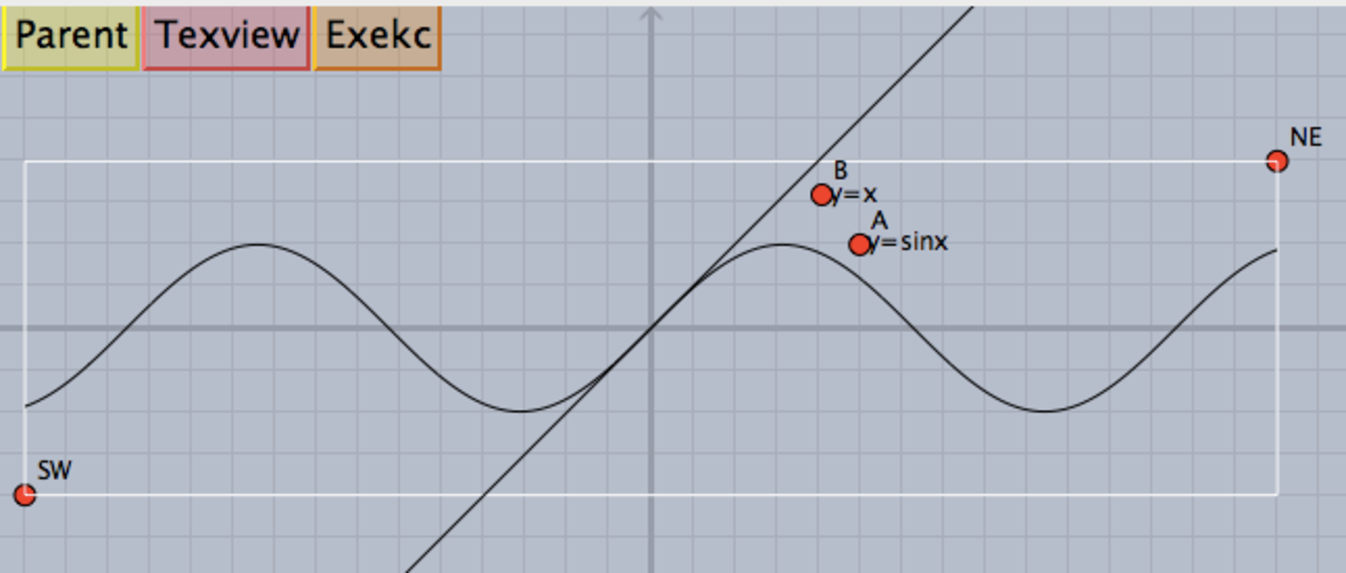
\includegraphics[bb=0.00 0.00 646.00 275.00,height=28mm]{fig/displayscreen.pdf}}
\putnotese{73}{5}{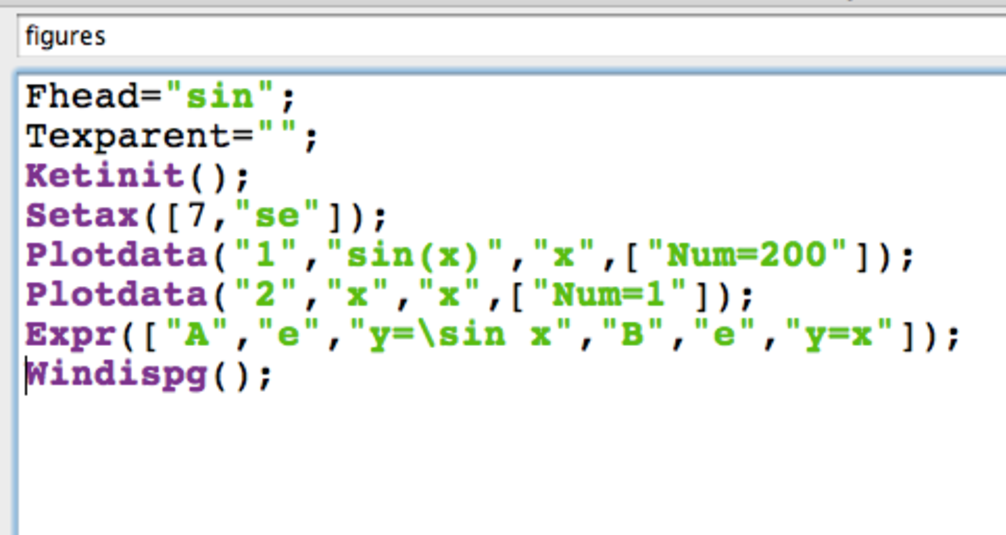
\includegraphics[bb=0.00 0.00 483.00 257.00,height=28mm]{fig/CindyScript.pdf}}
\putnotes{75}{38}{Figure \thefigno\ \ Screens of Cinderella}\addtocounter{figno}{1}%
\end{layer}

\vspace{45mm}

\newpage

So far, \ketcindy\ can generate various types of figures or tables as follows.

\begin{layer}{150}{0}
\putnotes{35}{3}{%%% s106bowhatch.tex 2016-4-23 11:59
%%% s106bowhatch.sce 2016-4-23 11:59
{\unitlength=5mm%
\begin{picture}%
(   9.04000,   7.62000)(  -4.50000,  -4.00000)%
\special{pn 8}%
%
\special{pa -787 591}\special{pa 197 -591}\special{pa 787 591}\special{pa -787 591}%
\special{fp}%
\special{pa 528 171}\special{pa 525 118}\special{pa 515 67}\special{pa 499 16}\special{pa 476 -31}%
\special{pa 448 -76}\special{pa 414 -116}\special{pa 376 -152}\special{pa 333 -183}%
\special{pa 287 -209}\special{pa 238 -228}\special{pa 187 -241}\special{pa 135 -248}%
\special{pa 82 -248}\special{pa 30 -241}\special{pa -21 -228}\special{pa -70 -209}%
\special{pa -116 -183}\special{pa -159 -152}\special{pa -197 -116}\special{pa -231 -76}%
\special{pa -259 -31}\special{pa -282 16}\special{pa -298 67}\special{pa -308 118}%
\special{pa -311 171}\special{pa -308 224}\special{pa -298 275}\special{pa -282 325}%
\special{pa -259 373}\special{pa -231 418}\special{pa -197 458}\special{pa -159 494}%
\special{pa -116 525}\special{pa -70 551}\special{pa -21 570}\special{pa 30 583}\special{pa 82 590}%
\special{pa 135 590}\special{pa 187 583}\special{pa 238 570}\special{pa 287 551}\special{pa 333 525}%
\special{pa 376 494}\special{pa 414 458}\special{pa 448 418}\special{pa 476 373}\special{pa 499 325}%
\special{pa 515 275}\special{pa 525 224}\special{pa 528 171}%
\special{fp}%
\settowidth{\Width}{$c$}\setlength{\Width}{-0.5\Width}%
\settoheight{\Height}{$c$}\settodepth{\Depth}{$c$}\setlength{\Height}{-0.5\Height}\setlength{\Depth}{0.5\Depth}\addtolength{\Height}{\Depth}%
\put(-2.1000,0.5000){\hspace*{\Width}\raisebox{\Height}{$c$}}%
%
%
\special{pa 197 -591}\special{pa 184 -584}\special{pa 171 -577}\special{pa 163 -572}\special{fp}%
\special{pa 129 -553}\special{pa 119 -548}\special{pa 106 -540}\special{pa 95 -533}\special{fp}%
\special{pa 62 -513}\special{pa 56 -509}\special{pa 43 -501}\special{pa 31 -493}\special{pa 29 -492}\special{fp}%
\special{pa -3 -471}\special{pa -6 -469}\special{pa -18 -460}\special{pa -30 -452}\special{pa -35 -448}\special{fp}%
\special{pa -67 -425}\special{pa -78 -417}\special{pa -90 -408}\special{pa -98 -402}\special{fp}%
\special{pa -129 -378}\special{pa -137 -372}\special{pa -148 -362}\special{pa -159 -353}\special{fp}%
\special{pa -188 -328}\special{pa -193 -324}\special{pa -204 -314}\special{pa -215 -304}\special{pa -218 -302}\special{fp}%
\special{pa -246 -276}\special{pa -248 -274}\special{pa -259 -264}\special{pa -269 -254}\special{pa -274 -249}\special{fp}%
\special{pa -302 -221}\special{pa -311 -212}\special{pa -321 -201}\special{pa -329 -193}\special{fp}%
\special{pa -355 -165}\special{pa -362 -158}\special{pa -372 -147}\special{pa -381 -136}\special{fp}%
\special{pa -444 -60}\special{pa -454 -49}\special{pa -463 -37}\special{pa -468 -29}\special{fp}%
\special{pa -492 2}\special{pa -498 11}\special{pa -507 23}\special{pa -514 33}\special{fp}%
\special{pa -536 65}\special{pa -540 71}\special{pa -548 84}\special{pa -556 96}\special{pa -558 98}\special{fp}%
\special{pa -579 131}\special{pa -580 134}\special{pa -588 146}\special{pa -595 159}\special{pa -599 164}\special{fp}%
\special{pa -618 198}\special{pa -625 210}\special{pa -632 223}\special{pa -637 232}\special{fp}%
\special{pa -655 267}\special{pa -660 276}\special{pa -666 289}\special{pa -673 301}\special{fp}%
\special{pa -689 336}\special{pa -692 342}\special{pa -698 356}\special{pa -704 369}\special{pa -705 372}\special{fp}%
\special{pa -721 408}\special{pa -722 410}\special{pa -727 423}\special{pa -733 437}\special{pa -736 444}\special{fp}%
\special{pa -750 480}\special{pa -754 492}\special{pa -759 506}\special{pa -763 517}\special{fp}%
\special{pa -776 553}\special{pa -778 562}\special{pa -783 576}\special{pa -787 591}\special{fp}%
%
%
\settowidth{\Width}{$a$}\setlength{\Width}{-0.5\Width}%
\settoheight{\Height}{$a$}\settodepth{\Depth}{$a$}\setlength{\Height}{-0.5\Height}\setlength{\Depth}{0.5\Depth}\addtolength{\Height}{\Depth}%
\put(3.1000,0.3000){\hspace*{\Width}\raisebox{\Height}{$a$}}%
%
%
\special{pa 787 591}\special{pa 786 578}\special{pa 785 565}\special{pa 784 554}\special{fp}%
\special{pa 781 517}\special{pa 781 515}\special{pa 779 503}\special{pa 778 490}\special{pa 776 480}\special{fp}%
\special{pa 771 444}\special{pa 770 441}\special{pa 768 428}\special{pa 766 416}\special{pa 765 407}\special{fp}%
\special{pa 758 371}\special{pa 757 367}\special{pa 754 354}\special{pa 752 342}\special{pa 750 335}\special{fp}%
\special{pa 742 299}\special{pa 740 293}\special{pa 737 281}\special{pa 734 269}\special{pa 733 263}\special{fp}%
\special{pa 723 227}\special{pa 721 220}\special{pa 717 208}\special{pa 713 196}\special{pa 712 192}\special{fp}%
\special{pa 700 157}\special{pa 697 148}\special{pa 693 137}\special{pa 689 125}\special{pa 688 122}\special{fp}%
\special{pa 675 87}\special{pa 671 78}\special{pa 667 66}\special{pa 662 54}\special{pa 661 53}\special{fp}%
\special{pa 647 19}\special{pa 642 8}\special{pa 637 -3}\special{pa 632 -15}\special{fp}%
\special{pa 588 -103}\special{pa 582 -114}\special{pa 576 -125}\special{pa 570 -135}\special{fp}%
\special{pa 551 -167}\special{pa 551 -168}\special{pa 544 -179}\special{pa 537 -190}\special{pa 532 -199}\special{fp}%
\special{pa 512 -230}\special{pa 511 -232}\special{pa 504 -243}\special{pa 497 -253}\special{pa 492 -261}\special{fp}%
\special{pa 470 -291}\special{pa 468 -295}\special{pa 460 -305}\special{pa 453 -315}\special{pa 449 -321}\special{fp}%
\special{pa 426 -350}\special{pa 422 -355}\special{pa 415 -365}\special{pa 407 -374}\special{pa 403 -379}\special{fp}%
\special{pa 379 -407}\special{pa 374 -413}\special{pa 366 -422}\special{pa 358 -432}\special{pa 355 -435}\special{fp}%
\special{pa 330 -462}\special{pa 324 -469}\special{pa 315 -478}\special{pa 307 -487}\special{pa 304 -489}\special{fp}%
\special{pa 278 -515}\special{pa 271 -523}\special{pa 262 -531}\special{pa 253 -540}\special{pa 252 -541}\special{fp}%
\special{pa 225 -566}\special{pa 216 -574}\special{pa 206 -582}\special{pa 197 -591}\special{fp}%
%
%
\settowidth{\Width}{$b$}\setlength{\Width}{-0.5\Width}%
\settoheight{\Height}{$b$}\settodepth{\Depth}{$b$}\setlength{\Height}{-0.5\Height}\setlength{\Depth}{0.5\Depth}\addtolength{\Height}{\Depth}%
\put(0.0000,-3.8000){\hspace*{\Width}\raisebox{\Height}{$b$}}%
%
%
\special{pa -787 591}\special{pa -773 596}\special{pa -759 602}\special{pa -754 604}\special{fp}%
\special{pa -720 617}\special{pa -717 618}\special{pa -703 624}\special{pa -688 629}\special{pa -686 630}\special{fp}%
\special{pa -652 641}\special{pa -645 644}\special{pa -631 648}\special{pa -618 653}\special{fp}%
\special{pa -583 663}\special{pa -573 666}\special{pa -558 670}\special{pa -548 673}\special{fp}%
\special{pa -514 683}\special{pa -500 686}\special{pa -485 690}\special{pa -478 691}\special{fp}%
\special{pa -443 699}\special{pa -440 700}\special{pa -426 703}\special{pa -411 706}\special{pa -408 707}\special{fp}%
\special{pa -372 714}\special{pa -366 715}\special{pa -351 718}\special{pa -337 720}\special{fp}%
\special{pa -301 726}\special{pa -291 727}\special{pa -276 729}\special{pa -265 731}\special{fp}%
\special{pa -229 735}\special{pa -216 737}\special{pa -201 738}\special{pa -193 739}\special{fp}%
\special{pa -157 742}\special{pa -155 742}\special{pa -140 743}\special{pa -125 744}\special{pa -121 744}\special{fp}%
\special{pa -85 746}\special{pa -80 746}\special{pa -64 747}\special{pa -49 747}\special{fp}%
\special{pa 49 747}\special{pa 64 747}\special{pa 80 746}\special{pa 85 746}\special{fp}%
\special{pa 121 744}\special{pa 125 744}\special{pa 140 743}\special{pa 155 742}\special{pa 157 742}\special{fp}%
\special{pa 193 739}\special{pa 201 738}\special{pa 216 737}\special{pa 229 735}\special{fp}%
\special{pa 265 731}\special{pa 276 729}\special{pa 291 727}\special{pa 301 726}\special{fp}%
\special{pa 337 720}\special{pa 351 718}\special{pa 366 715}\special{pa 372 714}\special{fp}%
\special{pa 408 707}\special{pa 411 706}\special{pa 426 703}\special{pa 440 700}\special{pa 443 699}\special{fp}%
\special{pa 478 691}\special{pa 485 690}\special{pa 500 686}\special{pa 514 683}\special{fp}%
\special{pa 548 673}\special{pa 558 670}\special{pa 573 666}\special{pa 583 663}\special{fp}%
\special{pa 618 653}\special{pa 631 648}\special{pa 645 644}\special{pa 652 641}\special{fp}%
\special{pa 686 630}\special{pa 688 629}\special{pa 703 624}\special{pa 717 618}\special{pa 720 617}\special{fp}%
\special{pa 754 604}\special{pa 759 602}\special{pa 773 596}\special{pa 787 591}\special{fp}%
%
%
\special{pn 6}%
\special{pa 732 591}\special{pa 769 553}%
\special{fp}%
\special{pa 662 591}\special{pa 746 507}%
\special{fp}%
\special{pa 593 591}\special{pa 722 461}%
\special{fp}%
\special{pa 523 591}\special{pa 699 414}%
\special{fp}%
\special{pa 453 591}\special{pa 676 368}%
\special{fp}%
\special{pa 384 591}\special{pa 653 321}%
\special{fp}%
\special{pa 314 591}\special{pa 630 275}%
\special{fp}%
\special{pa 245 591}\special{pa 283 552}%
\special{fp}%
\special{pa 489 346}\special{pa 606 229}%
\special{fp}%
\special{pa 175 591}\special{pa 182 584}%
\special{fp}%
\special{pa 521 245}\special{pa 583 182}%
\special{fp}%
\special{pa 105 591}\special{pa 106 590}%
\special{fp}%
\special{pa 528 168}\special{pa 560 136}%
\special{fp}%
\special{pa 36 591}\special{pa 42 585}%
\special{fp}%
\special{pa 522 104}\special{pa 537 90}%
\special{fp}%
\special{pa -34 591}\special{pa -15 572}%
\special{fp}%
\special{pa 509 48}\special{pa 514 43}%
\special{fp}%
\special{pa -103 591}\special{pa -65 553}%
\special{fp}%
\special{pa 490 -3}\special{pa 490 -3}%
\special{fp}%
\special{pa -173 591}\special{pa -111 528}%
\special{fp}%
\special{pa 466 -48}\special{pa 467 -50}%
\special{fp}%
\special{pa -243 591}\special{pa -152 500}%
\special{fp}%
\special{pa 437 -89}\special{pa 444 -96}%
\special{fp}%
\special{pa -312 591}\special{pa -188 467}%
\special{fp}%
\special{pa 404 -126}\special{pa 421 -143}%
\special{fp}%
\special{pa -382 591}\special{pa -221 430}%
\special{fp}%
\special{pa 367 -159}\special{pa 398 -189}%
\special{fp}%
\special{pa -451 591}\special{pa -249 389}%
\special{fp}%
\special{pa 326 -187}\special{pa 374 -235}%
\special{fp}%
\special{pa -521 591}\special{pa -273 343}%
\special{fp}%
\special{pa 281 -211}\special{pa 351 -282}%
\special{fp}%
\special{pa -591 591}\special{pa -292 292}%
\special{fp}%
\special{pa 230 -230}\special{pa 328 -328}%
\special{fp}%
\special{pa -660 591}\special{pa -305 236}%
\special{fp}%
\special{pa 173 -243}\special{pa 305 -374}%
\special{fp}%
\special{pa -730 591}\special{pa -311 172}%
\special{fp}%
\special{pa 109 -248}\special{pa 282 -421}%
\special{fp}%
\special{pa -728 519}\special{pa -303 94}%
\special{fp}%
\special{pa 33 -242}\special{pa 258 -467}%
\special{fp}%
\special{pa -380 101}\special{pa -270 -8}%
\special{fp}%
\special{pa -69 -209}\special{pa 235 -514}%
\special{fp}%
\special{pa -32 -316}\special{pa 212 -560}%
\special{fp}%
\special{pn 8}%
\special{pn 4}%
\special{pa 120 160}\special{pa 113 156}\special{pa 104 156}\special{pa 97 160}\special{pa 93 167}%
\special{pa 93 175}\special{pa 97 182}\special{pa 104 186}\special{pa 113 186}\special{pa 120 182}%
\special{pa 124 175}\special{pa 124 167}\special{pa 120 160}\special{sh 1}\special{fp}%
\special{pn 8}%
\settowidth{\Width}{A}\setlength{\Width}{-1\Width}%
\settoheight{\Height}{A}\settodepth{\Depth}{A}\setlength{\Height}{-\Height}%
\put(-4.0500,-3.0500){\hspace*{\Width}\raisebox{\Height}{A}}%
%
%
\settowidth{\Width}{B}\setlength{\Width}{0\Width}%
\settoheight{\Height}{B}\settodepth{\Depth}{B}\setlength{\Height}{\Depth}%
\put(1.0500,3.0500){\hspace*{\Width}\raisebox{\Height}{B}}%
%
%
\settowidth{\Width}{C}\setlength{\Width}{0\Width}%
\settoheight{\Height}{C}\settodepth{\Depth}{C}\setlength{\Height}{-\Height}%
\put(4.0500,-3.0500){\hspace*{\Width}\raisebox{\Height}{C}}%
%
%
\settowidth{\Width}{I}\setlength{\Width}{0\Width}%
\settoheight{\Height}{I}\settodepth{\Depth}{I}\setlength{\Height}{-\Height}%
\put(0.6010,-0.9184){\hspace*{\Width}\raisebox{\Height}{I}}%
%
%
\end{picture}}%}
\putnotes{35}{46}{Figure \thefigno\ \ Geometric Figure}\addtocounter{figno}{1}%
\putnotes{95}{6}{%%% s210diffeq2.tex 2016-4-23 12:4
%%% s210diffeq2.sce 2016-4-23 12:4
{\unitlength=5mm%
\begin{picture}%
(   9.68000,   8.11000)(  -0.65000,  -3.59000)%
\special{pn 8}%
%
\special{pa 0 -787}\special{pa 9 -783}\special{pa 18 -769}\special{pa 27 -747}\special{pa 36 -717}%
\special{pa 44 -679}\special{pa 53 -634}\special{pa 62 -582}\special{pa 71 -524}\special{pa 80 -462}%
\special{pa 89 -395}\special{pa 98 -325}\special{pa 107 -252}\special{pa 116 -178}%
\special{pa 124 -103}\special{pa 133 -28}\special{pa 142 45}\special{pa 151 117}\special{pa 160 187}%
\special{pa 169 253}\special{pa 178 314}\special{pa 187 372}\special{pa 196 423}\special{pa 204 469}%
\special{pa 213 509}\special{pa 222 542}\special{pa 231 569}\special{pa 240 588}\special{pa 249 600}%
\special{pa 258 605}\special{pa 267 603}\special{pa 276 594}\special{pa 284 578}\special{pa 293 556}%
\special{pa 302 528}\special{pa 311 495}\special{pa 320 456}\special{pa 329 412}\special{pa 338 365}%
\special{pa 347 314}\special{pa 356 261}\special{pa 364 206}\special{pa 373 149}\special{pa 382 91}%
\special{pa 391 34}\special{pa 400 -23}\special{pa 409 -79}\special{pa 418 -133}\special{pa 427 -184}%
\special{pa 436 -232}\special{pa 444 -277}\special{pa 453 -317}\special{pa 462 -354}%
\special{pa 471 -385}\special{pa 480 -412}\special{pa 489 -433}\special{pa 498 -449}%
\special{pa 507 -460}\special{pa 515 -465}\special{pa 524 -464}\special{pa 533 -458}%
\special{pa 542 -447}\special{pa 551 -431}\special{pa 560 -411}\special{pa 569 -386}%
\special{pa 578 -357}\special{pa 587 -324}\special{pa 595 -288}\special{pa 604 -250}%
\special{pa 613 -209}\special{pa 622 -167}\special{pa 631 -123}\special{pa 640 -79}%
\special{pa 649 -35}\special{pa 658 9}\special{pa 667 52}\special{pa 675 93}\special{pa 684 133}%
\special{pa 693 171}\special{pa 702 206}\special{pa 711 238}\special{pa 720 266}\special{pa 729 291}%
\special{pa 738 313}\special{pa 747 330}\special{pa 755 343}\special{pa 764 352}\special{pa 773 357}%
\special{pa 782 357}\special{pa 791 354}\special{pa 800 346}\special{pa 809 334}\special{pa 818 319}%
\special{pa 827 301}\special{pa 835 279}\special{pa 844 255}\special{pa 853 228}\special{pa 862 198}%
\special{pa 871 167}\special{pa 880 135}\special{pa 889 102}\special{pa 898 68}\special{pa 907 34}%
\special{pa 915 0}\special{pa 924 -33}\special{pa 933 -65}\special{pa 942 -96}\special{pa 951 -125}%
\special{pa 960 -153}\special{pa 969 -178}\special{pa 978 -200}\special{pa 987 -220}%
\special{pa 995 -237}\special{pa 1004 -251}\special{pa 1013 -262}\special{pa 1022 -269}%
\special{pa 1031 -274}\special{pa 1040 -275}\special{pa 1049 -273}\special{pa 1058 -267}%
\special{pa 1067 -259}\special{pa 1075 -248}\special{pa 1084 -234}\special{pa 1093 -218}%
\special{pa 1102 -200}\special{pa 1111 -179}\special{pa 1120 -157}\special{pa 1129 -134}%
\special{pa 1138 -109}\special{pa 1147 -84}\special{pa 1155 -58}\special{pa 1164 -32}%
\special{pa 1173 -6}\special{pa 1182 20}\special{pa 1191 45}\special{pa 1200 69}\special{pa 1209 92}%
\special{pa 1218 113}\special{pa 1227 133}\special{pa 1235 151}\special{pa 1244 166}%
\special{pa 1253 180}\special{pa 1262 191}\special{pa 1271 200}\special{pa 1280 206}%
\special{pa 1289 210}\special{pa 1298 211}\special{pa 1307 210}\special{pa 1315 206}%
\special{pa 1324 201}\special{pa 1333 193}\special{pa 1342 182}\special{pa 1351 170}%
\special{pa 1360 157}\special{pa 1369 141}\special{pa 1378 124}\special{pa 1386 107}%
\special{pa 1395 88}\special{pa 1404 68}\special{pa 1413 49}\special{pa 1422 28}\special{pa 1431 8}%
\special{pa 1440 -11}\special{pa 1449 -31}\special{pa 1458 -49}\special{pa 1466 -67}%
\special{pa 1475 -84}\special{pa 1484 -99}\special{pa 1493 -113}\special{pa 1502 -125}%
\special{pa 1511 -136}\special{pa 1520 -145}\special{pa 1529 -152}\special{pa 1538 -157}%
\special{pa 1546 -161}\special{pa 1555 -162}\special{pa 1564 -162}\special{pa 1573 -159}%
\special{pa 1582 -155}\special{pa 1591 -149}\special{pa 1600 -142}\special{pa 1609 -133}%
\special{pa 1618 -123}\special{pa 1626 -111}\special{pa 1635 -98}\special{pa 1644 -85}%
\special{pa 1653 -71}\special{pa 1662 -56}\special{pa 1671 -41}\special{pa 1680 -25}%
\special{pa 1689 -10}\special{pa 1698 6}\special{pa 1706 21}\special{pa 1715 35}\special{pa 1724 49}%
\special{pa 1733 62}\special{pa 1742 74}\special{pa 1751 85}\special{pa 1760 94}\special{pa 1769 103}%
\special{pa 1778 110}%
\special{fp}%
\settowidth{\Width}{$\displaystyle\frac{d^2 x}{dt^2}+0.4\displaystyle\frac{dx}{dt}+5.71x=0$}\setlength{\Width}{0\Width}%
\settoheight{\Height}{$\displaystyle\frac{d^2 x}{dt^2}+0.4\displaystyle\frac{dx}{dt}+5.71x=0$}\settodepth{\Depth}{$\displaystyle\frac{d^2 x}{dt^2}+0.4\displaystyle\frac{dx}{dt}+5.71x=0$}\setlength{\Height}{-0.5\Height}\setlength{\Depth}{0.5\Depth}\addtolength{\Height}{\Depth}%
\put(2.0500,4.0000){\hspace*{\Width}\raisebox{\Height}{$\displaystyle\frac{d^2 x}{dt^2}+0.4\displaystyle\frac{dx}{dt}+5.71x=0$}}%
%
%
\special{pa -128 0}\special{pa 1778 0}%
\special{fp}%
\special{pa 0 707}\special{pa 0 -890}%
\special{fp}%
\settowidth{\Width}{$x$}\setlength{\Width}{0\Width}%
\settoheight{\Height}{$x$}\settodepth{\Depth}{$x$}\setlength{\Height}{-0.5\Height}\setlength{\Depth}{0.5\Depth}\addtolength{\Height}{\Depth}%
\put(9.0800,0.0000){\hspace*{\Width}\raisebox{\Height}{$x$}}%
%
%
\settowidth{\Width}{$y$}\setlength{\Width}{-0.5\Width}%
\settoheight{\Height}{$y$}\settodepth{\Depth}{$y$}\setlength{\Height}{\Depth}%
\put(0.0000,4.5700){\hspace*{\Width}\raisebox{\Height}{$y$}}%
%
%
\settowidth{\Width}{O}\setlength{\Width}{-1\Width}%
\settoheight{\Height}{O}\settodepth{\Depth}{O}\setlength{\Height}{-\Height}%
\put(-0.0500,-0.0500){\hspace*{\Width}\raisebox{\Height}{O}}%
%
%
\end{picture}}%}
\putnotes{105}{46}{Figure \thefigno\ \ Graph of Function}\addtocounter{figno}{1}%
\putnotes{35}{53}{%%% s305incanddec.tex 2016-4-24 19:53
%%% s305incanddec.sce 2016-4-24 19:53
{\unitlength=5mm%
\begin{picture}%
(  11.41000,  11.00000)(  -0.00000,   1.00000)%
\special{pn 8}%
%
\special{pa 0 -2362}\special{pa 0 -197}%
\special{fp}%
\special{pa 2246 -2362}\special{pa 2246 -197}%
\special{fp}%
\special{pa 0 -2362}\special{pa 2246 -2362}%
\special{fp}%
\special{pa 0 -2165}\special{pa 2246 -2165}%
\special{fp}%
\special{pa 0 -1969}\special{pa 2246 -1969}%
\special{fp}%
\special{pa 0 -1772}\special{pa 2246 -1772}%
\special{fp}%
\special{pa 0 -1575}\special{pa 2246 -1575}%
\special{fp}%
\special{pa 0 -197}\special{pa 2246 -197}%
\special{fp}%
\special{pa 295 -2362}\special{pa 295 -1575}%
\special{fp}%
\special{pa 591 -2362}\special{pa 591 -1575}%
\special{fp}%
\special{pa 943 -2362}\special{pa 943 -1575}%
\special{fp}%
\special{pa 1238 -2362}\special{pa 1238 -1575}%
\special{fp}%
\special{pa 1593 -2362}\special{pa 1593 -1575}%
\special{fp}%
\special{pa 1892 -2362}\special{pa 1892 -1575}%
\special{fp}%
\special{pa 295 -2165}\special{pa 591 -1575}%
\special{fp}%
\special{pa 591 -2165}\special{pa 295 -1575}%
\special{fp}%
\scriptsize%
\settowidth{\Width}{$x$}\setlength{\Width}{-0.5\Width}%
\settoheight{\Height}{$x$}\settodepth{\Depth}{$x$}\setlength{\Height}{-0.5\Height}\setlength{\Depth}{0.5\Depth}\addtolength{\Height}{\Depth}%
\put(0.7500,11.5000){\hspace*{\Width}\raisebox{\Height}{$x$}}%
%
%
\settowidth{\Width}{$0$}\setlength{\Width}{-0.5\Width}%
\settoheight{\Height}{$0$}\settodepth{\Depth}{$0$}\setlength{\Height}{-0.5\Height}\setlength{\Depth}{0.5\Depth}\addtolength{\Height}{\Depth}%
\put(2.2500,11.5000){\hspace*{\Width}\raisebox{\Height}{$0$}}%
%
%
\settowidth{\Width}{$\cdots$}\setlength{\Width}{-0.5\Width}%
\settoheight{\Height}{$\cdots$}\settodepth{\Depth}{$\cdots$}\setlength{\Height}{-0.5\Height}\setlength{\Depth}{0.5\Depth}\addtolength{\Height}{\Depth}%
\put(3.8950,11.5000){\hspace*{\Width}\raisebox{\Height}{$\cdots$}}%
%
%
\settowidth{\Width}{$e$}\setlength{\Width}{-0.5\Width}%
\settoheight{\Height}{$e$}\settodepth{\Depth}{$e$}\setlength{\Height}{-0.5\Height}\setlength{\Depth}{0.5\Depth}\addtolength{\Height}{\Depth}%
\put(5.5400,11.5000){\hspace*{\Width}\raisebox{\Height}{$e$}}%
%
%
\settowidth{\Width}{$\cdots$}\setlength{\Width}{-0.5\Width}%
\settoheight{\Height}{$\cdots$}\settodepth{\Depth}{$\cdots$}\setlength{\Height}{-0.5\Height}\setlength{\Depth}{0.5\Depth}\addtolength{\Height}{\Depth}%
\put(7.1900,11.5000){\hspace*{\Width}\raisebox{\Height}{$\cdots$}}%
%
%
\settowidth{\Width}{$e\sqrt{e}$}\setlength{\Width}{-0.5\Width}%
\settoheight{\Height}{$e\sqrt{e}$}\settodepth{\Depth}{$e\sqrt{e}$}\setlength{\Height}{-0.5\Height}\setlength{\Depth}{0.5\Depth}\addtolength{\Height}{\Depth}%
\put(8.8500,11.5000){\hspace*{\Width}\raisebox{\Height}{$e\sqrt{e}$}}%
%
%
\settowidth{\Width}{$\cdots$}\setlength{\Width}{-0.5\Width}%
\settoheight{\Height}{$\cdots$}\settodepth{\Depth}{$\cdots$}\setlength{\Height}{-0.5\Height}\setlength{\Depth}{0.5\Depth}\addtolength{\Height}{\Depth}%
\put(10.5100,11.5000){\hspace*{\Width}\raisebox{\Height}{$\cdots$}}%
%
%
\settowidth{\Width}{$y'$}\setlength{\Width}{-0.5\Width}%
\settoheight{\Height}{$y'$}\settodepth{\Depth}{$y'$}\setlength{\Height}{-0.5\Height}\setlength{\Depth}{0.5\Depth}\addtolength{\Height}{\Depth}%
\put(0.7500,10.5000){\hspace*{\Width}\raisebox{\Height}{$y'$}}%
%
%
\settowidth{\Width}{$$}\setlength{\Width}{-0.5\Width}%
\settoheight{\Height}{$$}\settodepth{\Depth}{$$}\setlength{\Height}{-0.5\Height}\setlength{\Depth}{0.5\Depth}\addtolength{\Height}{\Depth}%
\put(2.2500,10.5000){\hspace*{\Width}\raisebox{\Height}{$$}}%
%
%
\settowidth{\Width}{$+$}\setlength{\Width}{-0.5\Width}%
\settoheight{\Height}{$+$}\settodepth{\Depth}{$+$}\setlength{\Height}{-0.5\Height}\setlength{\Depth}{0.5\Depth}\addtolength{\Height}{\Depth}%
\put(3.8950,10.5000){\hspace*{\Width}\raisebox{\Height}{$+$}}%
%
%
\settowidth{\Width}{$0$}\setlength{\Width}{-0.5\Width}%
\settoheight{\Height}{$0$}\settodepth{\Depth}{$0$}\setlength{\Height}{-0.5\Height}\setlength{\Depth}{0.5\Depth}\addtolength{\Height}{\Depth}%
\put(5.5400,10.5000){\hspace*{\Width}\raisebox{\Height}{$0$}}%
%
%
\settowidth{\Width}{$-$}\setlength{\Width}{-0.5\Width}%
\settoheight{\Height}{$-$}\settodepth{\Depth}{$-$}\setlength{\Height}{-0.5\Height}\setlength{\Depth}{0.5\Depth}\addtolength{\Height}{\Depth}%
\put(7.1900,10.5000){\hspace*{\Width}\raisebox{\Height}{$-$}}%
%
%
\settowidth{\Width}{$-$}\setlength{\Width}{-0.5\Width}%
\settoheight{\Height}{$-$}\settodepth{\Depth}{$-$}\setlength{\Height}{-0.5\Height}\setlength{\Depth}{0.5\Depth}\addtolength{\Height}{\Depth}%
\put(8.8500,10.5000){\hspace*{\Width}\raisebox{\Height}{$-$}}%
%
%
\settowidth{\Width}{$-$}\setlength{\Width}{-0.5\Width}%
\settoheight{\Height}{$-$}\settodepth{\Depth}{$-$}\setlength{\Height}{-0.5\Height}\setlength{\Depth}{0.5\Depth}\addtolength{\Height}{\Depth}%
\put(10.5100,10.5000){\hspace*{\Width}\raisebox{\Height}{$-$}}%
%
%
\settowidth{\Width}{$y''$}\setlength{\Width}{-0.5\Width}%
\settoheight{\Height}{$y''$}\settodepth{\Depth}{$y''$}\setlength{\Height}{-0.5\Height}\setlength{\Depth}{0.5\Depth}\addtolength{\Height}{\Depth}%
\put(0.7500,9.5000){\hspace*{\Width}\raisebox{\Height}{$y''$}}%
%
%
\settowidth{\Width}{$$}\setlength{\Width}{-0.5\Width}%
\settoheight{\Height}{$$}\settodepth{\Depth}{$$}\setlength{\Height}{-0.5\Height}\setlength{\Depth}{0.5\Depth}\addtolength{\Height}{\Depth}%
\put(2.2500,9.5000){\hspace*{\Width}\raisebox{\Height}{$$}}%
%
%
\settowidth{\Width}{$-$}\setlength{\Width}{-0.5\Width}%
\settoheight{\Height}{$-$}\settodepth{\Depth}{$-$}\setlength{\Height}{-0.5\Height}\setlength{\Depth}{0.5\Depth}\addtolength{\Height}{\Depth}%
\put(3.8950,9.5000){\hspace*{\Width}\raisebox{\Height}{$-$}}%
%
%
\settowidth{\Width}{$-$}\setlength{\Width}{-0.5\Width}%
\settoheight{\Height}{$-$}\settodepth{\Depth}{$-$}\setlength{\Height}{-0.5\Height}\setlength{\Depth}{0.5\Depth}\addtolength{\Height}{\Depth}%
\put(5.5400,9.5000){\hspace*{\Width}\raisebox{\Height}{$-$}}%
%
%
\settowidth{\Width}{$-$}\setlength{\Width}{-0.5\Width}%
\settoheight{\Height}{$-$}\settodepth{\Depth}{$-$}\setlength{\Height}{-0.5\Height}\setlength{\Depth}{0.5\Depth}\addtolength{\Height}{\Depth}%
\put(7.1900,9.5000){\hspace*{\Width}\raisebox{\Height}{$-$}}%
%
%
\settowidth{\Width}{$0$}\setlength{\Width}{-0.5\Width}%
\settoheight{\Height}{$0$}\settodepth{\Depth}{$0$}\setlength{\Height}{-0.5\Height}\setlength{\Depth}{0.5\Depth}\addtolength{\Height}{\Depth}%
\put(8.8500,9.5000){\hspace*{\Width}\raisebox{\Height}{$0$}}%
%
%
\settowidth{\Width}{$+$}\setlength{\Width}{-0.5\Width}%
\settoheight{\Height}{$+$}\settodepth{\Depth}{$+$}\setlength{\Height}{-0.5\Height}\setlength{\Depth}{0.5\Depth}\addtolength{\Height}{\Depth}%
\put(10.5100,9.5000){\hspace*{\Width}\raisebox{\Height}{$+$}}%
%
%
\settowidth{\Width}{$y$}\setlength{\Width}{-0.5\Width}%
\settoheight{\Height}{$y$}\settodepth{\Depth}{$y$}\setlength{\Height}{-0.5\Height}\setlength{\Depth}{0.5\Depth}\addtolength{\Height}{\Depth}%
\put(0.7500,8.5000){\hspace*{\Width}\raisebox{\Height}{$y$}}%
%
%
\settowidth{\Width}{$$}\setlength{\Width}{-0.5\Width}%
\settoheight{\Height}{$$}\settodepth{\Depth}{$$}\setlength{\Height}{-0.5\Height}\setlength{\Depth}{0.5\Depth}\addtolength{\Height}{\Depth}%
\put(2.2500,8.5000){\hspace*{\Width}\raisebox{\Height}{$$}}%
%
%
\settowidth{\Width}{$$}\setlength{\Width}{-0.5\Width}%
\settoheight{\Height}{$$}\settodepth{\Depth}{$$}\setlength{\Height}{-0.5\Height}\setlength{\Depth}{0.5\Depth}\addtolength{\Height}{\Depth}%
\put(3.8950,8.5000){\hspace*{\Width}\raisebox{\Height}{$$}}%
%
%
\settowidth{\Width}{$\frac{10}{e}$}\setlength{\Width}{-0.5\Width}%
\settoheight{\Height}{$\frac{10}{e}$}\settodepth{\Depth}{$\frac{10}{e}$}\setlength{\Height}{-0.5\Height}\setlength{\Depth}{0.5\Depth}\addtolength{\Height}{\Depth}%
\put(5.5400,8.5000){\hspace*{\Width}\raisebox{\Height}{$\frac{10}{e}$}}%
%
%
\settowidth{\Width}{$$}\setlength{\Width}{-0.5\Width}%
\settoheight{\Height}{$$}\settodepth{\Depth}{$$}\setlength{\Height}{-0.5\Height}\setlength{\Depth}{0.5\Depth}\addtolength{\Height}{\Depth}%
\put(7.1900,8.5000){\hspace*{\Width}\raisebox{\Height}{$$}}%
%
%
\settowidth{\Width}{$\frac{15}{e\sqrt{e}}$}\setlength{\Width}{-0.5\Width}%
\settoheight{\Height}{$\frac{15}{e\sqrt{e}}$}\settodepth{\Depth}{$\frac{15}{e\sqrt{e}}$}\setlength{\Height}{-0.5\Height}\setlength{\Depth}{0.5\Depth}\addtolength{\Height}{\Depth}%
\put(8.8500,8.5000){\hspace*{\Width}\raisebox{\Height}{$\frac{15}{e\sqrt{e}}$}}%
%
%
\settowidth{\Width}{$$}\setlength{\Width}{-0.5\Width}%
\settoheight{\Height}{$$}\settodepth{\Depth}{$$}\setlength{\Height}{-0.5\Height}\setlength{\Depth}{0.5\Depth}\addtolength{\Height}{\Depth}%
\put(10.5100,8.5000){\hspace*{\Width}\raisebox{\Height}{$$}}%
%
%
\settowidth{\Width}{%%% s304graphforincanddec.tex 2016-4-23 12:15
%%% s304graphforincanddec.sce 2016-4-23 12:15
{\unitlength=5mm%
\begin{picture}%
(   9.96000,   5.66000)(  -0.65000,  -1.22000)%
\special{pn 8}%
%
\special{pa 177 240}\special{pa 183 151}\special{pa 202 -46}\special{pa 220 -195}%
\special{pa 238 -310}\special{pa 257 -400}\special{pa 275 -471}\special{pa 293 -527}%
\special{pa 312 -571}\special{pa 330 -606}\special{pa 348 -635}\special{pa 367 -657}%
\special{pa 385 -675}\special{pa 403 -689}\special{pa 422 -700}\special{pa 440 -708}%
\special{pa 458 -714}\special{pa 476 -719}\special{pa 495 -722}\special{pa 513 -724}%
\special{pa 531 -724}\special{pa 550 -724}\special{pa 568 -723}\special{pa 586 -721}%
\special{pa 605 -719}\special{pa 623 -717}\special{pa 641 -714}\special{pa 660 -710}%
\special{pa 678 -707}\special{pa 696 -703}\special{pa 715 -699}\special{pa 733 -695}%
\special{pa 751 -691}\special{pa 770 -686}\special{pa 788 -682}\special{pa 806 -678}%
\special{pa 825 -673}\special{pa 843 -669}\special{pa 861 -664}\special{pa 880 -659}%
\special{pa 898 -655}\special{pa 916 -650}\special{pa 935 -646}\special{pa 953 -641}%
\special{pa 971 -637}\special{pa 990 -632}\special{pa 1008 -628}\special{pa 1026 -623}%
\special{pa 1045 -619}\special{pa 1063 -615}\special{pa 1081 -610}\special{pa 1100 -606}%
\special{pa 1118 -602}\special{pa 1136 -598}\special{pa 1155 -594}\special{pa 1173 -590}%
\special{pa 1191 -586}\special{pa 1210 -582}\special{pa 1228 -578}\special{pa 1246 -574}%
\special{pa 1265 -570}\special{pa 1283 -566}\special{pa 1301 -562}\special{pa 1320 -559}%
\special{pa 1338 -555}\special{pa 1356 -551}\special{pa 1375 -548}\special{pa 1393 -544}%
\special{pa 1411 -541}\special{pa 1429 -537}\special{pa 1448 -534}\special{pa 1466 -531}%
\special{pa 1484 -527}\special{pa 1503 -524}\special{pa 1521 -521}\special{pa 1539 -518}%
\special{pa 1558 -515}\special{pa 1576 -511}\special{pa 1594 -508}\special{pa 1613 -505}%
\special{pa 1631 -502}\special{pa 1649 -499}\special{pa 1668 -496}\special{pa 1686 -494}%
\special{pa 1704 -491}\special{pa 1723 -488}\special{pa 1741 -485}\special{pa 1759 -482}%
\special{pa 1778 -480}\special{pa 1796 -477}\special{pa 1814 -474}\special{pa 1833 -472}%
\special{fp}%
\special{pa -128 0}\special{pa 1833 0}%
\special{fp}%
\special{pa 0 240}\special{pa 0 -874}%
\special{fp}%
\settowidth{\Width}{$x$}\setlength{\Width}{0\Width}%
\settoheight{\Height}{$x$}\settodepth{\Depth}{$x$}\setlength{\Height}{-0.5\Height}\setlength{\Depth}{0.5\Depth}\addtolength{\Height}{\Depth}%
\put(9.3600,0.0000){\hspace*{\Width}\raisebox{\Height}{$x$}}%
%
%
\settowidth{\Width}{$y$}\setlength{\Width}{-0.5\Width}%
\settoheight{\Height}{$y$}\settodepth{\Depth}{$y$}\setlength{\Height}{\Depth}%
\put(0.0000,4.4900){\hspace*{\Width}\raisebox{\Height}{$y$}}%
%
%
\settowidth{\Width}{O}\setlength{\Width}{-1\Width}%
\settoheight{\Height}{O}\settodepth{\Depth}{O}\setlength{\Height}{-\Height}%
\put(-0.0500,-0.0500){\hspace*{\Width}\raisebox{\Height}{O}}%
%
%
\end{picture}}%}\setlength{\Width}{-0.5\Width}%
\settoheight{\Height}{%%% s304graphforincanddec.tex 2016-4-23 12:15
%%% s304graphforincanddec.sce 2016-4-23 12:15
{\unitlength=5mm%
\begin{picture}%
(   9.96000,   5.66000)(  -0.65000,  -1.22000)%
\special{pn 8}%
%
\special{pa 177 240}\special{pa 183 151}\special{pa 202 -46}\special{pa 220 -195}%
\special{pa 238 -310}\special{pa 257 -400}\special{pa 275 -471}\special{pa 293 -527}%
\special{pa 312 -571}\special{pa 330 -606}\special{pa 348 -635}\special{pa 367 -657}%
\special{pa 385 -675}\special{pa 403 -689}\special{pa 422 -700}\special{pa 440 -708}%
\special{pa 458 -714}\special{pa 476 -719}\special{pa 495 -722}\special{pa 513 -724}%
\special{pa 531 -724}\special{pa 550 -724}\special{pa 568 -723}\special{pa 586 -721}%
\special{pa 605 -719}\special{pa 623 -717}\special{pa 641 -714}\special{pa 660 -710}%
\special{pa 678 -707}\special{pa 696 -703}\special{pa 715 -699}\special{pa 733 -695}%
\special{pa 751 -691}\special{pa 770 -686}\special{pa 788 -682}\special{pa 806 -678}%
\special{pa 825 -673}\special{pa 843 -669}\special{pa 861 -664}\special{pa 880 -659}%
\special{pa 898 -655}\special{pa 916 -650}\special{pa 935 -646}\special{pa 953 -641}%
\special{pa 971 -637}\special{pa 990 -632}\special{pa 1008 -628}\special{pa 1026 -623}%
\special{pa 1045 -619}\special{pa 1063 -615}\special{pa 1081 -610}\special{pa 1100 -606}%
\special{pa 1118 -602}\special{pa 1136 -598}\special{pa 1155 -594}\special{pa 1173 -590}%
\special{pa 1191 -586}\special{pa 1210 -582}\special{pa 1228 -578}\special{pa 1246 -574}%
\special{pa 1265 -570}\special{pa 1283 -566}\special{pa 1301 -562}\special{pa 1320 -559}%
\special{pa 1338 -555}\special{pa 1356 -551}\special{pa 1375 -548}\special{pa 1393 -544}%
\special{pa 1411 -541}\special{pa 1429 -537}\special{pa 1448 -534}\special{pa 1466 -531}%
\special{pa 1484 -527}\special{pa 1503 -524}\special{pa 1521 -521}\special{pa 1539 -518}%
\special{pa 1558 -515}\special{pa 1576 -511}\special{pa 1594 -508}\special{pa 1613 -505}%
\special{pa 1631 -502}\special{pa 1649 -499}\special{pa 1668 -496}\special{pa 1686 -494}%
\special{pa 1704 -491}\special{pa 1723 -488}\special{pa 1741 -485}\special{pa 1759 -482}%
\special{pa 1778 -480}\special{pa 1796 -477}\special{pa 1814 -474}\special{pa 1833 -472}%
\special{fp}%
\special{pa -128 0}\special{pa 1833 0}%
\special{fp}%
\special{pa 0 240}\special{pa 0 -874}%
\special{fp}%
\settowidth{\Width}{$x$}\setlength{\Width}{0\Width}%
\settoheight{\Height}{$x$}\settodepth{\Depth}{$x$}\setlength{\Height}{-0.5\Height}\setlength{\Depth}{0.5\Depth}\addtolength{\Height}{\Depth}%
\put(9.3600,0.0000){\hspace*{\Width}\raisebox{\Height}{$x$}}%
%
%
\settowidth{\Width}{$y$}\setlength{\Width}{-0.5\Width}%
\settoheight{\Height}{$y$}\settodepth{\Depth}{$y$}\setlength{\Height}{\Depth}%
\put(0.0000,4.4900){\hspace*{\Width}\raisebox{\Height}{$y$}}%
%
%
\settowidth{\Width}{O}\setlength{\Width}{-1\Width}%
\settoheight{\Height}{O}\settodepth{\Depth}{O}\setlength{\Height}{-\Height}%
\put(-0.0500,-0.0500){\hspace*{\Width}\raisebox{\Height}{O}}%
%
%
\end{picture}}%}\settodepth{\Depth}{%%% s304graphforincanddec.tex 2016-4-23 12:15
%%% s304graphforincanddec.sce 2016-4-23 12:15
{\unitlength=5mm%
\begin{picture}%
(   9.96000,   5.66000)(  -0.65000,  -1.22000)%
\special{pn 8}%
%
\special{pa 177 240}\special{pa 183 151}\special{pa 202 -46}\special{pa 220 -195}%
\special{pa 238 -310}\special{pa 257 -400}\special{pa 275 -471}\special{pa 293 -527}%
\special{pa 312 -571}\special{pa 330 -606}\special{pa 348 -635}\special{pa 367 -657}%
\special{pa 385 -675}\special{pa 403 -689}\special{pa 422 -700}\special{pa 440 -708}%
\special{pa 458 -714}\special{pa 476 -719}\special{pa 495 -722}\special{pa 513 -724}%
\special{pa 531 -724}\special{pa 550 -724}\special{pa 568 -723}\special{pa 586 -721}%
\special{pa 605 -719}\special{pa 623 -717}\special{pa 641 -714}\special{pa 660 -710}%
\special{pa 678 -707}\special{pa 696 -703}\special{pa 715 -699}\special{pa 733 -695}%
\special{pa 751 -691}\special{pa 770 -686}\special{pa 788 -682}\special{pa 806 -678}%
\special{pa 825 -673}\special{pa 843 -669}\special{pa 861 -664}\special{pa 880 -659}%
\special{pa 898 -655}\special{pa 916 -650}\special{pa 935 -646}\special{pa 953 -641}%
\special{pa 971 -637}\special{pa 990 -632}\special{pa 1008 -628}\special{pa 1026 -623}%
\special{pa 1045 -619}\special{pa 1063 -615}\special{pa 1081 -610}\special{pa 1100 -606}%
\special{pa 1118 -602}\special{pa 1136 -598}\special{pa 1155 -594}\special{pa 1173 -590}%
\special{pa 1191 -586}\special{pa 1210 -582}\special{pa 1228 -578}\special{pa 1246 -574}%
\special{pa 1265 -570}\special{pa 1283 -566}\special{pa 1301 -562}\special{pa 1320 -559}%
\special{pa 1338 -555}\special{pa 1356 -551}\special{pa 1375 -548}\special{pa 1393 -544}%
\special{pa 1411 -541}\special{pa 1429 -537}\special{pa 1448 -534}\special{pa 1466 -531}%
\special{pa 1484 -527}\special{pa 1503 -524}\special{pa 1521 -521}\special{pa 1539 -518}%
\special{pa 1558 -515}\special{pa 1576 -511}\special{pa 1594 -508}\special{pa 1613 -505}%
\special{pa 1631 -502}\special{pa 1649 -499}\special{pa 1668 -496}\special{pa 1686 -494}%
\special{pa 1704 -491}\special{pa 1723 -488}\special{pa 1741 -485}\special{pa 1759 -482}%
\special{pa 1778 -480}\special{pa 1796 -477}\special{pa 1814 -474}\special{pa 1833 -472}%
\special{fp}%
\special{pa -128 0}\special{pa 1833 0}%
\special{fp}%
\special{pa 0 240}\special{pa 0 -874}%
\special{fp}%
\settowidth{\Width}{$x$}\setlength{\Width}{0\Width}%
\settoheight{\Height}{$x$}\settodepth{\Depth}{$x$}\setlength{\Height}{-0.5\Height}\setlength{\Depth}{0.5\Depth}\addtolength{\Height}{\Depth}%
\put(9.3600,0.0000){\hspace*{\Width}\raisebox{\Height}{$x$}}%
%
%
\settowidth{\Width}{$y$}\setlength{\Width}{-0.5\Width}%
\settoheight{\Height}{$y$}\settodepth{\Depth}{$y$}\setlength{\Height}{\Depth}%
\put(0.0000,4.4900){\hspace*{\Width}\raisebox{\Height}{$y$}}%
%
%
\settowidth{\Width}{O}\setlength{\Width}{-1\Width}%
\settoheight{\Height}{O}\settodepth{\Depth}{O}\setlength{\Height}{-\Height}%
\put(-0.0500,-0.0500){\hspace*{\Width}\raisebox{\Height}{O}}%
%
%
\end{picture}}%}\setlength{\Height}{-0.5\Height}\setlength{\Depth}{0.5\Depth}\addtolength{\Height}{\Depth}%
\put(5.7050,4.5000){\hspace*{\Width}\raisebox{\Height}{%%% s304graphforincanddec.tex 2016-4-23 12:15
%%% s304graphforincanddec.sce 2016-4-23 12:15
{\unitlength=5mm%
\begin{picture}%
(   9.96000,   5.66000)(  -0.65000,  -1.22000)%
\special{pn 8}%
%
\special{pa 177 240}\special{pa 183 151}\special{pa 202 -46}\special{pa 220 -195}%
\special{pa 238 -310}\special{pa 257 -400}\special{pa 275 -471}\special{pa 293 -527}%
\special{pa 312 -571}\special{pa 330 -606}\special{pa 348 -635}\special{pa 367 -657}%
\special{pa 385 -675}\special{pa 403 -689}\special{pa 422 -700}\special{pa 440 -708}%
\special{pa 458 -714}\special{pa 476 -719}\special{pa 495 -722}\special{pa 513 -724}%
\special{pa 531 -724}\special{pa 550 -724}\special{pa 568 -723}\special{pa 586 -721}%
\special{pa 605 -719}\special{pa 623 -717}\special{pa 641 -714}\special{pa 660 -710}%
\special{pa 678 -707}\special{pa 696 -703}\special{pa 715 -699}\special{pa 733 -695}%
\special{pa 751 -691}\special{pa 770 -686}\special{pa 788 -682}\special{pa 806 -678}%
\special{pa 825 -673}\special{pa 843 -669}\special{pa 861 -664}\special{pa 880 -659}%
\special{pa 898 -655}\special{pa 916 -650}\special{pa 935 -646}\special{pa 953 -641}%
\special{pa 971 -637}\special{pa 990 -632}\special{pa 1008 -628}\special{pa 1026 -623}%
\special{pa 1045 -619}\special{pa 1063 -615}\special{pa 1081 -610}\special{pa 1100 -606}%
\special{pa 1118 -602}\special{pa 1136 -598}\special{pa 1155 -594}\special{pa 1173 -590}%
\special{pa 1191 -586}\special{pa 1210 -582}\special{pa 1228 -578}\special{pa 1246 -574}%
\special{pa 1265 -570}\special{pa 1283 -566}\special{pa 1301 -562}\special{pa 1320 -559}%
\special{pa 1338 -555}\special{pa 1356 -551}\special{pa 1375 -548}\special{pa 1393 -544}%
\special{pa 1411 -541}\special{pa 1429 -537}\special{pa 1448 -534}\special{pa 1466 -531}%
\special{pa 1484 -527}\special{pa 1503 -524}\special{pa 1521 -521}\special{pa 1539 -518}%
\special{pa 1558 -515}\special{pa 1576 -511}\special{pa 1594 -508}\special{pa 1613 -505}%
\special{pa 1631 -502}\special{pa 1649 -499}\special{pa 1668 -496}\special{pa 1686 -494}%
\special{pa 1704 -491}\special{pa 1723 -488}\special{pa 1741 -485}\special{pa 1759 -482}%
\special{pa 1778 -480}\special{pa 1796 -477}\special{pa 1814 -474}\special{pa 1833 -472}%
\special{fp}%
\special{pa -128 0}\special{pa 1833 0}%
\special{fp}%
\special{pa 0 240}\special{pa 0 -874}%
\special{fp}%
\settowidth{\Width}{$x$}\setlength{\Width}{0\Width}%
\settoheight{\Height}{$x$}\settodepth{\Depth}{$x$}\setlength{\Height}{-0.5\Height}\setlength{\Depth}{0.5\Depth}\addtolength{\Height}{\Depth}%
\put(9.3600,0.0000){\hspace*{\Width}\raisebox{\Height}{$x$}}%
%
%
\settowidth{\Width}{$y$}\setlength{\Width}{-0.5\Width}%
\settoheight{\Height}{$y$}\settodepth{\Depth}{$y$}\setlength{\Height}{\Depth}%
\put(0.0000,4.4900){\hspace*{\Width}\raisebox{\Height}{$y$}}%
%
%
\settowidth{\Width}{O}\setlength{\Width}{-1\Width}%
\settoheight{\Height}{O}\settodepth{\Depth}{O}\setlength{\Height}{-\Height}%
\put(-0.0500,-0.0500){\hspace*{\Width}\raisebox{\Height}{O}}%
%
%
\end{picture}}%}}%
%
%
\end{picture}}%}
\putnotes{35}{110}{Figure \thefigno\ \ Table}\addtocounter{figno}{1}%
%\putnotes{97}{65}{\input{fig/kumamonthin.tex}}
\putnotes{97}{59}{%

\includegraphics[bb=0.00 0.00 183.63 142.07]{fig/figkumamon.pdf}}
\putnotene{100}{72}{%%% kumamoto.tex 2016-4-24 19:23
%%% kumamoto.sce 2016-4-24 19:23
{\unitlength=5mm%
\begin{picture}%
(   5.85000,   4.66000)(  -2.05000,  -1.75000)%
\special{pn 8}%
%
\special{pa -275 44}\special{pa -308 -36}\special{pa -330 -109}\special{pa -339 -175}%
\special{pa -335 -234}\special{pa -320 -286}\special{pa -292 -331}\special{pa -251 -368}%
\special{pa -199 -398}\special{pa -134 -422}\special{pa -57 -438}\special{pa 66 -450}%
\special{pa 182 -450}\special{pa 291 -438}\special{pa 390 -415}\special{pa 476 -382}%
\special{pa 548 -340}\special{pa 604 -290}\special{pa 640 -231}\special{pa 656 -166}%
\special{pa 649 -95}\special{pa 629 -49}\special{pa 594 -8}\special{pa 545 26}\special{pa 482 55}%
\special{pa 404 79}\special{pa 312 96}\special{pa 206 108}\special{pa 85 114}\special{pa -51 114}%
\special{pa -201 108}%
\special{fp}%
\special{pa -201 108}\special{pa -214 114}\special{pa -229 121}\special{pa -245 129}%
\special{pa -262 139}\special{pa -279 150}\special{pa -295 163}\special{pa -312 177}%
\special{pa -327 193}\special{pa -340 211}\special{pa -352 231}\special{pa -347 203}%
\special{pa -342 178}\special{pa -336 155}\special{pa -328 134}\special{pa -321 116}%
\special{pa -312 99}\special{pa -304 83}\special{pa -294 69}\special{pa -285 56}\special{pa -275 44}%
\special{fp}%
\settowidth{\Width}{Kumamoto}\setlength{\Width}{-0.5\Width}%
\settoheight{\Height}{Kumamoto}\settodepth{\Depth}{Kumamoto}\setlength{\Height}{-0.5\Height}\setlength{\Depth}{0.5\Depth}\addtolength{\Height}{\Depth}%
\put(0.6518,1.4712){\hspace*{\Width}\raisebox{\Height}{Kumamoto}}%
%
%
\settowidth{\Width}{will }\setlength{\Width}{-0.5\Width}%
\settoheight{\Height}{will }\settodepth{\Depth}{will }\setlength{\Height}{-0.5\Height}\setlength{\Depth}{0.5\Depth}\addtolength{\Height}{\Depth}%
\put(0.6518,0.7636){\hspace*{\Width}\raisebox{\Height}{will }}%
%
%
\settowidth{\Width}{recover!}\setlength{\Width}{-0.5\Width}%
\settoheight{\Height}{recover!}\settodepth{\Depth}{recover!}\setlength{\Height}{-0.5\Height}\setlength{\Depth}{0.5\Depth}\addtolength{\Height}{\Depth}%
\put(0.6146,0.0745){\hspace*{\Width}\raisebox{\Height}{recover!}}%
%
%
\end{picture}}%}
\putnotes{97}{110}{Figure \thefigno\ \ B\'ezier Curve}\addtocounter{figno}{1}%
\end{layer}

\vspace{114mm}


3D figures such like the followings can be produced by \ketcindy.
%The scripts are so simple.
\vspace{-2mm}

{\small
\begin{verbatim}
      Xyzax3data("","x=[-5,5]","y=[-5,5]","z=[-4,4]");
      polydt=Readobj("r02.obj",["size=-3.5"]);
      VertexEdgeFace("1",polydt,["Pt=fix","Edg=nogeo"]);
      Nohiddenbyfaces("1","phf3d1",[],["do"]);
\end{verbatim}\vspace{-2mm}
}

%      //Skeletonparadata("1",[1.5]);
\vspace{1mm}

\begin{layer}{150}{0}
\putnotes{30}{0}{\scalebox{0.85}{%%% s507polyhedron.tex 2016-4-23 14:40
%%% s507polyhedron.sce 2016-4-23 14:40
{\unitlength=5mm%
\begin{picture}%
(   9.37000,   8.27000)(  -4.83000,  -3.98000)%
\special{pn 8}%
%
\settowidth{\Width}{$x$}\setlength{\Width}{-0.5\Width}%
\settoheight{\Height}{$x$}\settodepth{\Depth}{$x$}\setlength{\Height}{-0.5\Height}\setlength{\Depth}{0.5\Depth}\addtolength{\Height}{\Depth}%
\put(-4.4407,-0.8582){\hspace*{\Width}\raisebox{\Height}{$x$}}%
%
%
\settowidth{\Width}{$y$}\setlength{\Width}{-0.5\Width}%
\settoheight{\Height}{$y$}\settodepth{\Depth}{$y$}\setlength{\Height}{-0.5\Height}\setlength{\Depth}{0.5\Depth}\addtolength{\Height}{\Depth}%
\put(2.7967,-1.4172){\hspace*{\Width}\raisebox{\Height}{$y$}}%
%
%
\settowidth{\Width}{$z$}\setlength{\Width}{-0.5\Width}%
\settoheight{\Height}{$z$}\settodepth{\Depth}{$z$}\setlength{\Height}{-0.5\Height}\setlength{\Depth}{0.5\Depth}\addtolength{\Height}{\Depth}%
\put(0.0000,3.9891){\hspace*{\Width}\raisebox{\Height}{$z$}}%
%
%
\special{pa 837 -162}\special{pa 526 -102}%
\special{fp}%
\special{pa -414 80}\special{pa -837 162}%
\special{fp}%
\special{pn 8}%
\special{pa 530 -102}\special{pa 522 -101}\special{fp}\special{pa 491 -95}\special{pa 483 -93}\special{fp}%
\special{pa 452 -87}\special{pa 444 -86}\special{fp}\special{pa 412 -80}\special{pa 405 -78}\special{fp}%
\special{pa 373 -72}\special{pa 365 -71}\special{fp}\special{pa 334 -65}\special{pa 326 -63}\special{fp}%
\special{pa 295 -57}\special{pa 287 -55}\special{fp}\special{pa 256 -49}\special{pa 248 -48}\special{fp}%
\special{pa 217 -42}\special{pa 209 -40}\special{fp}\special{pa 177 -34}\special{pa 170 -33}\special{fp}%
\special{pa 138 -27}\special{pa 130 -25}\special{fp}\special{pa 99 -19}\special{pa 91 -18}\special{fp}%
\special{pa 60 -12}\special{pa 52 -10}\special{fp}\special{pa 21 -4}\special{pa 13 -3}\special{fp}%
\special{pa -18 4}\special{pa -26 5}\special{fp}\special{pa -57 11}\special{pa -65 13}\special{fp}%
\special{pa -97 19}\special{pa -104 20}\special{fp}\special{pa -136 26}\special{pa -144 28}\special{fp}%
\special{pa -175 34}\special{pa -183 35}\special{fp}\special{pa -214 41}\special{pa -222 43}\special{fp}%
\special{pa -253 49}\special{pa -261 50}\special{fp}\special{pa -292 57}\special{pa -300 58}\special{fp}%
\special{pa -331 64}\special{pa -339 66}\special{fp}\special{pa -371 72}\special{pa -378 73}\special{fp}%
\special{pa -410 79}\special{pa -418 81}\special{fp}\special{pn 8}%
\special{pa -517 -262}\special{pa -464 -235}%
\special{fp}%
\special{pa 255 129}\special{pa 517 262}%
\special{fp}%
\special{pn 8}%
\special{pa -468 -237}\special{pa -461 -234}\special{fp}\special{pa -434 -220}\special{pa -427 -216}\special{fp}%
\special{pa -399 -202}\special{pa -392 -199}\special{fp}\special{pa -365 -185}\special{pa -358 -181}\special{fp}%
\special{pa -331 -168}\special{pa -324 -164}\special{fp}\special{pa -297 -150}\special{pa -289 -147}\special{fp}%
\special{pa -262 -133}\special{pa -255 -129}\special{fp}\special{pa -228 -116}\special{pa -221 -112}\special{fp}%
\special{pa -194 -98}\special{pa -187 -95}\special{fp}\special{pa -159 -81}\special{pa -152 -77}\special{fp}%
\special{pa -125 -63}\special{pa -118 -60}\special{fp}\special{pa -91 -46}\special{pa -84 -42}\special{fp}%
\special{pa -57 -29}\special{pa -49 -25}\special{fp}\special{pa -22 -11}\special{pa -15 -8}\special{fp}%
\special{pa 12 6}\special{pa 19 10}\special{fp}\special{pa 46 23}\special{pa 53 27}\special{fp}%
\special{pa 81 41}\special{pa 88 44}\special{fp}\special{pa 115 58}\special{pa 122 62}\special{fp}%
\special{pa 149 76}\special{pa 156 79}\special{fp}\special{pa 183 93}\special{pa 190 97}\special{fp}%
\special{pa 218 110}\special{pa 225 114}\special{fp}\special{pa 252 128}\special{pa 259 131}\special{fp}%
\special{pn 8}%
\special{pa 0 748}\special{pa 0 654}%
\special{fp}%
\special{pa 0 -654}\special{pa 0 -748}%
\special{fp}%
\special{pn 8}%
\special{pa 0 658}\special{pa 0 650}\special{fp}\special{pa 0 619}\special{pa 0 611}\special{fp}%
\special{pa 0 579}\special{pa 0 571}\special{fp}\special{pa 0 539}\special{pa 0 531}\special{fp}%
\special{pa 0 500}\special{pa 0 492}\special{fp}\special{pa 0 460}\special{pa 0 452}\special{fp}%
\special{pa 0 420}\special{pa 0 412}\special{fp}\special{pa 0 381}\special{pa 0 373}\special{fp}%
\special{pa 0 341}\special{pa 0 333}\special{fp}\special{pa 0 301}\special{pa 0 293}\special{fp}%
\special{pa 0 262}\special{pa 0 254}\special{fp}\special{pa 0 222}\special{pa 0 214}\special{fp}%
\special{pa 0 182}\special{pa 0 174}\special{fp}\special{pa 0 143}\special{pa 0 135}\special{fp}%
\special{pa 0 103}\special{pa 0 95}\special{fp}\special{pa 0 63}\special{pa 0 55}\special{fp}%
\special{pa 0 24}\special{pa 0 16}\special{fp}\special{pa 0 -16}\special{pa 0 -24}\special{fp}%
\special{pa 0 -55}\special{pa 0 -63}\special{fp}\special{pa 0 -95}\special{pa 0 -103}\special{fp}%
\special{pa 0 -135}\special{pa 0 -143}\special{fp}\special{pa 0 -174}\special{pa 0 -182}\special{fp}%
\special{pa 0 -214}\special{pa 0 -222}\special{fp}\special{pa 0 -254}\special{pa 0 -262}\special{fp}%
\special{pa 0 -293}\special{pa 0 -301}\special{fp}\special{pa 0 -333}\special{pa 0 -341}\special{fp}%
\special{pa 0 -373}\special{pa 0 -381}\special{fp}\special{pa 0 -412}\special{pa 0 -420}\special{fp}%
\special{pa 0 -452}\special{pa 0 -460}\special{fp}\special{pa 0 -492}\special{pa 0 -500}\special{fp}%
\special{pa 0 -531}\special{pa 0 -539}\special{fp}\special{pa 0 -571}\special{pa 0 -579}\special{fp}%
\special{pa 0 -611}\special{pa 0 -619}\special{fp}\special{pa 0 -650}\special{pa 0 -658}\special{fp}%
\special{pn 8}%
\special{pa -158 209}\special{pa -669 -50}%
\special{fp}%
\special{pa -669 -50}\special{pa 0 -654}%
\special{fp}%
\special{pa -158 209}\special{pa 0 -654}%
\special{fp}%
\special{pa 669 50}\special{pa 0 -654}%
\special{fp}%
\special{pa -158 209}\special{pa 669 50}%
\special{fp}%
\special{pa 669 50}\special{pa 0 654}%
\special{fp}%
\special{pa -158 209}\special{pa 0 654}%
\special{fp}%
\special{pa -669 -50}\special{pa 0 654}%
\special{fp}%
\special{pn 8}%
\special{pa -673 -49}\special{pa -665 -50}\special{fp}\special{pa -634 -56}\special{pa -626 -58}\special{fp}%
\special{pa -594 -64}\special{pa -586 -66}\special{fp}\special{pa -555 -72}\special{pa -547 -73}\special{fp}%
\special{pa -516 -79}\special{pa -508 -81}\special{fp}\special{pa -476 -87}\special{pa -468 -88}\special{fp}%
\special{pa -437 -94}\special{pa -429 -96}\special{fp}\special{pa -397 -102}\special{pa -389 -104}\special{fp}%
\special{pa -358 -110}\special{pa -350 -111}\special{fp}\special{pa -319 -117}\special{pa -311 -119}\special{fp}%
\special{pa -279 -125}\special{pa -271 -126}\special{fp}\special{pa -240 -133}\special{pa -232 -134}\special{fp}%
\special{pa -200 -140}\special{pa -192 -142}\special{fp}\special{pa -161 -148}\special{pa -153 -149}\special{fp}%
\special{pa -122 -155}\special{pa -114 -157}\special{fp}\special{pa -82 -163}\special{pa -74 -165}\special{fp}%
\special{pa -43 -171}\special{pa -35 -172}\special{fp}\special{pa -3 -178}\special{pa 5 -180}\special{fp}%
\special{pa 36 -186}\special{pa 44 -187}\special{fp}\special{pa 75 -193}\special{pa 83 -195}\special{fp}%
\special{pa 115 -201}\special{pa 123 -203}\special{fp}\special{pa 154 -209}\special{pa 162 -210}\special{fp}%
\special{pn 8}%
\special{pn 8}%
\special{pa 160 -206}\special{pa 157 -213}\special{fp}\special{pa 146 -243}\special{pa 144 -250}\special{fp}%
\special{pa 133 -280}\special{pa 130 -287}\special{fp}\special{pa 120 -317}\special{pa 117 -324}\special{fp}%
\special{pa 107 -354}\special{pa 104 -362}\special{fp}\special{pa 94 -391}\special{pa 91 -399}\special{fp}%
\special{pa 80 -428}\special{pa 78 -436}\special{fp}\special{pa 67 -465}\special{pa 65 -473}\special{fp}%
\special{pa 54 -502}\special{pa 51 -510}\special{fp}\special{pa 41 -539}\special{pa 38 -547}\special{fp}%
\special{pa 28 -576}\special{pa 25 -584}\special{fp}\special{pa 15 -614}\special{pa 12 -621}\special{fp}%
\special{pa 1 -651}\special{pa -1 -658}\special{fp}\special{pn 8}%
\special{pn 8}%
\special{pa 159 -213}\special{pa 157 -206}\special{fp}\special{pa 152 -174}\special{pa 150 -166}\special{fp}%
\special{pa 145 -135}\special{pa 143 -127}\special{fp}\special{pa 137 -96}\special{pa 136 -88}\special{fp}%
\special{pa 130 -56}\special{pa 129 -48}\special{fp}\special{pa 123 -17}\special{pa 122 -9}\special{fp}%
\special{pa 116 22}\special{pa 114 30}\special{fp}\special{pa 109 61}\special{pa 107 69}\special{fp}%
\special{pa 101 101}\special{pa 100 109}\special{fp}\special{pa 94 140}\special{pa 93 148}\special{fp}%
\special{pa 87 179}\special{pa 86 187}\special{fp}\special{pa 80 219}\special{pa 78 226}\special{fp}%
\special{pa 73 258}\special{pa 71 266}\special{fp}\special{pa 65 297}\special{pa 64 305}\special{fp}%
\special{pa 58 336}\special{pa 57 344}\special{fp}\special{pa 51 376}\special{pa 50 383}\special{fp}%
\special{pa 44 415}\special{pa 42 423}\special{fp}\special{pa 37 454}\special{pa 35 462}\special{fp}%
\special{pa 29 493}\special{pa 28 501}\special{fp}\special{pa 22 533}\special{pa 21 541}\special{fp}%
\special{pa 15 572}\special{pa 14 580}\special{fp}\special{pa 8 611}\special{pa 6 619}\special{fp}%
\special{pa 1 650}\special{pa -1 658}\special{fp}\special{pn 8}%
\special{pn 8}%
\special{pa 155 -211}\special{pa 162 -208}\special{fp}\special{pa 189 -194}\special{pa 196 -190}\special{fp}%
\special{pa 223 -177}\special{pa 230 -173}\special{fp}\special{pa 257 -159}\special{pa 264 -156}\special{fp}%
\special{pa 291 -142}\special{pa 298 -139}\special{fp}\special{pa 325 -125}\special{pa 332 -121}\special{fp}%
\special{pa 359 -108}\special{pa 366 -104}\special{fp}\special{pa 393 -90}\special{pa 400 -87}\special{fp}%
\special{pa 427 -73}\special{pa 434 -70}\special{fp}\special{pa 461 -56}\special{pa 468 -52}\special{fp}%
\special{pa 495 -39}\special{pa 502 -35}\special{fp}\special{pa 529 -21}\special{pa 536 -18}\special{fp}%
\special{pa 563 -4}\special{pa 571 0}\special{fp}\special{pa 597 13}\special{pa 605 17}\special{fp}%
\special{pa 632 30}\special{pa 639 34}\special{fp}\special{pa 666 48}\special{pa 673 51}\special{fp}%
\special{pn 8}%
\end{picture}}%}}
\putnotes{68}{0}{\scalebox{0.85}{%%% s507polyhedron2.tex 2016-4-23 14:46
%%% s507polyhedron2.sce 2016-4-23 14:46
{\unitlength=5mm%
\begin{picture}%
(   9.37000,   8.27000)(  -4.83000,  -3.98000)%
\special{pn 8}%
%
\settowidth{\Width}{$x$}\setlength{\Width}{-0.5\Width}%
\settoheight{\Height}{$x$}\settodepth{\Depth}{$x$}\setlength{\Height}{-0.5\Height}\setlength{\Depth}{0.5\Depth}\addtolength{\Height}{\Depth}%
\put(-4.4407,-0.8582){\hspace*{\Width}\raisebox{\Height}{$x$}}%
%
%
\settowidth{\Width}{$y$}\setlength{\Width}{-0.5\Width}%
\settoheight{\Height}{$y$}\settodepth{\Depth}{$y$}\setlength{\Height}{-0.5\Height}\setlength{\Depth}{0.5\Depth}\addtolength{\Height}{\Depth}%
\put(2.7967,-1.4172){\hspace*{\Width}\raisebox{\Height}{$y$}}%
%
%
\settowidth{\Width}{$z$}\setlength{\Width}{-0.5\Width}%
\settoheight{\Height}{$z$}\settodepth{\Depth}{$z$}\setlength{\Height}{-0.5\Height}\setlength{\Depth}{0.5\Depth}\addtolength{\Height}{\Depth}%
\put(0.0000,3.9891){\hspace*{\Width}\raisebox{\Height}{$z$}}%
%
%
\special{pa 837 -162}\special{pa 577 -112}%
\special{fp}%
\special{pa 474 -92}\special{pa -77 15}%
\special{fp}%
\special{pa -171 33}\special{pa -837 162}%
\special{fp}%
\special{pa -517 -262}\special{pa -507 -257}%
\special{fp}%
\special{pa -421 -214}\special{pa -151 -77}%
\special{fp}%
\special{pa -68 -35}\special{pa 517 262}%
\special{fp}%
\special{pa 0 748}\special{pa 0 225}%
\special{fp}%
\special{pa 0 134}\special{pa 0 -748}%
\special{fp}%
\special{pa -159 210}\special{pa -670 -50}%
\special{fp}%
\special{pa -670 -50}\special{pa 0 -654}%
\special{fp}%
\special{pa -159 210}\special{pa 0 -654}%
\special{fp}%
\special{pa 670 50}\special{pa 0 -654}%
\special{fp}%
\special{pa -159 210}\special{pa 670 50}%
\special{fp}%
\special{pa 670 50}\special{pa 500 204}%
\special{fp}%
\special{pa 429 267}\special{pa 0 654}%
\special{fp}%
\special{pa -159 210}\special{pa 0 654}%
\special{fp}%
\special{pa -670 -50}\special{pa -562 64}%
\special{fp}%
\special{pa -490 140}\special{pa 0 654}%
\special{fp}%
\special{pa -670 -50}\special{pa -137 -153}%
\special{fp}%
\special{pa 44 -188}\special{pa 159 -210}%
\special{fp}%
\special{pa 159 -210}\special{pa 0 -654}%
\special{fp}%
\special{pa 159 -210}\special{pa 133 -71}%
\special{fp}%
\special{pa 101 101}\special{pa 99 115}%
\special{fp}%
\special{pa 82 208}\special{pa 0 654}%
\special{fp}%
\special{pa 159 -210}\special{pa 670 50}%
\special{fp}%
\end{picture}}%}}
\putnotes{105}{3}{\scalebox{0.85}{%%% s907multisurfaces.tex 2016-4-23 14:58
%%% s907multisurfaces.sce 2016-4-23 14:58
{\unitlength=5mm%
\begin{picture}%
(   8.17000,   5.87000)(  -3.93000,  -1.69000)%
\special{pn 8}%
%
\small%
\small%
\settowidth{\Width}{$x$}\setlength{\Width}{-0.5\Width}%
\settoheight{\Height}{$x$}\settodepth{\Depth}{$x$}\setlength{\Height}{-0.5\Height}\setlength{\Depth}{0.5\Depth}\addtolength{\Height}{\Depth}%
\put(-3.6498,-1.1536){\hspace*{\Width}\raisebox{\Height}{$x$}}%
%
%
\settowidth{\Width}{$y$}\setlength{\Width}{-0.5\Width}%
\settoheight{\Height}{$y$}\settodepth{\Depth}{$y$}\setlength{\Height}{-0.5\Height}\setlength{\Depth}{0.5\Depth}\addtolength{\Height}{\Depth}%
\put(3.7835,-1.1094){\hspace*{\Width}\raisebox{\Height}{$y$}}%
%
%
\settowidth{\Width}{$z$}\setlength{\Width}{-0.5\Width}%
\settoheight{\Height}{$z$}\settodepth{\Depth}{$z$}\setlength{\Height}{-0.5\Height}\setlength{\Depth}{0.5\Depth}\addtolength{\Height}{\Depth}%
\put(0.0000,4.0001){\hspace*{\Width}\raisebox{\Height}{$z$}}%
%
%
\special{pa 373 -413}\special{pa 364 -422}\special{pa 354 -430}\special{pa 345 -437}%
\special{pa 335 -445}\special{pa 326 -452}\special{pa 316 -458}\special{pa 306 -465}%
\special{pa 296 -471}\special{pa 287 -477}\special{pa 279 -482}\special{pa 266 -489}%
\special{pa 256 -494}\special{pa 246 -500}\special{pa 235 -505}\special{pa 225 -509}%
\special{pa 214 -514}\special{pa 203 -519}\special{pa 191 -523}\special{pa 180 -527}%
\special{pa 168 -531}\special{pa 155 -535}\special{pa 142 -538}\special{pa 128 -542}%
\special{pa 113 -545}\special{pa 108 -546}\special{pa 96 -548}\special{pa 80 -551}%
\special{pa 55 -554}\special{pa 32 -556}\special{pa 10 -557}\special{pa -11 -557}%
\special{pa -33 -556}\special{pa -52 -554}\special{pa -77 -551}\special{pa -96 -548}%
\special{pa -109 -546}\special{pa -128 -542}\special{pa -140 -539}\special{pa -155 -535}%
\special{pa -168 -531}\special{pa -178 -528}\special{pa -191 -523}\special{pa -203 -519}%
\special{pa -214 -514}\special{pa -224 -510}\special{pa -235 -505}\special{pa -246 -500}%
\special{pa -256 -494}\special{pa -266 -489}\special{pa -277 -483}\special{pa -282 -480}%
\special{pa -287 -477}\special{pa -296 -471}\special{pa -306 -465}\special{pa -316 -458}%
\special{pa -326 -452}\special{pa -335 -445}\special{pa -345 -437}\special{pa -354 -430}%
\special{pa -364 -422}\special{pa -373 -413}%
\special{fp}%
\special{pa -273 -289}\special{pa -235 -279}\special{pa -192 -270}\special{pa -147 -264}%
\special{pa -99 -259}\special{pa -49 -256}\special{pa 1 -255}\special{pa 51 -256}%
\special{pa 101 -259}\special{pa 149 -264}\special{pa 194 -271}\special{pa 236 -279}%
\special{pa 275 -289}\special{pa 308 -301}\special{pa 337 -313}\special{pa 360 -327}%
\special{pa 378 -341}\special{pa 389 -356}\special{pa 394 -371}\special{pa 392 -387}%
\special{pa 384 -402}\special{pa 373 -413}%
\special{fp}%
\special{pa -370 -416}\special{pa -384 -401}\special{pa -392 -386}\special{pa -393 -371}%
\special{pa -388 -356}\special{pa -377 -341}\special{pa -360 -326}\special{pa -336 -313}%
\special{pa -307 -300}\special{pa -273 -289}%
\special{fp}%
\special{pa 394 0}\special{pa 394 -8}\special{pa 394 -15}\special{pa 394 -23}\special{pa 394 -31}%
\special{pa 394 -38}\special{pa 394 -46}\special{pa 394 -54}\special{pa 394 -61}\special{pa 394 -69}%
\special{pa 394 -77}\special{pa 394 -84}\special{pa 394 -92}\special{pa 394 -99}\special{pa 394 -107}%
\special{pa 394 -115}\special{pa 394 -122}\special{pa 394 -130}\special{pa 394 -138}%
\special{pa 394 -145}\special{pa 394 -153}\special{pa 394 -161}\special{pa 394 -168}%
\special{pa 394 -176}\special{pa 394 -184}\special{pa 394 -191}\special{pa 394 -199}%
\special{pa 394 -207}\special{pa 394 -214}\special{pa 394 -222}\special{pa 394 -230}%
\special{pa 394 -237}\special{pa 394 -245}\special{pa 394 -253}\special{pa 394 -260}%
\special{pa 394 -268}\special{pa 394 -276}\special{pa 394 -283}\special{pa 394 -291}%
\special{pa 394 -298}\special{pa 394 -306}\special{pa 394 -314}\special{pa 394 -321}%
\special{pa 394 -329}\special{pa 394 -337}\special{pa 394 -344}\special{pa 394 -352}%
\special{pa 394 -360}\special{pa 394 -367}\special{pa 394 -375}%
\special{fp}%
\special{pa -394 0}\special{pa -394 -8}\special{pa -394 -15}\special{pa -394 -23}%
\special{pa -394 -31}\special{pa -394 -38}\special{pa -394 -46}\special{pa -394 -54}%
\special{pa -394 -61}\special{pa -394 -69}\special{pa -394 -77}\special{pa -394 -84}%
\special{pa -394 -92}\special{pa -394 -99}\special{pa -394 -107}\special{pa -394 -115}%
\special{pa -394 -122}\special{pa -394 -130}\special{pa -394 -138}\special{pa -394 -145}%
\special{pa -394 -153}\special{pa -394 -161}\special{pa -394 -168}\special{pa -394 -176}%
\special{pa -394 -184}\special{pa -394 -191}\special{pa -394 -199}\special{pa -394 -207}%
\special{pa -394 -214}\special{pa -394 -222}\special{pa -394 -230}\special{pa -394 -237}%
\special{pa -394 -245}\special{pa -394 -253}\special{pa -394 -260}\special{pa -394 -268}%
\special{pa -394 -276}\special{pa -394 -283}\special{pa -394 -291}\special{pa -394 -298}%
\special{pa -394 -306}\special{pa -394 -314}\special{pa -394 -321}\special{pa -394 -329}%
\special{pa -394 -337}\special{pa -394 -344}\special{pa -394 -352}\special{pa -394 -360}%
\special{pa -394 -367}\special{pa -394 -375}%
\special{fp}%
\special{pa -273 86}\special{pa -235 96}\special{pa -192 105}\special{pa -147 111}%
\special{pa -99 116}\special{pa -49 119}\special{pa 1 120}\special{pa 51 119}\special{pa 101 116}%
\special{pa 149 111}\special{pa 194 104}\special{pa 236 96}\special{pa 275 86}\special{pa 308 74}%
\special{pa 337 62}\special{pa 360 48}\special{pa 378 34}\special{pa 389 19}\special{pa 394 4}%
\special{pa 393 0}%
\special{fp}%
\special{pa -393 0}\special{pa -393 4}\special{pa -388 19}\special{pa -377 34}\special{pa -360 49}%
\special{pa -336 62}\special{pa -307 75}\special{pa -273 86}%
\special{fp}%
\special{pa 683 -216}\special{pa 395 -125}%
\special{fp}%
\special{pa -273 86}\special{pa -683 216}%
\special{fp}%
\special{pa -709 -208}\special{pa -396 -116}%
\special{fp}%
\special{pa 276 81}\special{pa 709 208}%
\special{fp}%
\special{pa 0 188}\special{pa 0 120}%
\special{fp}%
\special{pa 0 -530}\special{pa 0 -750}%
\special{fp}%
\end{picture}}%}}
\putnotes{49}{36}{Figure \thefigno\ \ Polyhedron}\addtocounter{figno}{1}%
\putnotes{105}{36}{Figure \thefigno\ \ Surface}\addtocounter{figno}{1}%
\end{layer}

\vspace{42mm}

\newpage



\ketcindy\ is downloadable from \url{http://ketpic.com/?lang=english}.

\section{Calling CASs from \ketcindy}

Recently, we implemented functionality to call CASs such as Maxima and FriCAS.
In this section, we introduce the functionality and show some application in mathematics education.

The flow and chart are as follows.\vspace{-1mm}

\begin{layer}{150}{0}
\putnotese{62}{-5.5}{\scalebox{0.7}{%%% calling.tex 2016-4-9 16:54
%%% calling.sce 2016-4-9 16:54
{\unitlength=1cm%
\begin{picture}%
(   9.78000,   5.50000)(  -4.28000,  -2.50000)%
\special{pn 8}%
%
\special{pn 24}%
\special{pa 591 0}\special{pa 591 -39}\special{pa 589 -64}\special{pa 583 -88}\special{pa 573 -111}%
\special{pa 560 -132}\special{pa 544 -151}\special{pa 526 -167}\special{pa 505 -180}%
\special{pa 482 -189}\special{pa 458 -195}\special{pa 433 -197}\special{pa 0 -197}%
\special{pa -433 -197}\special{pa -458 -195}\special{pa -482 -189}\special{pa -505 -180}%
\special{pa -526 -167}\special{pa -544 -151}\special{pa -560 -132}\special{pa -573 -111}%
\special{pa -583 -88}\special{pa -589 -64}\special{pa -591 -39}\special{pa -591 0}%
\special{pa -591 39}\special{pa -589 64}\special{pa -583 88}\special{pa -573 111}%
\special{pa -560 132}\special{pa -544 151}\special{pa -526 167}\special{pa -505 180}%
\special{pa -482 189}\special{pa -458 195}\special{pa -433 197}\special{pa 0 197}%
\special{pa 433 197}\special{pa 458 195}\special{pa 482 189}\special{pa 505 180}\special{pa 526 167}%
\special{pa 544 151}\special{pa 560 132}\special{pa 573 111}\special{pa 583 88}\special{pa 589 64}%
\special{pa 591 39}\special{pa 591 0}%
\special{fp}%
\special{pn 8}%
\special{pa 1575 689}\special{pa 1575 650}\special{fp}\special{pa 1570 612}\special{pa 1567 601}\special{pa 1558 578}\special{pa 1556 575}\special{fp}%
\special{pa 1533 544}\special{pa 1529 538}\special{pa 1510 522}\special{pa 1504 519}\special{fp}%
\special{pa 1469 501}\special{pa 1466 500}\special{pa 1442 494}\special{pa 1431 493}\special{fp}%
\special{pa 1393 492}\special{pa 1354 492}\special{fp}\special{pa 1315 492}\special{pa 1276 492}\special{fp}%
\special{pa 1237 492}\special{pa 1198 492}\special{fp}\special{pa 1159 492}\special{pa 1120 492}\special{fp}%
\special{pa 1081 492}\special{pa 1043 492}\special{fp}\special{pa 1004 492}\special{pa 984 492}\special{pa 965 492}\special{fp}%
\special{pa 926 492}\special{pa 887 492}\special{fp}\special{pa 848 492}\special{pa 809 492}\special{fp}%
\special{pa 770 492}\special{pa 731 492}\special{fp}\special{pa 693 492}\special{pa 654 492}\special{fp}%
\special{pa 615 492}\special{pa 576 492}\special{fp}\special{pa 537 493}\special{pa 527 494}\special{pa 503 500}\special{pa 499 501}\special{fp}%
\special{pa 464 519}\special{pa 459 522}\special{pa 440 538}\special{pa 435 544}\special{fp}%
\special{pa 413 575}\special{pa 411 578}\special{pa 401 601}\special{pa 399 612}\special{fp}%
\special{pa 394 650}\special{pa 394 689}\special{pa 394 689}\special{fp}\special{pa 394 728}\special{pa 394 728}\special{pa 396 753}\special{pa 399 766}\special{fp}%
\special{pa 413 803}\special{pa 424 821}\special{pa 435 834}\special{fp}\special{pa 464 859}\special{pa 480 869}\special{pa 499 877}\special{fp}%
\special{pa 537 885}\special{pa 551 886}\special{pa 576 886}\special{fp}\special{pa 615 886}\special{pa 654 886}\special{fp}%
\special{pa 693 886}\special{pa 731 886}\special{fp}\special{pa 770 886}\special{pa 809 886}\special{fp}%
\special{pa 848 886}\special{pa 887 886}\special{fp}\special{pa 926 886}\special{pa 965 886}\special{fp}%
\special{pa 1004 886}\special{pa 1043 886}\special{fp}\special{pa 1081 886}\special{pa 1120 886}\special{fp}%
\special{pa 1159 886}\special{pa 1198 886}\special{fp}\special{pa 1237 886}\special{pa 1276 886}\special{fp}%
\special{pa 1315 886}\special{pa 1354 886}\special{fp}\special{pa 1393 886}\special{pa 1417 886}\special{pa 1431 885}\special{fp}%
\special{pa 1469 877}\special{pa 1489 869}\special{pa 1504 859}\special{fp}\special{pa 1533 834}\special{pa 1545 821}\special{pa 1556 803}\special{fp}%
\special{pa 1570 766}\special{pa 1573 753}\special{pa 1575 728}\special{pa 1575 728}\special{fp}%
%
%
\special{pa -394 689}\special{pa -394 650}\special{fp}\special{pa -399 612}\special{pa -401 601}\special{pa -411 578}\special{pa -413 575}\special{fp}%
\special{pa -435 544}\special{pa -440 538}\special{pa -459 522}\special{pa -464 519}\special{fp}%
\special{pa -499 501}\special{pa -503 500}\special{pa -527 494}\special{pa -537 493}\special{fp}%
\special{pa -576 492}\special{pa -615 492}\special{fp}\special{pa -654 492}\special{pa -693 492}\special{fp}%
\special{pa -731 492}\special{pa -770 492}\special{fp}\special{pa -809 492}\special{pa -848 492}\special{fp}%
\special{pa -887 492}\special{pa -926 492}\special{fp}\special{pa -965 492}\special{pa -984 492}\special{pa -1004 492}\special{fp}%
\special{pa -1043 492}\special{pa -1081 492}\special{fp}\special{pa -1120 492}\special{pa -1159 492}\special{fp}%
\special{pa -1198 492}\special{pa -1237 492}\special{fp}\special{pa -1276 492}\special{pa -1315 492}\special{fp}%
\special{pa -1354 492}\special{pa -1393 492}\special{fp}\special{pa -1431 493}\special{pa -1442 494}\special{pa -1466 500}\special{pa -1469 501}\special{fp}%
\special{pa -1504 519}\special{pa -1510 522}\special{pa -1529 538}\special{pa -1533 544}\special{fp}%
\special{pa -1556 575}\special{pa -1558 578}\special{pa -1567 601}\special{pa -1570 612}\special{fp}%
\special{pa -1575 650}\special{pa -1575 689}\special{pa -1575 689}\special{fp}\special{pa -1575 728}\special{pa -1575 728}\special{pa -1573 753}\special{pa -1570 766}\special{fp}%
\special{pa -1556 803}\special{pa -1545 821}\special{pa -1533 834}\special{fp}\special{pa -1504 859}\special{pa -1489 869}\special{pa -1469 877}\special{fp}%
\special{pa -1431 885}\special{pa -1417 886}\special{pa -1393 886}\special{fp}\special{pa -1354 886}\special{pa -1315 886}\special{fp}%
\special{pa -1276 886}\special{pa -1237 886}\special{fp}\special{pa -1198 886}\special{pa -1159 886}\special{fp}%
\special{pa -1120 886}\special{pa -1081 886}\special{fp}\special{pa -1043 886}\special{pa -1004 886}\special{fp}%
\special{pa -965 886}\special{pa -926 886}\special{fp}\special{pa -887 886}\special{pa -848 886}\special{fp}%
\special{pa -809 886}\special{pa -770 886}\special{fp}\special{pa -731 886}\special{pa -693 886}\special{fp}%
\special{pa -654 886}\special{pa -615 886}\special{fp}\special{pa -576 886}\special{pa -551 886}\special{pa -537 885}\special{fp}%
\special{pa -499 877}\special{pa -480 869}\special{pa -464 859}\special{fp}\special{pa -435 834}\special{pa -424 821}\special{pa -413 803}\special{fp}%
\special{pa -399 766}\special{pa -396 753}\special{pa -394 728}\special{pa -394 728}\special{fp}%
%
%
\special{pn 12}%
\special{pa 984 -886}\special{pa 984 -925}\special{pa 982 -950}\special{pa 977 -974}%
\special{pa 967 -997}\special{pa 954 -1018}\special{pa 938 -1037}\special{pa 919 -1053}%
\special{pa 898 -1066}\special{pa 875 -1075}\special{pa 851 -1081}\special{pa 827 -1083}%
\special{pa 0 -1083}\special{pa -827 -1083}\special{pa -851 -1081}\special{pa -875 -1075}%
\special{pa -898 -1066}\special{pa -919 -1053}\special{pa -938 -1037}\special{pa -954 -1018}%
\special{pa -967 -997}\special{pa -977 -974}\special{pa -982 -950}\special{pa -984 -925}%
\special{pa -984 -886}\special{pa -984 -846}\special{pa -982 -822}\special{pa -977 -798}%
\special{pa -967 -775}\special{pa -954 -754}\special{pa -938 -735}\special{pa -919 -719}%
\special{pa -898 -706}\special{pa -875 -697}\special{pa -851 -691}\special{pa -827 -689}%
\special{pa 0 -689}\special{pa 827 -689}\special{pa 851 -691}\special{pa 875 -697}%
\special{pa 898 -706}\special{pa 919 -719}\special{pa 938 -735}\special{pa 954 -754}%
\special{pa 967 -775}\special{pa 977 -798}\special{pa 982 -822}\special{pa 984 -846}%
\special{pa 984 -886}%
\special{fp}%
\special{pn 8}%
\settowidth{\Width}{\ketcindy}\setlength{\Width}{-0.5\Width}%
\settoheight{\Height}{\ketcindy}\settodepth{\Depth}{\ketcindy}\setlength{\Height}{-0.5\Height}\setlength{\Depth}{0.5\Depth}\addtolength{\Height}{\Depth}%
\put(0.0000,0.0000){\hspace*{\Width}\raisebox{\Height}{\ketcindy}}%
%
%
\settowidth{\Width}{Scilab}\setlength{\Width}{-0.5\Width}%
\settoheight{\Height}{Scilab}\settodepth{\Depth}{Scilab}\setlength{\Height}{-0.5\Height}\setlength{\Depth}{0.5\Depth}\addtolength{\Height}{\Depth}%
\put(-2.5000,-1.7500){\hspace*{\Width}\raisebox{\Height}{Scilab}}%
%
%
\settowidth{\Width}{\LaTeX}\setlength{\Width}{-0.5\Width}%
\settoheight{\Height}{\LaTeX}\settodepth{\Depth}{\LaTeX}\setlength{\Height}{-0.5\Height}\setlength{\Depth}{0.5\Depth}\addtolength{\Height}{\Depth}%
\put(2.5000,-1.7500){\hspace*{\Width}\raisebox{\Height}{\LaTeX}}%
%
%
\settowidth{\Width}{Mathematical Softwares}\setlength{\Width}{-0.5\Width}%
\settoheight{\Height}{Mathematical Softwares}\settodepth{\Depth}{Mathematical Softwares}\setlength{\Height}{-0.5\Height}\setlength{\Depth}{0.5\Depth}\addtolength{\Height}{\Depth}%
\put(0.0000,2.2500){\hspace*{\Width}\raisebox{\Height}{Mathematical Softwares}}%
%
%
\settowidth{\Width}{\begin{minipage}{40mm}　Source File\\　Batch File\end{minipage}}\setlength{\Width}{0\Width}%
\settoheight{\Height}{\begin{minipage}{40mm}　Source File\\　Batch File\end{minipage}}\settodepth{\Depth}{\begin{minipage}{40mm}　Source File\\　Batch File\end{minipage}}\setlength{\Height}{-\Height}%
\put(-3.1831,1.3869){\hspace*{\Width}\raisebox{\Height}{\begin{minipage}{40mm}　Source File\\　Batch File\end{minipage}}}%
%
%
\settowidth{\Width}{Returned Results (textfile)}\setlength{\Width}{0\Width}%
\settoheight{\Height}{Returned Results (textfile)}\settodepth{\Depth}{Returned Results (textfile)}\setlength{\Height}{-0.5\Height}\setlength{\Depth}{0.5\Depth}\addtolength{\Height}{\Depth}%
\put(0.7172,1.1119){\hspace*{\Width}\raisebox{\Height}{Returned Results (textfile)}}%
%
%
\settowidth{\Width}{Use in \ketcindy}\setlength{\Width}{0\Width}%
\settoheight{\Height}{Use in \ketcindy}\settodepth{\Depth}{Use in \ketcindy}\setlength{\Height}{-0.5\Height}\setlength{\Depth}{0.5\Depth}\addtolength{\Height}{\Depth}%
\put(1.6580,0.1026){\hspace*{\Width}\raisebox{\Height}{Use in \ketcindy}}%
%
%
\special{pn 24}%
\special{pa -197 295}\special{pa -366 464}%
\special{fp}%
\special{pn 8}%
\special{pa -358 422}\special{pa -394 492}\special{pa -324 456}\special{pa -341 439}%
\special{pa -358 422}\special{sh 1}\special{ip}%
\special{pn 1}%
\special{pa -358 422}\special{pa -394 492}\special{pa -324 456}\special{pa -341 439}%
\special{pa -358 422}\special{pa -394 492}%
\special{fp}%
\special{pn 8}%
\special{pn 24}%
\special{pa 414 480}\special{pa 227 321}%
\special{fp}%
\special{pn 8}%
\special{pa 270 325}\special{pa 197 295}\special{pa 238 362}\special{pa 254 344}\special{pa 270 325}%
\special{sh 1}\special{ip}%
\special{pn 1}%
\special{pa 270 325}\special{pa 197 295}\special{pa 238 362}\special{pa 254 344}\special{pa 270 325}%
\special{pa 197 295}%
\special{fp}%
\special{pn 8}%
\special{pn 24}%
\special{pa -295 689}\special{pa 230 693}%
\special{fp}%
\special{pn 8}%
\special{pa 194 717}\special{pa 269 694}\special{pa 195 669}\special{pa 195 693}\special{pa 194 717}%
\special{sh 1}\special{ip}%
\special{pn 1}%
\special{pa 194 717}\special{pa 269 694}\special{pa 195 669}\special{pa 195 693}\special{pa 194 717}%
\special{pa 269 694}%
\special{fp}%
\special{pn 8}%
\special{pn 24}%
\special{pa -81 -304}\special{pa -78 -540}%
\special{fp}%
\special{pn 8}%
\special{pa -54 -504}\special{pa -78 -579}\special{pa -103 -505}\special{pa -79 -504}%
\special{pa -54 -504}\special{sh 1}\special{ip}%
\special{pn 1}%
\special{pa -54 -504}\special{pa -78 -579}\special{pa -103 -505}\special{pa -79 -504}%
\special{pa -54 -504}\special{pa -78 -579}%
\special{fp}%
\special{pn 8}%
\special{pn 24}%
\special{pa 119 -579}\special{pa 116 -343}%
\special{fp}%
\special{pn 8}%
\special{pa 93 -379}\special{pa 116 -304}\special{pa 141 -378}\special{pa 117 -378}%
\special{pa 93 -379}\special{sh 1}\special{ip}%
\special{pn 1}%
\special{pa 93 -379}\special{pa 116 -304}\special{pa 141 -378}\special{pa 117 -378}%
\special{pa 93 -379}\special{pa 116 -304}%
\special{fp}%
\special{pn 8}%
\end{picture}}%}}
\putnotese{70}{34}{Figure \thefigno\ \ Chart of \ketcindy}\addtocounter{figno}{1}
\end{layer}

\begin{enumerate}
\item To generate the shell file to call a CAS\vspace{-2mm}
\item To execute the file\vspace{-2mm}
\item To return the result as text\vspace{-2mm}
\item To use the result in \ketcindy\vspace{-2mm}
\item To produce the PDF file\vspace{-2mm}
\end{enumerate}

\vspace{3mm}

We give an example to find points of contact of two curves.\vspace{-2mm}

\begin{layer}{120}{0}
\putnotes{103}{14}{\scalebox{0.9}{%%% s1002equation.tex 2016-4-25 17:1
%%% s1002equation.sce 2016-4-25 17:1
{\unitlength=1cm%
\begin{picture}%
(   3.00000,   2.18000)(  -1.50000,  -0.25000)%
\special{pn 8}%
%
\small%
\special{pa -547 -760}\special{pa -543 -750}\special{pa -520 -686}\special{pa -496 -625}%
\special{pa -472 -567}\special{pa -449 -512}\special{pa -425 -459}\special{pa -402 -410}%
\special{pa -378 -363}\special{pa -354 -319}\special{pa -331 -278}\special{pa -307 -240}%
\special{pa -283 -204}\special{pa -260 -171}\special{pa -236 -142}\special{pa -213 -115}%
\special{pa -189 -91}\special{pa -165 -69}\special{pa -142 -51}\special{pa -118 -35}%
\special{pa -94 -23}\special{pa -71 -13}\special{pa -47 -6}\special{pa -24 -1}\special{pa 0 0}%
\special{pa 24 -1}\special{pa 47 -6}\special{pa 71 -13}\special{pa 94 -23}\special{pa 118 -35}%
\special{pa 142 -51}\special{pa 165 -69}\special{pa 189 -91}\special{pa 213 -115}%
\special{pa 236 -142}\special{pa 260 -171}\special{pa 283 -204}\special{pa 307 -240}%
\special{pa 331 -278}\special{pa 354 -319}\special{pa 378 -363}\special{pa 402 -410}%
\special{pa 425 -459}\special{pa 449 -512}\special{pa 472 -567}\special{pa 496 -625}%
\special{pa 520 -686}\special{pa 543 -750}\special{pa 547 -760}%
\special{fp}%
\special{pa 342 -394}\special{pa 339 -437}\special{pa 331 -479}\special{pa 318 -520}%
\special{pa 300 -558}\special{pa 277 -595}\special{pa 249 -628}\special{pa 218 -657}%
\special{pa 183 -682}\special{pa 146 -703}\special{pa 106 -719}\special{pa 64 -730}%
\special{pa 21 -735}\special{pa -21 -735}\special{pa -64 -730}\special{pa -106 -719}%
\special{pa -146 -703}\special{pa -183 -682}\special{pa -218 -657}\special{pa -249 -628}%
\special{pa -277 -595}\special{pa -300 -558}\special{pa -318 -520}\special{pa -331 -479}%
\special{pa -339 -437}\special{pa -342 -394}\special{pa -339 -351}\special{pa -331 -309}%
\special{pa -318 -268}\special{pa -300 -229}\special{pa -277 -193}\special{pa -249 -160}%
\special{pa -218 -130}\special{pa -183 -105}\special{pa -146 -84}\special{pa -106 -69}%
\special{pa -64 -58}\special{pa -21 -52}\special{pa 21 -52}\special{pa 64 -58}\special{pa 106 -69}%
\special{pa 146 -84}\special{pa 183 -105}\special{pa 218 -130}\special{pa 249 -160}%
\special{pa 277 -193}\special{pa 300 -229}\special{pa 318 -268}\special{pa 331 -309}%
\special{pa 339 -351}\special{pa 342 -394}%
\special{fp}%
\special{pa -278 -197}\special{pa 0 -394}\special{pa 278 -197}%
\special{fp}%
\settowidth{\Width}{A}\setlength{\Width}{0\Width}%
\settoheight{\Height}{A}\settodepth{\Depth}{A}\setlength{\Height}{\Depth}%
\put(0.0500,1.0500){\hspace*{\Width}\raisebox{\Height}{A}}%
%
%
\settowidth{\Width}{P}\setlength{\Width}{-1\Width}%
\settoheight{\Height}{P}\settodepth{\Depth}{P}\setlength{\Height}{-\Height}%
\put(-0.7571,0.4500){\hspace*{\Width}\raisebox{\Height}{P}}%
%
%
\settowidth{\Width}{Q}\setlength{\Width}{0\Width}%
\settoheight{\Height}{Q}\settodepth{\Depth}{Q}\setlength{\Height}{-\Height}%
\put(0.7571,0.4500){\hspace*{\Width}\raisebox{\Height}{Q}}%
%
%
\special{pa -591 0}\special{pa 591 0}%
\special{fp}%
\special{pa 0 98}\special{pa 0 -760}%
\special{fp}%
\settowidth{\Width}{$x$}\setlength{\Width}{0\Width}%
\settoheight{\Height}{$x$}\settodepth{\Depth}{$x$}\setlength{\Height}{-0.5\Height}\setlength{\Depth}{0.5\Depth}\addtolength{\Height}{\Depth}%
\put(1.5500,0.0000){\hspace*{\Width}\raisebox{\Height}{$x$}}%
%
%
\settowidth{\Width}{$y$}\setlength{\Width}{-0.5\Width}%
\settoheight{\Height}{$y$}\settodepth{\Depth}{$y$}\setlength{\Height}{\Depth}%
\put(0.0000,1.9800){\hspace*{\Width}\raisebox{\Height}{$y$}}%
%
%
\settowidth{\Width}{O}\setlength{\Width}{-1\Width}%
\settoheight{\Height}{O}\settodepth{\Depth}{O}\setlength{\Height}{-\Height}%
\put(-0.0500,-0.0500){\hspace*{\Width}\raisebox{\Height}{O}}%
%
%
\end{picture}}%}}
\putnotes{103}{36}{Figure \thefigno}\addtocounter{figno}{1}%
\end{layer}

{\small
\begin{verbatim}
    Mxfun("1","solve",["[y=x^2, x^2+(y-1)^2=3/4]","[x,y]"],[""]);
    P=parse(mx1)_1; Q=parse(mx1)_2;
    Plotdata("1","x^2","x");
    Circledata("1",[A,P]);
    Listplot("1",[P,A,Q]);
    Letter([A,"ne","A",P,"sw","P",Q,"se","Q"]);
\end{verbatim}
}

\vspace{8mm}

%\newpage

The use of a computer algebra system is required for use with \ketcindy\, and in
keeping with the open-source nature of the project, we choose an open-source
system.  Of the many available, we are most interested in Maxima and FriCAS,
being open-source version of once commercial software: Macysma and IBM Axiom
respectively.  Maxima is written in Lisp and C, and can run on any system which
supports those languages.  In particular, Maxima can run under MS Windows,
Linux, and MacOS.  There are even versions of portable systems such as Android.
Maxima, formally, is a ``term-rewriting'' system, where by a system of rules
(which the user can add to or change) a term can be rewritten in another form.
Thus there are formal rules for symbolic differentiation, for applying integral
transforms, for linear algebra, and so on.

FriCAS is a fork of the CAS Axiom, which was released as open-source by IBM when
it became clear it was losing its market share.  In comparison to all other
CAS's today, FriCAS is\emph{ strongly typed}: each expression, variable or other
object belongs to a particular type, or nest of types.  The use of types allows
for overwriting of operations, so that, for example, the outcome of a
multiplication '\texttt{x * y}' will depend on the types of \texttt{x} and
\texttt{y}.  The nesting of types means that you can define, for example, square
matrices of polynomials over a finite field, and having defined that type you
automatically have operations available: an inverse of such a matrix, for
example, will produce an output object of the same type.  The use of types is
confusing for the beginner, but in fact provides immense power for the
exploration of mathematical systems.  In that sense FriCAS probably has greater
depth than any other system, although it loses out on breadth.  

For systems which are to be used as black boxes: question in, answer out, Maxima
may be preferred because of its breadth.  But for a system where mathematical
precision and rigour are required, FriCAS is the best choice.  FriCAS however works
best under Linux, so its use in a Windows system requires either some Unix
subsystem (such as Cygwin) or the use of a docker container.  

Here we give an example of use of Maxima and FriCAS
with \ketcindy.\vspace{-2mm}

{\small
\begin{verbatim}
    fun="((1-cos(t))/(1/2-cos(t)))^(1/2)";
    Mxfun("1","integrate",[fun,"t"]); //by Maxima (inadequate)
    Frifun("2","integrate",[fun,"t"]); // by Fricas
    Mxtex("2",fri2);  // Maxima can generate LaTeX form
\end{verbatim}\vspace{-1mm}
}

\noindent
The result by Fricas is $\displaystyle\int \sqrt{\frac{1-\cos
    t}{\frac{1}{2}-\cos t}} \,dt=-\arctan \left(\frac{\left(4\,\cos
      t+1\right)\,\sqrt{\frac{2\,\cos  t-2}{2\,\cos t-1}}}{4\,\sin t}\right) $.

Note that FriCAS implements a nearly complete version of the Risch algorithm for
symbolic integration; thus its integration routines are amongst the strongest of
any current CAS.

\section{Conclusion and Future Work}

The samples in this paper show that the symbolic computation capability of a CAS
can enhance the graphics capability of the \ketcindy\ system. The possibilities
of their collaborative use in educational scene should be pursued.


%%%%%%%%%%%%%%%%%%%%%%%%%%%%%%%%%%%%%%%

\vspace{4mm}

\noindent
{\bf Acknowledgment}

\noindent
This work was supported by JSPS KAKENHI Grant Numbers 
25350370, 15K01037, 15K00944.




%%%%%%%%%%%%%%%%%%%%%%%%%%%%%%%%%%%%%%%%
%% BIBLIOGRAPHY
%%%%%%%%%%%%%%%%%%%%%%%%%%%%%%%%%%%%%%%%
\begin{thebibliography}{00}
\addcontentsline{toc}{chapter}{References}
\setlength{\itemsep}{-1mm}
\footnotesize
\bibitem{cindy}
Cinderella, \url{http://www.cinderella.de/tiki-index.php}
%\bibitem{KYKMNKT}
%Kaneko M., Yamashita S., Kitahara K., Maeda Y., Nakamura Y., 
%Kortenkamp U, Takato S., KETCindy--- Collaboration of Cinderella and KETpic,
%Reports on CADGME 2014 Conference Working Group, The International Journal for Technology in
%Mathematics Education, 22(4), 179-185, 2015.
%\bibitem{ths}
%Takato S., Hamaguchi N., Sarafian H., Generating Data of Mathematical Figures for 3D Printers with KETpic and Educational Impact of the Printed Models, ICMS 2014, LNCS, vol. 8592, pp. 629-634, Springer, Heidelberg, 2014.
%\bibitem{kmhnt}
%Kaneko, M., Maeda, Y., Hamaguchi, N., Nozawa, T., Takato, S., A scheme for demonstrating and improving the effect of CAS use in mathematics education, Proc. ICCSA, pp.62-71, IEEE, 2013.
%\bibitem{kt1}
%Kaneko M, Takato S., The effective use of LaTeX drawing in linear algebra, The Electronic Journal of Mathematics and Technology 5(2), pp. 1-20, 2011.
%\bibitem{kt2}
%Kaneko, M., Takato, S., A CAS macro package as LaTeX graphical command generator and its applications, Proc. ICCSA, pp.72-81, IEEE, 2011.
%\bibitem{kastfyt}
%Kaneko M., Abe T., Sekiguchi M., Tadokoro Y., Fukazawa K., Yamashita S., Takato S., CAS-aided Visualization in LaTeX Documents for Mathematical Education, Teaching Mathematics and Computer Science VIII-I, pp. 1-18,  2010.
%\bibitem{kor}
%Kortenkamp U., Interoperable interactive geometry for Europe, The Electronic Journal of Mathmatics and Technology, 5(1), pp.1-14, 2011.
%\bibitem{oshima2}
%Oshima T., Drawing curves, Mathematical Progress in Expressive Image Synthesis III, to appear
%from Springer Japan.
%\bibitem{oshima1}
%Oshima, T., Drawing curves, Symposium MEIS2015: Mathematical Progress in Expressive Image Synthesis, MI Lecture Notes 2015 64, pp. 117?120, Kyushu University, 2015, ISSN : 2188?1200
\end{thebibliography}
\normalsize

\end{document} 
